%!TEX TS-program = xelatex
% NOTE: as of 17 Sept 2012, this compiles in xelatex

\documentclass[10pt]{beamer}
\usepackage{etoolbox}
\makeatletter
\patchcmd{\slideentry}{\ifnum#2>0}{\ifnum2>0}{}{\@error{unable to patch}}
\makeatother

\usetheme{Frankfurt}

%\setbeamertemplate{footline}[page number]
%\setbeamercovered{transparent}
\setbeamercovered{invisible}
% To remove the navigation symbols from 
% the bottom of slides%
\setbeamertemplate{navigation symbols}{} 
%\setbeamercovered{transparent}
%\usecolortheme{albatross}
%\usecolortheme{beetle}
%\usecolortheme{crane}
%\usecolortheme{dove}
%\usecolortheme{fly}
%\usecolortheme{seagull}
%\usecolortheme{wolverine}
%\usecolortheme{beaver} % I like this one
%
\usepackage{coordsys} % for number lines
\usepackage{graphicx}
\usepackage{multirow}
\usepackage{caption}
\usepackage{subfig}
\usepackage{tikz}
%\usepackage{bm}         % For typesetting bold math (not \mathbold)
%\logo{\includegraphics[height=0.6cm]{yourlogo.eps}}
%

% font customization
% \usepackage{mathspec}
% \usepackage{xunicode}
% \usepackage{xltxtra}
% \setmainfont{Gill Sans}
% \setmathsfont(Digits,Latin,Greek){Gill Sans}

%%%%%%%%%%%%%%%%%%%%%%%%%%%%%%%%%%%%%%%%%
\title[Contingent Institutions \hspace{14em} \insertframenumber/
\inserttotalframenumber]{Reputational Impact of Investor-State Disputes}
\author{Minhas \& Remmer}
\institute[Duke University]
{
{\emph{sfm12@duke.edu}} \\
\medskip
Duke University 
}
\date{\today}

\makeatletter
\def\input@path{{/Users/janus829/Research/RemmerProjects/disputesReputation/LaTeX/graphics/},{/Users/s7m/Research/RemmerProjects/disputesReputation/LaTeX/graphics/}}
\makeatother
\graphicspath{{/Users/janus829/Research/RemmerProjects/disputesReputation/LaTeX/graphics/},{/Users/s7m/Research/RemmerProjects/disputesReputation/LaTeX/graphics/}}

\begin{document}

%%%%%%%%%%%%%%%%%%%%%%%%%%%%%%%%%%%%%%%%%
\begin{frame}
\titlepage
\end{frame}
%%%%%%%%%%%%%%%%%%%%%%%%%%%%%%%%%%%%%%%%%

\section{FDI and ICSID Disputes}

%%%%%%%%%%%%%%%%%%%%%%%%%%%%%%%%%%%%%%%%%
\begin{frame}
\frametitle{Sample for FDI Analysis}

\begin{itemize}
	\item 101 countries with 2,500 observations
	\begin{itemize}
		\item Lower and middle-income nations
	\end{itemize}
	\item 1987 -- 2014
\end{itemize}

\end{frame}
%%%%%%%%%%%%%%%%%%%%%%%%%%%%%%%%%%%%%%%%%

%%%%%%%%%%%%%%%%%%%%%%%%%%%%%%%%%%%%%%%%%
\begin{frame}
\frametitle{Bivariate Relationship}

\begin{figure}[ht]
	\centering
	\resizebox{1\textwidth}{!}{% Created by tikzDevice version 0.6.1 on 2016-02-24 23:26:46
% !TEX encoding = UTF-8 Unicode
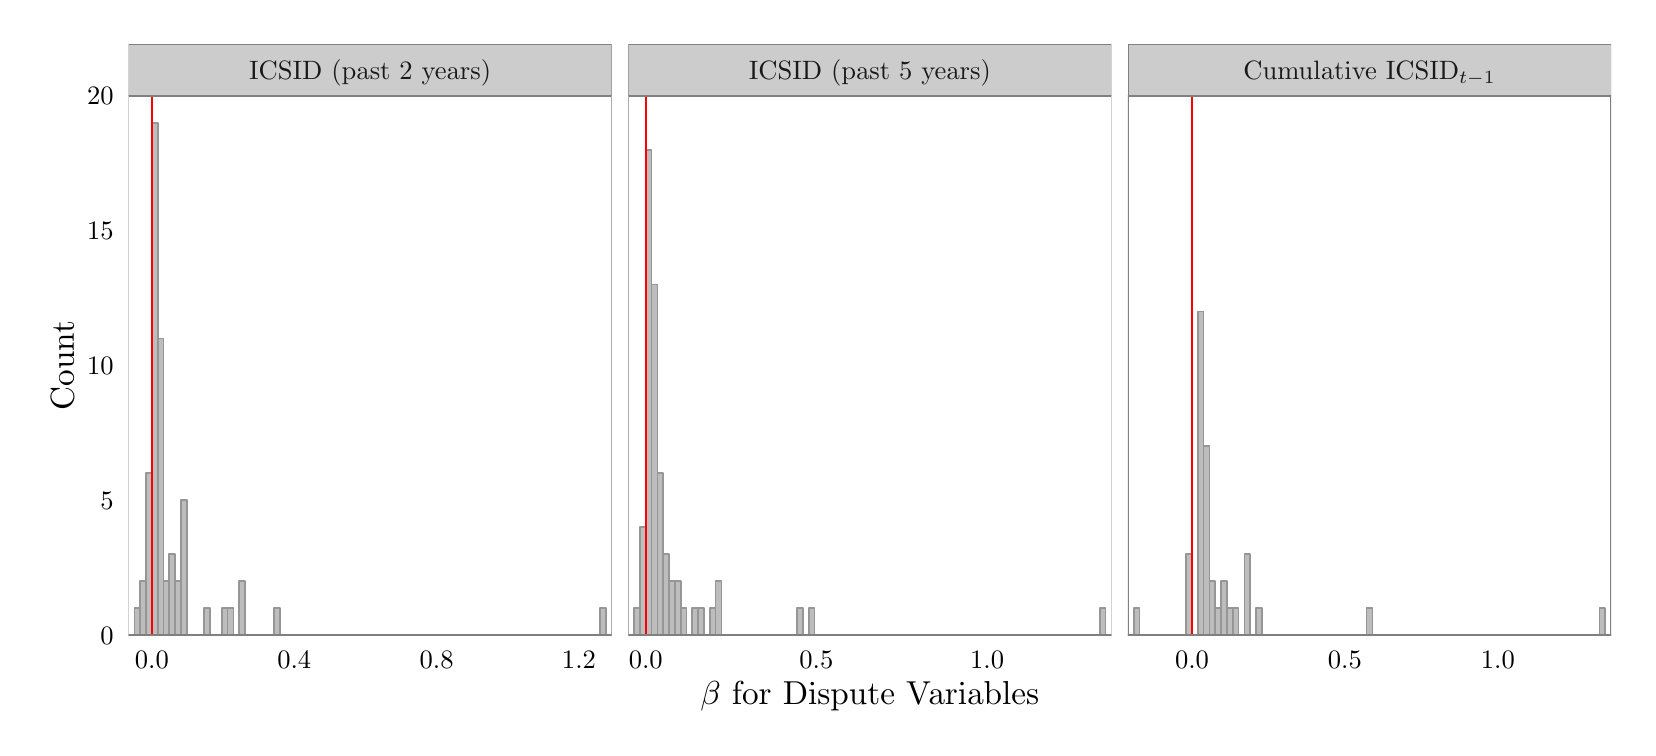
\begin{tikzpicture}[x=1pt,y=1pt]
\definecolor[named]{drawColor}{rgb}{0.00,0.00,0.00}
\definecolor[named]{fillColor}{rgb}{1.00,1.00,1.00}
\fill[color=fillColor,] (0,0) rectangle (578.16,252.94);
\begin{scope}
\path[clip] (  0.00,  0.00) rectangle (578.16,252.94);
\end{scope}
\begin{scope}
\path[clip] (  0.00,  0.00) rectangle (578.16,252.94);
\end{scope}
\begin{scope}
\path[clip] (  0.00,  0.00) rectangle (578.16,252.94);
\end{scope}
\begin{scope}
\path[clip] (  0.00,  0.00) rectangle (578.16,252.94);
\end{scope}
\begin{scope}
\path[clip] (  0.00,  0.00) rectangle (578.16,252.94);
\end{scope}
\begin{scope}
\path[clip] (  0.00,  0.00) rectangle (578.16,252.94);
\end{scope}
\begin{scope}
\path[clip] (  0.00,  0.00) rectangle (578.16,252.94);
\end{scope}
\begin{scope}
\path[clip] (  0.00,  0.00) rectangle (578.16,252.94);
\end{scope}
\begin{scope}
\path[clip] (  0.00,  0.00) rectangle (578.16,252.94);
\end{scope}
\begin{scope}
\path[clip] (  0.00,  0.00) rectangle (578.16,252.94);
\end{scope}
\begin{scope}
\path[clip] (  0.00,  0.00) rectangle (578.16,252.94);
\end{scope}
\begin{scope}
\path[clip] (  0.00,  0.00) rectangle (578.16,252.94);
\end{scope}
\begin{scope}
\path[clip] (  0.00,  0.00) rectangle (578.16,252.94);
\end{scope}
\begin{scope}
\path[clip] (  0.00,  0.00) rectangle (578.16,252.94);
\definecolor[named]{drawColor}{rgb}{1.00,1.00,1.00}
\definecolor[named]{fillColor}{rgb}{1.00,1.00,1.00}

\draw[color=drawColor,line width= 0.6pt,line cap=round,line join=round,fill=fillColor,] (  0.00,  0.00) rectangle (578.16,252.95);
\end{scope}
\begin{scope}
\path[clip] (  0.00,  0.00) rectangle (578.16,252.94);
\end{scope}
\begin{scope}
\path[clip] ( 36.46, 33.48) rectangle (211.03,228.33);
\definecolor[named]{fillColor}{rgb}{1.00,1.00,1.00}

\draw[fill=fillColor,draw opacity=0.00,] ( 36.46, 33.48) rectangle (211.03,228.33);
\definecolor[named]{drawColor}{rgb}{0.59,0.59,0.59}
\definecolor[named]{fillColor}{rgb}{0.74,0.74,0.74}

\draw[color=drawColor,line width= 0.6pt,line join=round,fill=fillColor,] ( 36.46, 33.48) rectangle ( 38.57, 33.48);

\draw[color=drawColor,line width= 0.6pt,line join=round,fill=fillColor,] ( 38.57, 33.48) rectangle ( 40.67, 43.22);

\draw[color=drawColor,line width= 0.6pt,line join=round,fill=fillColor,] ( 40.67, 33.48) rectangle ( 42.77, 52.96);

\draw[color=drawColor,line width= 0.6pt,line join=round,fill=fillColor,] ( 42.77, 33.48) rectangle ( 44.88, 91.93);

\draw[color=drawColor,line width= 0.6pt,line join=round,fill=fillColor,] ( 44.88, 33.48) rectangle ( 46.98,218.59);

\draw[color=drawColor,line width= 0.6pt,line join=round,fill=fillColor,] ( 46.98, 33.48) rectangle ( 49.08,140.65);

\draw[color=drawColor,line width= 0.6pt,line join=round,fill=fillColor,] ( 49.08, 33.48) rectangle ( 51.18, 52.96);

\draw[color=drawColor,line width= 0.6pt,line join=round,fill=fillColor,] ( 51.18, 33.48) rectangle ( 53.29, 62.70);

\draw[color=drawColor,line width= 0.6pt,line join=round,fill=fillColor,] ( 53.29, 33.48) rectangle ( 55.39, 52.96);

\draw[color=drawColor,line width= 0.6pt,line join=round,fill=fillColor,] ( 55.39, 33.48) rectangle ( 57.49, 82.19);

\draw[color=drawColor,line width= 0.6pt,line join=round,fill=fillColor,] ( 57.49, 33.48) rectangle ( 59.60, 33.48);

\draw[color=drawColor,line width= 0.6pt,line join=round,fill=fillColor,] ( 59.60, 33.48) rectangle ( 61.70, 33.48);

\draw[color=drawColor,line width= 0.6pt,line join=round,fill=fillColor,] ( 61.70, 33.48) rectangle ( 63.80, 33.48);

\draw[color=drawColor,line width= 0.6pt,line join=round,fill=fillColor,] ( 63.80, 33.48) rectangle ( 65.91, 43.22);

\draw[color=drawColor,line width= 0.6pt,line join=round,fill=fillColor,] ( 65.91, 33.48) rectangle ( 68.01, 33.48);

\draw[color=drawColor,line width= 0.6pt,line join=round,fill=fillColor,] ( 68.01, 33.48) rectangle ( 70.11, 33.48);

\draw[color=drawColor,line width= 0.6pt,line join=round,fill=fillColor,] ( 70.11, 33.48) rectangle ( 72.22, 43.22);

\draw[color=drawColor,line width= 0.6pt,line join=round,fill=fillColor,] ( 72.22, 33.48) rectangle ( 74.32, 43.22);

\draw[color=drawColor,line width= 0.6pt,line join=round,fill=fillColor,] ( 74.32, 33.48) rectangle ( 76.42, 33.48);

\draw[color=drawColor,line width= 0.6pt,line join=round,fill=fillColor,] ( 76.42, 33.48) rectangle ( 78.53, 52.96);

\draw[color=drawColor,line width= 0.6pt,line join=round,fill=fillColor,] ( 78.53, 33.48) rectangle ( 80.63, 33.48);

\draw[color=drawColor,line width= 0.6pt,line join=round,fill=fillColor,] ( 80.63, 33.48) rectangle ( 82.73, 33.48);

\draw[color=drawColor,line width= 0.6pt,line join=round,fill=fillColor,] ( 82.73, 33.48) rectangle ( 84.84, 33.48);

\draw[color=drawColor,line width= 0.6pt,line join=round,fill=fillColor,] ( 84.84, 33.48) rectangle ( 86.94, 33.48);

\draw[color=drawColor,line width= 0.6pt,line join=round,fill=fillColor,] ( 86.94, 33.48) rectangle ( 89.04, 33.48);

\draw[color=drawColor,line width= 0.6pt,line join=round,fill=fillColor,] ( 89.04, 33.48) rectangle ( 91.15, 43.22);

\draw[color=drawColor,line width= 0.6pt,line join=round,fill=fillColor,] ( 91.15, 33.48) rectangle ( 93.25, 33.48);

\draw[color=drawColor,line width= 0.6pt,line join=round,fill=fillColor,] ( 93.25, 33.48) rectangle ( 95.35, 33.48);

\draw[color=drawColor,line width= 0.6pt,line join=round,fill=fillColor,] ( 95.35, 33.48) rectangle ( 97.46, 33.48);

\draw[color=drawColor,line width= 0.6pt,line join=round,fill=fillColor,] ( 97.46, 33.48) rectangle ( 99.56, 33.48);

\draw[color=drawColor,line width= 0.6pt,line join=round,fill=fillColor,] ( 99.56, 33.48) rectangle (101.66, 33.48);

\draw[color=drawColor,line width= 0.6pt,line join=round,fill=fillColor,] (101.66, 33.48) rectangle (103.76, 33.48);

\draw[color=drawColor,line width= 0.6pt,line join=round,fill=fillColor,] (103.76, 33.48) rectangle (105.87, 33.48);

\draw[color=drawColor,line width= 0.6pt,line join=round,fill=fillColor,] (105.87, 33.48) rectangle (107.97, 33.48);

\draw[color=drawColor,line width= 0.6pt,line join=round,fill=fillColor,] (107.97, 33.48) rectangle (110.07, 33.48);

\draw[color=drawColor,line width= 0.6pt,line join=round,fill=fillColor,] (110.07, 33.48) rectangle (112.18, 33.48);

\draw[color=drawColor,line width= 0.6pt,line join=round,fill=fillColor,] (112.18, 33.48) rectangle (114.28, 33.48);

\draw[color=drawColor,line width= 0.6pt,line join=round,fill=fillColor,] (114.28, 33.48) rectangle (116.38, 33.48);

\draw[color=drawColor,line width= 0.6pt,line join=round,fill=fillColor,] (116.38, 33.48) rectangle (118.49, 33.48);

\draw[color=drawColor,line width= 0.6pt,line join=round,fill=fillColor,] (118.49, 33.48) rectangle (120.59, 33.48);

\draw[color=drawColor,line width= 0.6pt,line join=round,fill=fillColor,] (120.59, 33.48) rectangle (122.69, 33.48);

\draw[color=drawColor,line width= 0.6pt,line join=round,fill=fillColor,] (122.69, 33.48) rectangle (124.80, 33.48);

\draw[color=drawColor,line width= 0.6pt,line join=round,fill=fillColor,] (124.80, 33.48) rectangle (126.90, 33.48);

\draw[color=drawColor,line width= 0.6pt,line join=round,fill=fillColor,] (126.90, 33.48) rectangle (129.00, 33.48);

\draw[color=drawColor,line width= 0.6pt,line join=round,fill=fillColor,] (129.00, 33.48) rectangle (131.11, 33.48);

\draw[color=drawColor,line width= 0.6pt,line join=round,fill=fillColor,] (131.11, 33.48) rectangle (133.21, 33.48);

\draw[color=drawColor,line width= 0.6pt,line join=round,fill=fillColor,] (133.21, 33.48) rectangle (135.31, 33.48);

\draw[color=drawColor,line width= 0.6pt,line join=round,fill=fillColor,] (135.31, 33.48) rectangle (137.42, 33.48);

\draw[color=drawColor,line width= 0.6pt,line join=round,fill=fillColor,] (137.42, 33.48) rectangle (139.52, 33.48);

\draw[color=drawColor,line width= 0.6pt,line join=round,fill=fillColor,] (139.52, 33.48) rectangle (141.62, 33.48);

\draw[color=drawColor,line width= 0.6pt,line join=round,fill=fillColor,] (141.62, 33.48) rectangle (143.73, 33.48);

\draw[color=drawColor,line width= 0.6pt,line join=round,fill=fillColor,] (143.73, 33.48) rectangle (145.83, 33.48);

\draw[color=drawColor,line width= 0.6pt,line join=round,fill=fillColor,] (145.83, 33.48) rectangle (147.93, 33.48);

\draw[color=drawColor,line width= 0.6pt,line join=round,fill=fillColor,] (147.93, 33.48) rectangle (150.04, 33.48);

\draw[color=drawColor,line width= 0.6pt,line join=round,fill=fillColor,] (150.04, 33.48) rectangle (152.14, 33.48);

\draw[color=drawColor,line width= 0.6pt,line join=round,fill=fillColor,] (152.14, 33.48) rectangle (154.24, 33.48);

\draw[color=drawColor,line width= 0.6pt,line join=round,fill=fillColor,] (154.24, 33.48) rectangle (156.34, 33.48);

\draw[color=drawColor,line width= 0.6pt,line join=round,fill=fillColor,] (156.34, 33.48) rectangle (158.45, 33.48);

\draw[color=drawColor,line width= 0.6pt,line join=round,fill=fillColor,] (158.45, 33.48) rectangle (160.55, 33.48);

\draw[color=drawColor,line width= 0.6pt,line join=round,fill=fillColor,] (160.55, 33.48) rectangle (162.65, 33.48);

\draw[color=drawColor,line width= 0.6pt,line join=round,fill=fillColor,] (162.65, 33.48) rectangle (164.76, 33.48);

\draw[color=drawColor,line width= 0.6pt,line join=round,fill=fillColor,] (164.76, 33.48) rectangle (166.86, 33.48);

\draw[color=drawColor,line width= 0.6pt,line join=round,fill=fillColor,] (166.86, 33.48) rectangle (168.96, 33.48);

\draw[color=drawColor,line width= 0.6pt,line join=round,fill=fillColor,] (168.96, 33.48) rectangle (171.07, 33.48);

\draw[color=drawColor,line width= 0.6pt,line join=round,fill=fillColor,] (171.07, 33.48) rectangle (173.17, 33.48);

\draw[color=drawColor,line width= 0.6pt,line join=round,fill=fillColor,] (173.17, 33.48) rectangle (175.27, 33.48);

\draw[color=drawColor,line width= 0.6pt,line join=round,fill=fillColor,] (175.27, 33.48) rectangle (177.38, 33.48);

\draw[color=drawColor,line width= 0.6pt,line join=round,fill=fillColor,] (177.38, 33.48) rectangle (179.48, 33.48);

\draw[color=drawColor,line width= 0.6pt,line join=round,fill=fillColor,] (179.48, 33.48) rectangle (181.58, 33.48);

\draw[color=drawColor,line width= 0.6pt,line join=round,fill=fillColor,] (181.58, 33.48) rectangle (183.69, 33.48);

\draw[color=drawColor,line width= 0.6pt,line join=round,fill=fillColor,] (183.69, 33.48) rectangle (185.79, 33.48);

\draw[color=drawColor,line width= 0.6pt,line join=round,fill=fillColor,] (185.79, 33.48) rectangle (187.89, 33.48);

\draw[color=drawColor,line width= 0.6pt,line join=round,fill=fillColor,] (187.89, 33.48) rectangle (190.00, 33.48);

\draw[color=drawColor,line width= 0.6pt,line join=round,fill=fillColor,] (190.00, 33.48) rectangle (192.10, 33.48);

\draw[color=drawColor,line width= 0.6pt,line join=round,fill=fillColor,] (192.10, 33.48) rectangle (194.20, 33.48);

\draw[color=drawColor,line width= 0.6pt,line join=round,fill=fillColor,] (194.20, 33.48) rectangle (196.31, 33.48);

\draw[color=drawColor,line width= 0.6pt,line join=round,fill=fillColor,] (196.31, 33.48) rectangle (198.41, 33.48);

\draw[color=drawColor,line width= 0.6pt,line join=round,fill=fillColor,] (198.41, 33.48) rectangle (200.51, 33.48);

\draw[color=drawColor,line width= 0.6pt,line join=round,fill=fillColor,] (200.51, 33.48) rectangle (202.62, 33.48);

\draw[color=drawColor,line width= 0.6pt,line join=round,fill=fillColor,] (202.62, 33.48) rectangle (204.72, 33.48);

\draw[color=drawColor,line width= 0.6pt,line join=round,fill=fillColor,] (204.72, 33.48) rectangle (206.82, 33.48);

\draw[color=drawColor,line width= 0.6pt,line join=round,fill=fillColor,] (206.82, 33.48) rectangle (208.93, 43.22);

\draw[color=drawColor,line width= 0.6pt,line join=round,fill=fillColor,] (208.93, 33.48) rectangle (211.03, 33.48);
\definecolor[named]{drawColor}{rgb}{1.00,0.00,0.00}
\definecolor[named]{fillColor}{rgb}{1.00,0.00,0.00}

\draw[color=drawColor,line width= 0.6pt,line join=round,fill=fillColor,] ( 44.88, 33.48) -- ( 44.88,228.33);
\definecolor[named]{drawColor}{rgb}{0.50,0.50,0.50}

\draw[color=drawColor,line width= 0.6pt,line cap=round,line join=round,fill opacity=0.00,] ( 36.46, 33.48) rectangle (211.03,228.33);
\end{scope}
\begin{scope}
\path[clip] (  0.00,  0.00) rectangle (578.16,252.94);
\end{scope}
\begin{scope}
\path[clip] (217.03, 33.48) rectangle (391.59,228.33);
\definecolor[named]{fillColor}{rgb}{1.00,1.00,1.00}

\draw[fill=fillColor,draw opacity=0.00,] (217.03, 33.48) rectangle (391.59,228.33);
\definecolor[named]{drawColor}{rgb}{0.59,0.59,0.59}
\definecolor[named]{fillColor}{rgb}{0.74,0.74,0.74}

\draw[color=drawColor,line width= 0.6pt,line join=round,fill=fillColor,] (217.03, 33.48) rectangle (219.13, 33.48);

\draw[color=drawColor,line width= 0.6pt,line join=round,fill=fillColor,] (219.13, 33.48) rectangle (221.23, 43.22);

\draw[color=drawColor,line width= 0.6pt,line join=round,fill=fillColor,] (221.23, 33.48) rectangle (223.34, 72.45);

\draw[color=drawColor,line width= 0.6pt,line join=round,fill=fillColor,] (223.34, 33.48) rectangle (225.44,208.85);

\draw[color=drawColor,line width= 0.6pt,line join=round,fill=fillColor,] (225.44, 33.48) rectangle (227.54,160.13);

\draw[color=drawColor,line width= 0.6pt,line join=round,fill=fillColor,] (227.54, 33.48) rectangle (229.65, 91.93);

\draw[color=drawColor,line width= 0.6pt,line join=round,fill=fillColor,] (229.65, 33.48) rectangle (231.75, 62.70);

\draw[color=drawColor,line width= 0.6pt,line join=round,fill=fillColor,] (231.75, 33.48) rectangle (233.85, 52.96);

\draw[color=drawColor,line width= 0.6pt,line join=round,fill=fillColor,] (233.85, 33.48) rectangle (235.96, 52.96);

\draw[color=drawColor,line width= 0.6pt,line join=round,fill=fillColor,] (235.96, 33.48) rectangle (238.06, 43.22);

\draw[color=drawColor,line width= 0.6pt,line join=round,fill=fillColor,] (238.06, 33.48) rectangle (240.16, 33.48);

\draw[color=drawColor,line width= 0.6pt,line join=round,fill=fillColor,] (240.16, 33.48) rectangle (242.27, 43.22);

\draw[color=drawColor,line width= 0.6pt,line join=round,fill=fillColor,] (242.27, 33.48) rectangle (244.37, 43.22);

\draw[color=drawColor,line width= 0.6pt,line join=round,fill=fillColor,] (244.37, 33.48) rectangle (246.47, 33.48);

\draw[color=drawColor,line width= 0.6pt,line join=round,fill=fillColor,] (246.47, 33.48) rectangle (248.58, 43.22);

\draw[color=drawColor,line width= 0.6pt,line join=round,fill=fillColor,] (248.58, 33.48) rectangle (250.68, 52.96);

\draw[color=drawColor,line width= 0.6pt,line join=round,fill=fillColor,] (250.68, 33.48) rectangle (252.78, 33.48);

\draw[color=drawColor,line width= 0.6pt,line join=round,fill=fillColor,] (252.78, 33.48) rectangle (254.89, 33.48);

\draw[color=drawColor,line width= 0.6pt,line join=round,fill=fillColor,] (254.89, 33.48) rectangle (256.99, 33.48);

\draw[color=drawColor,line width= 0.6pt,line join=round,fill=fillColor,] (256.99, 33.48) rectangle (259.09, 33.48);

\draw[color=drawColor,line width= 0.6pt,line join=round,fill=fillColor,] (259.09, 33.48) rectangle (261.20, 33.48);

\draw[color=drawColor,line width= 0.6pt,line join=round,fill=fillColor,] (261.20, 33.48) rectangle (263.30, 33.48);

\draw[color=drawColor,line width= 0.6pt,line join=round,fill=fillColor,] (263.30, 33.48) rectangle (265.40, 33.48);

\draw[color=drawColor,line width= 0.6pt,line join=round,fill=fillColor,] (265.40, 33.48) rectangle (267.51, 33.48);

\draw[color=drawColor,line width= 0.6pt,line join=round,fill=fillColor,] (267.51, 33.48) rectangle (269.61, 33.48);

\draw[color=drawColor,line width= 0.6pt,line join=round,fill=fillColor,] (269.61, 33.48) rectangle (271.71, 33.48);

\draw[color=drawColor,line width= 0.6pt,line join=round,fill=fillColor,] (271.71, 33.48) rectangle (273.81, 33.48);

\draw[color=drawColor,line width= 0.6pt,line join=round,fill=fillColor,] (273.81, 33.48) rectangle (275.92, 33.48);

\draw[color=drawColor,line width= 0.6pt,line join=round,fill=fillColor,] (275.92, 33.48) rectangle (278.02, 33.48);

\draw[color=drawColor,line width= 0.6pt,line join=round,fill=fillColor,] (278.02, 33.48) rectangle (280.12, 43.22);

\draw[color=drawColor,line width= 0.6pt,line join=round,fill=fillColor,] (280.12, 33.48) rectangle (282.23, 33.48);

\draw[color=drawColor,line width= 0.6pt,line join=round,fill=fillColor,] (282.23, 33.48) rectangle (284.33, 43.22);

\draw[color=drawColor,line width= 0.6pt,line join=round,fill=fillColor,] (284.33, 33.48) rectangle (286.43, 33.48);

\draw[color=drawColor,line width= 0.6pt,line join=round,fill=fillColor,] (286.43, 33.48) rectangle (288.54, 33.48);

\draw[color=drawColor,line width= 0.6pt,line join=round,fill=fillColor,] (288.54, 33.48) rectangle (290.64, 33.48);

\draw[color=drawColor,line width= 0.6pt,line join=round,fill=fillColor,] (290.64, 33.48) rectangle (292.74, 33.48);

\draw[color=drawColor,line width= 0.6pt,line join=round,fill=fillColor,] (292.74, 33.48) rectangle (294.85, 33.48);

\draw[color=drawColor,line width= 0.6pt,line join=round,fill=fillColor,] (294.85, 33.48) rectangle (296.95, 33.48);

\draw[color=drawColor,line width= 0.6pt,line join=round,fill=fillColor,] (296.95, 33.48) rectangle (299.05, 33.48);

\draw[color=drawColor,line width= 0.6pt,line join=round,fill=fillColor,] (299.05, 33.48) rectangle (301.16, 33.48);

\draw[color=drawColor,line width= 0.6pt,line join=round,fill=fillColor,] (301.16, 33.48) rectangle (303.26, 33.48);

\draw[color=drawColor,line width= 0.6pt,line join=round,fill=fillColor,] (303.26, 33.48) rectangle (305.36, 33.48);

\draw[color=drawColor,line width= 0.6pt,line join=round,fill=fillColor,] (305.36, 33.48) rectangle (307.47, 33.48);

\draw[color=drawColor,line width= 0.6pt,line join=round,fill=fillColor,] (307.47, 33.48) rectangle (309.57, 33.48);

\draw[color=drawColor,line width= 0.6pt,line join=round,fill=fillColor,] (309.57, 33.48) rectangle (311.67, 33.48);

\draw[color=drawColor,line width= 0.6pt,line join=round,fill=fillColor,] (311.67, 33.48) rectangle (313.78, 33.48);

\draw[color=drawColor,line width= 0.6pt,line join=round,fill=fillColor,] (313.78, 33.48) rectangle (315.88, 33.48);

\draw[color=drawColor,line width= 0.6pt,line join=round,fill=fillColor,] (315.88, 33.48) rectangle (317.98, 33.48);

\draw[color=drawColor,line width= 0.6pt,line join=round,fill=fillColor,] (317.98, 33.48) rectangle (320.09, 33.48);

\draw[color=drawColor,line width= 0.6pt,line join=round,fill=fillColor,] (320.09, 33.48) rectangle (322.19, 33.48);

\draw[color=drawColor,line width= 0.6pt,line join=round,fill=fillColor,] (322.19, 33.48) rectangle (324.29, 33.48);

\draw[color=drawColor,line width= 0.6pt,line join=round,fill=fillColor,] (324.29, 33.48) rectangle (326.39, 33.48);

\draw[color=drawColor,line width= 0.6pt,line join=round,fill=fillColor,] (326.39, 33.48) rectangle (328.50, 33.48);

\draw[color=drawColor,line width= 0.6pt,line join=round,fill=fillColor,] (328.50, 33.48) rectangle (330.60, 33.48);

\draw[color=drawColor,line width= 0.6pt,line join=round,fill=fillColor,] (330.60, 33.48) rectangle (332.70, 33.48);

\draw[color=drawColor,line width= 0.6pt,line join=round,fill=fillColor,] (332.70, 33.48) rectangle (334.81, 33.48);

\draw[color=drawColor,line width= 0.6pt,line join=round,fill=fillColor,] (334.81, 33.48) rectangle (336.91, 33.48);

\draw[color=drawColor,line width= 0.6pt,line join=round,fill=fillColor,] (336.91, 33.48) rectangle (339.01, 33.48);

\draw[color=drawColor,line width= 0.6pt,line join=round,fill=fillColor,] (339.01, 33.48) rectangle (341.12, 33.48);

\draw[color=drawColor,line width= 0.6pt,line join=round,fill=fillColor,] (341.12, 33.48) rectangle (343.22, 33.48);

\draw[color=drawColor,line width= 0.6pt,line join=round,fill=fillColor,] (343.22, 33.48) rectangle (345.32, 33.48);

\draw[color=drawColor,line width= 0.6pt,line join=round,fill=fillColor,] (345.32, 33.48) rectangle (347.43, 33.48);

\draw[color=drawColor,line width= 0.6pt,line join=round,fill=fillColor,] (347.43, 33.48) rectangle (349.53, 33.48);

\draw[color=drawColor,line width= 0.6pt,line join=round,fill=fillColor,] (349.53, 33.48) rectangle (351.63, 33.48);

\draw[color=drawColor,line width= 0.6pt,line join=round,fill=fillColor,] (351.63, 33.48) rectangle (353.74, 33.48);

\draw[color=drawColor,line width= 0.6pt,line join=round,fill=fillColor,] (353.74, 33.48) rectangle (355.84, 33.48);

\draw[color=drawColor,line width= 0.6pt,line join=round,fill=fillColor,] (355.84, 33.48) rectangle (357.94, 33.48);

\draw[color=drawColor,line width= 0.6pt,line join=round,fill=fillColor,] (357.94, 33.48) rectangle (360.05, 33.48);

\draw[color=drawColor,line width= 0.6pt,line join=round,fill=fillColor,] (360.05, 33.48) rectangle (362.15, 33.48);

\draw[color=drawColor,line width= 0.6pt,line join=round,fill=fillColor,] (362.15, 33.48) rectangle (364.25, 33.48);

\draw[color=drawColor,line width= 0.6pt,line join=round,fill=fillColor,] (364.25, 33.48) rectangle (366.36, 33.48);

\draw[color=drawColor,line width= 0.6pt,line join=round,fill=fillColor,] (366.36, 33.48) rectangle (368.46, 33.48);

\draw[color=drawColor,line width= 0.6pt,line join=round,fill=fillColor,] (368.46, 33.48) rectangle (370.56, 33.48);

\draw[color=drawColor,line width= 0.6pt,line join=round,fill=fillColor,] (370.56, 33.48) rectangle (372.67, 33.48);

\draw[color=drawColor,line width= 0.6pt,line join=round,fill=fillColor,] (372.67, 33.48) rectangle (374.77, 33.48);

\draw[color=drawColor,line width= 0.6pt,line join=round,fill=fillColor,] (374.77, 33.48) rectangle (376.87, 33.48);

\draw[color=drawColor,line width= 0.6pt,line join=round,fill=fillColor,] (376.87, 33.48) rectangle (378.97, 33.48);

\draw[color=drawColor,line width= 0.6pt,line join=round,fill=fillColor,] (378.97, 33.48) rectangle (381.08, 33.48);

\draw[color=drawColor,line width= 0.6pt,line join=round,fill=fillColor,] (381.08, 33.48) rectangle (383.18, 33.48);

\draw[color=drawColor,line width= 0.6pt,line join=round,fill=fillColor,] (383.18, 33.48) rectangle (385.28, 33.48);

\draw[color=drawColor,line width= 0.6pt,line join=round,fill=fillColor,] (385.28, 33.48) rectangle (387.39, 33.48);

\draw[color=drawColor,line width= 0.6pt,line join=round,fill=fillColor,] (387.39, 33.48) rectangle (389.49, 43.22);

\draw[color=drawColor,line width= 0.6pt,line join=round,fill=fillColor,] (389.49, 33.48) rectangle (391.59, 33.48);
\definecolor[named]{drawColor}{rgb}{1.00,0.00,0.00}
\definecolor[named]{fillColor}{rgb}{1.00,0.00,0.00}

\draw[color=drawColor,line width= 0.6pt,line join=round,fill=fillColor,] (223.34, 33.48) -- (223.34,228.33);
\definecolor[named]{drawColor}{rgb}{0.50,0.50,0.50}

\draw[color=drawColor,line width= 0.6pt,line cap=round,line join=round,fill opacity=0.00,] (217.03, 33.48) rectangle (391.59,228.33);
\end{scope}
\begin{scope}
\path[clip] (  0.00,  0.00) rectangle (578.16,252.94);
\end{scope}
\begin{scope}
\path[clip] (397.59, 33.48) rectangle (572.16,228.33);
\definecolor[named]{fillColor}{rgb}{1.00,1.00,1.00}

\draw[fill=fillColor,draw opacity=0.00,] (397.59, 33.48) rectangle (572.16,228.33);
\definecolor[named]{drawColor}{rgb}{0.59,0.59,0.59}
\definecolor[named]{fillColor}{rgb}{0.74,0.74,0.74}

\draw[color=drawColor,line width= 0.6pt,line join=round,fill=fillColor,] (397.59, 33.48) rectangle (399.70, 33.48);

\draw[color=drawColor,line width= 0.6pt,line join=round,fill=fillColor,] (399.70, 33.48) rectangle (401.80, 43.22);

\draw[color=drawColor,line width= 0.6pt,line join=round,fill=fillColor,] (401.80, 33.48) rectangle (403.90, 33.48);

\draw[color=drawColor,line width= 0.6pt,line join=round,fill=fillColor,] (403.90, 33.48) rectangle (406.01, 33.48);

\draw[color=drawColor,line width= 0.6pt,line join=round,fill=fillColor,] (406.01, 33.48) rectangle (408.11, 33.48);

\draw[color=drawColor,line width= 0.6pt,line join=round,fill=fillColor,] (408.11, 33.48) rectangle (410.21, 33.48);

\draw[color=drawColor,line width= 0.6pt,line join=round,fill=fillColor,] (410.21, 33.48) rectangle (412.32, 33.48);

\draw[color=drawColor,line width= 0.6pt,line join=round,fill=fillColor,] (412.32, 33.48) rectangle (414.42, 33.48);

\draw[color=drawColor,line width= 0.6pt,line join=round,fill=fillColor,] (414.42, 33.48) rectangle (416.52, 33.48);

\draw[color=drawColor,line width= 0.6pt,line join=round,fill=fillColor,] (416.52, 33.48) rectangle (418.63, 33.48);

\draw[color=drawColor,line width= 0.6pt,line join=round,fill=fillColor,] (418.63, 33.48) rectangle (420.73, 62.70);

\draw[color=drawColor,line width= 0.6pt,line join=round,fill=fillColor,] (422.83, 33.48) rectangle (424.94,150.39);

\draw[color=drawColor,line width= 0.6pt,line join=round,fill=fillColor,] (424.94, 33.48) rectangle (427.04,101.68);

\draw[color=drawColor,line width= 0.6pt,line join=round,fill=fillColor,] (427.04, 33.48) rectangle (429.14, 52.96);

\draw[color=drawColor,line width= 0.6pt,line join=round,fill=fillColor,] (429.14, 33.48) rectangle (431.25, 43.22);

\draw[color=drawColor,line width= 0.6pt,line join=round,fill=fillColor,] (431.25, 33.48) rectangle (433.35, 52.96);

\draw[color=drawColor,line width= 0.6pt,line join=round,fill=fillColor,] (433.35, 33.48) rectangle (435.45, 43.22);

\draw[color=drawColor,line width= 0.6pt,line join=round,fill=fillColor,] (435.45, 33.48) rectangle (437.55, 43.22);

\draw[color=drawColor,line width= 0.6pt,line join=round,fill=fillColor,] (437.55, 33.48) rectangle (439.66, 33.48);

\draw[color=drawColor,line width= 0.6pt,line join=round,fill=fillColor,] (439.66, 33.48) rectangle (441.76, 62.70);

\draw[color=drawColor,line width= 0.6pt,line join=round,fill=fillColor,] (441.76, 33.48) rectangle (443.86, 33.48);

\draw[color=drawColor,line width= 0.6pt,line join=round,fill=fillColor,] (443.86, 33.48) rectangle (445.97, 43.22);

\draw[color=drawColor,line width= 0.6pt,line join=round,fill=fillColor,] (445.97, 33.48) rectangle (448.07, 33.48);

\draw[color=drawColor,line width= 0.6pt,line join=round,fill=fillColor,] (448.07, 33.48) rectangle (450.17, 33.48);

\draw[color=drawColor,line width= 0.6pt,line join=round,fill=fillColor,] (450.17, 33.48) rectangle (452.28, 33.48);

\draw[color=drawColor,line width= 0.6pt,line join=round,fill=fillColor,] (452.28, 33.48) rectangle (454.38, 33.48);

\draw[color=drawColor,line width= 0.6pt,line join=round,fill=fillColor,] (454.38, 33.48) rectangle (456.48, 33.48);

\draw[color=drawColor,line width= 0.6pt,line join=round,fill=fillColor,] (456.48, 33.48) rectangle (458.59, 33.48);

\draw[color=drawColor,line width= 0.6pt,line join=round,fill=fillColor,] (458.59, 33.48) rectangle (460.69, 33.48);

\draw[color=drawColor,line width= 0.6pt,line join=round,fill=fillColor,] (460.69, 33.48) rectangle (462.79, 33.48);

\draw[color=drawColor,line width= 0.6pt,line join=round,fill=fillColor,] (462.79, 33.48) rectangle (464.90, 33.48);

\draw[color=drawColor,line width= 0.6pt,line join=round,fill=fillColor,] (464.90, 33.48) rectangle (467.00, 33.48);

\draw[color=drawColor,line width= 0.6pt,line join=round,fill=fillColor,] (467.00, 33.48) rectangle (469.10, 33.48);

\draw[color=drawColor,line width= 0.6pt,line join=round,fill=fillColor,] (469.10, 33.48) rectangle (471.21, 33.48);

\draw[color=drawColor,line width= 0.6pt,line join=round,fill=fillColor,] (471.21, 33.48) rectangle (473.31, 33.48);

\draw[color=drawColor,line width= 0.6pt,line join=round,fill=fillColor,] (473.31, 33.48) rectangle (475.41, 33.48);

\draw[color=drawColor,line width= 0.6pt,line join=round,fill=fillColor,] (475.41, 33.48) rectangle (477.52, 33.48);

\draw[color=drawColor,line width= 0.6pt,line join=round,fill=fillColor,] (477.52, 33.48) rectangle (479.62, 33.48);

\draw[color=drawColor,line width= 0.6pt,line join=round,fill=fillColor,] (479.62, 33.48) rectangle (481.72, 33.48);

\draw[color=drawColor,line width= 0.6pt,line join=round,fill=fillColor,] (481.72, 33.48) rectangle (483.83, 33.48);

\draw[color=drawColor,line width= 0.6pt,line join=round,fill=fillColor,] (483.83, 33.48) rectangle (485.93, 43.22);

\draw[color=drawColor,line width= 0.6pt,line join=round,fill=fillColor,] (485.93, 33.48) rectangle (488.03, 33.48);

\draw[color=drawColor,line width= 0.6pt,line join=round,fill=fillColor,] (488.03, 33.48) rectangle (490.14, 33.48);

\draw[color=drawColor,line width= 0.6pt,line join=round,fill=fillColor,] (490.14, 33.48) rectangle (492.24, 33.48);

\draw[color=drawColor,line width= 0.6pt,line join=round,fill=fillColor,] (492.24, 33.48) rectangle (494.34, 33.48);

\draw[color=drawColor,line width= 0.6pt,line join=round,fill=fillColor,] (494.34, 33.48) rectangle (496.44, 33.48);

\draw[color=drawColor,line width= 0.6pt,line join=round,fill=fillColor,] (496.44, 33.48) rectangle (498.55, 33.48);

\draw[color=drawColor,line width= 0.6pt,line join=round,fill=fillColor,] (498.55, 33.48) rectangle (500.65, 33.48);

\draw[color=drawColor,line width= 0.6pt,line join=round,fill=fillColor,] (500.65, 33.48) rectangle (502.75, 33.48);

\draw[color=drawColor,line width= 0.6pt,line join=round,fill=fillColor,] (502.75, 33.48) rectangle (504.86, 33.48);

\draw[color=drawColor,line width= 0.6pt,line join=round,fill=fillColor,] (504.86, 33.48) rectangle (506.96, 33.48);

\draw[color=drawColor,line width= 0.6pt,line join=round,fill=fillColor,] (506.96, 33.48) rectangle (509.06, 33.48);

\draw[color=drawColor,line width= 0.6pt,line join=round,fill=fillColor,] (509.06, 33.48) rectangle (511.17, 33.48);

\draw[color=drawColor,line width= 0.6pt,line join=round,fill=fillColor,] (511.17, 33.48) rectangle (513.27, 33.48);

\draw[color=drawColor,line width= 0.6pt,line join=round,fill=fillColor,] (513.27, 33.48) rectangle (515.37, 33.48);

\draw[color=drawColor,line width= 0.6pt,line join=round,fill=fillColor,] (515.37, 33.48) rectangle (517.48, 33.48);

\draw[color=drawColor,line width= 0.6pt,line join=round,fill=fillColor,] (517.48, 33.48) rectangle (519.58, 33.48);

\draw[color=drawColor,line width= 0.6pt,line join=round,fill=fillColor,] (519.58, 33.48) rectangle (521.68, 33.48);

\draw[color=drawColor,line width= 0.6pt,line join=round,fill=fillColor,] (521.68, 33.48) rectangle (523.79, 33.48);

\draw[color=drawColor,line width= 0.6pt,line join=round,fill=fillColor,] (523.79, 33.48) rectangle (525.89, 33.48);

\draw[color=drawColor,line width= 0.6pt,line join=round,fill=fillColor,] (525.89, 33.48) rectangle (527.99, 33.48);

\draw[color=drawColor,line width= 0.6pt,line join=round,fill=fillColor,] (527.99, 33.48) rectangle (530.10, 33.48);

\draw[color=drawColor,line width= 0.6pt,line join=round,fill=fillColor,] (530.10, 33.48) rectangle (532.20, 33.48);

\draw[color=drawColor,line width= 0.6pt,line join=round,fill=fillColor,] (532.20, 33.48) rectangle (534.30, 33.48);

\draw[color=drawColor,line width= 0.6pt,line join=round,fill=fillColor,] (534.30, 33.48) rectangle (536.41, 33.48);

\draw[color=drawColor,line width= 0.6pt,line join=round,fill=fillColor,] (536.41, 33.48) rectangle (538.51, 33.48);

\draw[color=drawColor,line width= 0.6pt,line join=round,fill=fillColor,] (538.51, 33.48) rectangle (540.61, 33.48);

\draw[color=drawColor,line width= 0.6pt,line join=round,fill=fillColor,] (540.61, 33.48) rectangle (542.72, 33.48);

\draw[color=drawColor,line width= 0.6pt,line join=round,fill=fillColor,] (542.72, 33.48) rectangle (544.82, 33.48);

\draw[color=drawColor,line width= 0.6pt,line join=round,fill=fillColor,] (544.82, 33.48) rectangle (546.92, 33.48);

\draw[color=drawColor,line width= 0.6pt,line join=round,fill=fillColor,] (546.92, 33.48) rectangle (549.02, 33.48);

\draw[color=drawColor,line width= 0.6pt,line join=round,fill=fillColor,] (549.02, 33.48) rectangle (551.13, 33.48);

\draw[color=drawColor,line width= 0.6pt,line join=round,fill=fillColor,] (551.13, 33.48) rectangle (553.23, 33.48);

\draw[color=drawColor,line width= 0.6pt,line join=round,fill=fillColor,] (553.23, 33.48) rectangle (555.33, 33.48);

\draw[color=drawColor,line width= 0.6pt,line join=round,fill=fillColor,] (555.33, 33.48) rectangle (557.44, 33.48);

\draw[color=drawColor,line width= 0.6pt,line join=round,fill=fillColor,] (557.44, 33.48) rectangle (559.54, 33.48);

\draw[color=drawColor,line width= 0.6pt,line join=round,fill=fillColor,] (559.54, 33.48) rectangle (561.64, 33.48);

\draw[color=drawColor,line width= 0.6pt,line join=round,fill=fillColor,] (561.64, 33.48) rectangle (563.75, 33.48);

\draw[color=drawColor,line width= 0.6pt,line join=round,fill=fillColor,] (563.75, 33.48) rectangle (565.85, 33.48);

\draw[color=drawColor,line width= 0.6pt,line join=round,fill=fillColor,] (565.85, 33.48) rectangle (567.95, 33.48);

\draw[color=drawColor,line width= 0.6pt,line join=round,fill=fillColor,] (567.95, 33.48) rectangle (570.06, 43.22);

\draw[color=drawColor,line width= 0.6pt,line join=round,fill=fillColor,] (570.06, 33.48) rectangle (572.16, 33.48);
\definecolor[named]{drawColor}{rgb}{1.00,0.00,0.00}
\definecolor[named]{fillColor}{rgb}{1.00,0.00,0.00}

\draw[color=drawColor,line width= 0.6pt,line join=round,fill=fillColor,] (420.73, 33.48) -- (420.73,228.33);
\definecolor[named]{drawColor}{rgb}{0.50,0.50,0.50}

\draw[color=drawColor,line width= 0.6pt,line cap=round,line join=round,fill opacity=0.00,] (397.59, 33.48) rectangle (572.16,228.33);
\end{scope}
\begin{scope}
\path[clip] (  0.00,  0.00) rectangle (578.16,252.94);
\end{scope}
\begin{scope}
\path[clip] (  0.00,  0.00) rectangle (578.16,252.94);
\end{scope}
\begin{scope}
\path[clip] (  0.00,  0.00) rectangle (578.16,252.94);
\end{scope}
\begin{scope}
\path[clip] ( 36.46,228.33) rectangle (211.03,246.95);
\definecolor[named]{drawColor}{rgb}{0.50,0.50,0.50}
\definecolor[named]{fillColor}{rgb}{0.80,0.80,0.80}

\draw[color=drawColor,line width= 0.2pt,line cap=round,line join=round,fill=fillColor,] ( 36.46,228.33) rectangle (211.03,246.95);
\definecolor[named]{drawColor}{rgb}{0.10,0.10,0.10}

\node[color=drawColor,anchor=base,inner sep=0pt, outer sep=0pt, scale=  0.96] at (123.75,234.33) {ICSID  (past 2 years)%
};
\end{scope}
\begin{scope}
\path[clip] ( 36.46,228.33) rectangle (211.03,246.95);
\end{scope}
\begin{scope}
\path[clip] (  0.00,  0.00) rectangle (578.16,252.94);
\end{scope}
\begin{scope}
\path[clip] (  0.00,  0.00) rectangle (578.16,252.94);
\end{scope}
\begin{scope}
\path[clip] (  0.00,  0.00) rectangle (578.16,252.94);
\end{scope}
\begin{scope}
\path[clip] (  0.00,  0.00) rectangle (578.16,252.94);
\end{scope}
\begin{scope}
\path[clip] (  0.00,  0.00) rectangle (578.16,252.94);
\end{scope}
\begin{scope}
\path[clip] (  0.00,  0.00) rectangle (578.16,252.94);
\end{scope}
\begin{scope}
\path[clip] (217.03,228.33) rectangle (391.59,246.95);
\definecolor[named]{drawColor}{rgb}{0.50,0.50,0.50}
\definecolor[named]{fillColor}{rgb}{0.80,0.80,0.80}

\draw[color=drawColor,line width= 0.2pt,line cap=round,line join=round,fill=fillColor,] (217.03,228.33) rectangle (391.59,246.95);
\definecolor[named]{drawColor}{rgb}{0.10,0.10,0.10}

\node[color=drawColor,anchor=base,inner sep=0pt, outer sep=0pt, scale=  0.96] at (304.31,234.33) {ICSID  (past 5 years)%
};
\end{scope}
\begin{scope}
\path[clip] (217.03,228.33) rectangle (391.59,246.95);
\end{scope}
\begin{scope}
\path[clip] (  0.00,  0.00) rectangle (578.16,252.94);
\end{scope}
\begin{scope}
\path[clip] (  0.00,  0.00) rectangle (578.16,252.94);
\end{scope}
\begin{scope}
\path[clip] (  0.00,  0.00) rectangle (578.16,252.94);
\end{scope}
\begin{scope}
\path[clip] (  0.00,  0.00) rectangle (578.16,252.94);
\end{scope}
\begin{scope}
\path[clip] (  0.00,  0.00) rectangle (578.16,252.94);
\end{scope}
\begin{scope}
\path[clip] (  0.00,  0.00) rectangle (578.16,252.94);
\end{scope}
\begin{scope}
\path[clip] (397.59,228.33) rectangle (572.16,246.95);
\definecolor[named]{drawColor}{rgb}{0.50,0.50,0.50}
\definecolor[named]{fillColor}{rgb}{0.80,0.80,0.80}

\draw[color=drawColor,line width= 0.2pt,line cap=round,line join=round,fill=fillColor,] (397.59,228.33) rectangle (572.16,246.95);
\definecolor[named]{drawColor}{rgb}{0.10,0.10,0.10}

\node[color=drawColor,anchor=base,inner sep=0pt, outer sep=0pt, scale=  0.96] at (484.88,234.33) {Cumulative ICSID$_{t-1}$%
};
\end{scope}
\begin{scope}
\path[clip] (397.59,228.33) rectangle (572.16,246.95);
\end{scope}
\begin{scope}
\path[clip] (  0.00,  0.00) rectangle (578.16,252.94);
\end{scope}
\begin{scope}
\path[clip] (  0.00,  0.00) rectangle (578.16,252.94);
\end{scope}
\begin{scope}
\path[clip] (  0.00,  0.00) rectangle (578.16,252.94);
\end{scope}
\begin{scope}
\path[clip] (  0.00,  0.00) rectangle (578.16,252.94);
\end{scope}
\begin{scope}
\path[clip] (  0.00,  0.00) rectangle (578.16,252.94);
\end{scope}
\begin{scope}
\path[clip] (  0.00,  0.00) rectangle (578.16,252.94);
\end{scope}
\begin{scope}
\path[clip] (  0.00,  0.00) rectangle (578.16,252.94);
\end{scope}
\begin{scope}
\path[clip] (  0.00,  0.00) rectangle (578.16,252.94);
\end{scope}
\begin{scope}
\path[clip] (  0.00,  0.00) rectangle (578.16,252.94);
\definecolor[named]{drawColor}{rgb}{0.00,0.00,0.00}

\node[color=drawColor,anchor=base east,inner sep=0pt, outer sep=0pt, scale=  0.96] at ( 31.06, 30.17) {0%
};

\node[color=drawColor,anchor=base east,inner sep=0pt, outer sep=0pt, scale=  0.96] at ( 31.06, 78.88) {5%
};

\node[color=drawColor,anchor=base east,inner sep=0pt, outer sep=0pt, scale=  0.96] at ( 31.06,127.60) {10%
};

\node[color=drawColor,anchor=base east,inner sep=0pt, outer sep=0pt, scale=  0.96] at ( 31.06,176.31) {15%
};

\node[color=drawColor,anchor=base east,inner sep=0pt, outer sep=0pt, scale=  0.96] at ( 31.06,225.03) {20%
};
\end{scope}
\begin{scope}
\path[clip] (  0.00,  0.00) rectangle (578.16,252.94);
\end{scope}
\begin{scope}
\path[clip] (  0.00,  0.00) rectangle (578.16,252.94);
\end{scope}
\begin{scope}
\path[clip] (  0.00,  0.00) rectangle (578.16,252.94);
\end{scope}
\begin{scope}
\path[clip] (  0.00,  0.00) rectangle (578.16,252.94);
\end{scope}
\begin{scope}
\path[clip] (  0.00,  0.00) rectangle (578.16,252.94);
\end{scope}
\begin{scope}
\path[clip] (  0.00,  0.00) rectangle (578.16,252.94);
\end{scope}
\begin{scope}
\path[clip] (  0.00,  0.00) rectangle (578.16,252.94);
\end{scope}
\begin{scope}
\path[clip] (  0.00,  0.00) rectangle (578.16,252.94);
\end{scope}
\begin{scope}
\path[clip] (  0.00,  0.00) rectangle (578.16,252.94);
\end{scope}
\begin{scope}
\path[clip] (  0.00,  0.00) rectangle (578.16,252.94);
\end{scope}
\begin{scope}
\path[clip] (  0.00,  0.00) rectangle (578.16,252.94);
\end{scope}
\begin{scope}
\path[clip] (  0.00,  0.00) rectangle (578.16,252.94);
\end{scope}
\begin{scope}
\path[clip] (  0.00,  0.00) rectangle (578.16,252.94);
\end{scope}
\begin{scope}
\path[clip] (  0.00,  0.00) rectangle (578.16,252.94);
\end{scope}
\begin{scope}
\path[clip] (  0.00,  0.00) rectangle (578.16,252.94);
\end{scope}
\begin{scope}
\path[clip] (  0.00,  0.00) rectangle (578.16,252.94);
\end{scope}
\begin{scope}
\path[clip] (  0.00,  0.00) rectangle (578.16,252.94);
\end{scope}
\begin{scope}
\path[clip] (  0.00,  0.00) rectangle (578.16,252.94);
\definecolor[named]{drawColor}{rgb}{0.00,0.00,0.00}

\node[color=drawColor,anchor=base,inner sep=0pt, outer sep=0pt, scale=  0.96] at ( 44.88, 21.46) {0.0%
};

\node[color=drawColor,anchor=base,inner sep=0pt, outer sep=0pt, scale=  0.96] at ( 96.32, 21.46) {0.4%
};

\node[color=drawColor,anchor=base,inner sep=0pt, outer sep=0pt, scale=  0.96] at (147.76, 21.46) {0.8%
};

\node[color=drawColor,anchor=base,inner sep=0pt, outer sep=0pt, scale=  0.96] at (199.21, 21.46) {1.2%
};
\end{scope}
\begin{scope}
\path[clip] (  0.00,  0.00) rectangle (578.16,252.94);
\end{scope}
\begin{scope}
\path[clip] (  0.00,  0.00) rectangle (578.16,252.94);
\end{scope}
\begin{scope}
\path[clip] (  0.00,  0.00) rectangle (578.16,252.94);
\end{scope}
\begin{scope}
\path[clip] (  0.00,  0.00) rectangle (578.16,252.94);
\end{scope}
\begin{scope}
\path[clip] (  0.00,  0.00) rectangle (578.16,252.94);
\end{scope}
\begin{scope}
\path[clip] (  0.00,  0.00) rectangle (578.16,252.94);
\end{scope}
\begin{scope}
\path[clip] (  0.00,  0.00) rectangle (578.16,252.94);
\end{scope}
\begin{scope}
\path[clip] (  0.00,  0.00) rectangle (578.16,252.94);
\end{scope}
\begin{scope}
\path[clip] (  0.00,  0.00) rectangle (578.16,252.94);
\end{scope}
\begin{scope}
\path[clip] (  0.00,  0.00) rectangle (578.16,252.94);
\end{scope}
\begin{scope}
\path[clip] (  0.00,  0.00) rectangle (578.16,252.94);
\end{scope}
\begin{scope}
\path[clip] (  0.00,  0.00) rectangle (578.16,252.94);
\definecolor[named]{drawColor}{rgb}{0.00,0.00,0.00}

\node[color=drawColor,anchor=base,inner sep=0pt, outer sep=0pt, scale=  0.96] at (223.34, 21.46) {0.0%
};

\node[color=drawColor,anchor=base,inner sep=0pt, outer sep=0pt, scale=  0.96] at (285.02, 21.46) {0.5%
};

\node[color=drawColor,anchor=base,inner sep=0pt, outer sep=0pt, scale=  0.96] at (346.69, 21.46) {1.0%
};
\end{scope}
\begin{scope}
\path[clip] (  0.00,  0.00) rectangle (578.16,252.94);
\end{scope}
\begin{scope}
\path[clip] (  0.00,  0.00) rectangle (578.16,252.94);
\end{scope}
\begin{scope}
\path[clip] (  0.00,  0.00) rectangle (578.16,252.94);
\end{scope}
\begin{scope}
\path[clip] (  0.00,  0.00) rectangle (578.16,252.94);
\end{scope}
\begin{scope}
\path[clip] (  0.00,  0.00) rectangle (578.16,252.94);
\end{scope}
\begin{scope}
\path[clip] (  0.00,  0.00) rectangle (578.16,252.94);
\end{scope}
\begin{scope}
\path[clip] (  0.00,  0.00) rectangle (578.16,252.94);
\end{scope}
\begin{scope}
\path[clip] (  0.00,  0.00) rectangle (578.16,252.94);
\end{scope}
\begin{scope}
\path[clip] (  0.00,  0.00) rectangle (578.16,252.94);
\end{scope}
\begin{scope}
\path[clip] (  0.00,  0.00) rectangle (578.16,252.94);
\end{scope}
\begin{scope}
\path[clip] (  0.00,  0.00) rectangle (578.16,252.94);
\end{scope}
\begin{scope}
\path[clip] (  0.00,  0.00) rectangle (578.16,252.94);
\definecolor[named]{drawColor}{rgb}{0.00,0.00,0.00}

\node[color=drawColor,anchor=base,inner sep=0pt, outer sep=0pt, scale=  0.96] at (420.73, 21.46) {0.0%
};

\node[color=drawColor,anchor=base,inner sep=0pt, outer sep=0pt, scale=  0.96] at (475.99, 21.46) {0.5%
};

\node[color=drawColor,anchor=base,inner sep=0pt, outer sep=0pt, scale=  0.96] at (531.25, 21.46) {1.0%
};
\end{scope}
\begin{scope}
\path[clip] (  0.00,  0.00) rectangle (578.16,252.94);
\end{scope}
\begin{scope}
\path[clip] (  0.00,  0.00) rectangle (578.16,252.94);
\end{scope}
\begin{scope}
\path[clip] (  0.00,  0.00) rectangle (578.16,252.94);
\end{scope}
\begin{scope}
\path[clip] (  0.00,  0.00) rectangle (578.16,252.94);
\end{scope}
\begin{scope}
\path[clip] (  0.00,  0.00) rectangle (578.16,252.94);
\end{scope}
\begin{scope}
\path[clip] (  0.00,  0.00) rectangle (578.16,252.94);
\definecolor[named]{drawColor}{rgb}{0.00,0.00,0.00}

\node[color=drawColor,anchor=base,inner sep=0pt, outer sep=0pt, scale=  1.20] at (304.31,  8.40) {$\beta$ for Dispute Variables%
};
\end{scope}
\begin{scope}
\path[clip] (  0.00,  0.00) rectangle (578.16,252.94);
\end{scope}
\begin{scope}
\path[clip] (  0.00,  0.00) rectangle (578.16,252.94);
\end{scope}
\begin{scope}
\path[clip] (  0.00,  0.00) rectangle (578.16,252.94);
\definecolor[named]{drawColor}{rgb}{0.00,0.00,0.00}

\node[rotate= 90.00,color=drawColor,anchor=base,inner sep=0pt, outer sep=0pt, scale=  1.20] at ( 16.66,130.90) {Count%
};
\end{scope}
\begin{scope}
\path[clip] (  0.00,  0.00) rectangle (578.16,252.94);
\end{scope}
\begin{scope}
\path[clip] (  0.00,  0.00) rectangle (578.16,252.94);
\end{scope}
\begin{scope}
\path[clip] (  0.00,  0.00) rectangle (578.16,252.94);
\end{scope}
\begin{scope}
\path[clip] (  0.00,  0.00) rectangle (578.16,252.94);
\end{scope}
\begin{scope}
\path[clip] (  0.00,  0.00) rectangle (578.16,252.94);
\end{scope}
\end{tikzpicture}
}	
\end{figure}

\end{frame}
%%%%%%%%%%%%%%%%%%%%%%%%%%%%%%%%%%%%%%%%%

%%%%%%%%%%%%%%%%%%%%%%%%%%%%%%%%%%%%%%%%%
\begin{frame}
\frametitle{Adding in some controls...}

\begin{figure}[ht]
	\centering
	\vspace{-5mm}
	\resizebox{1\textwidth}{!}{% Created by tikzDevice version 0.6.1 on 2016-03-17 13:37:26
% !TEX encoding = UTF-8 Unicode
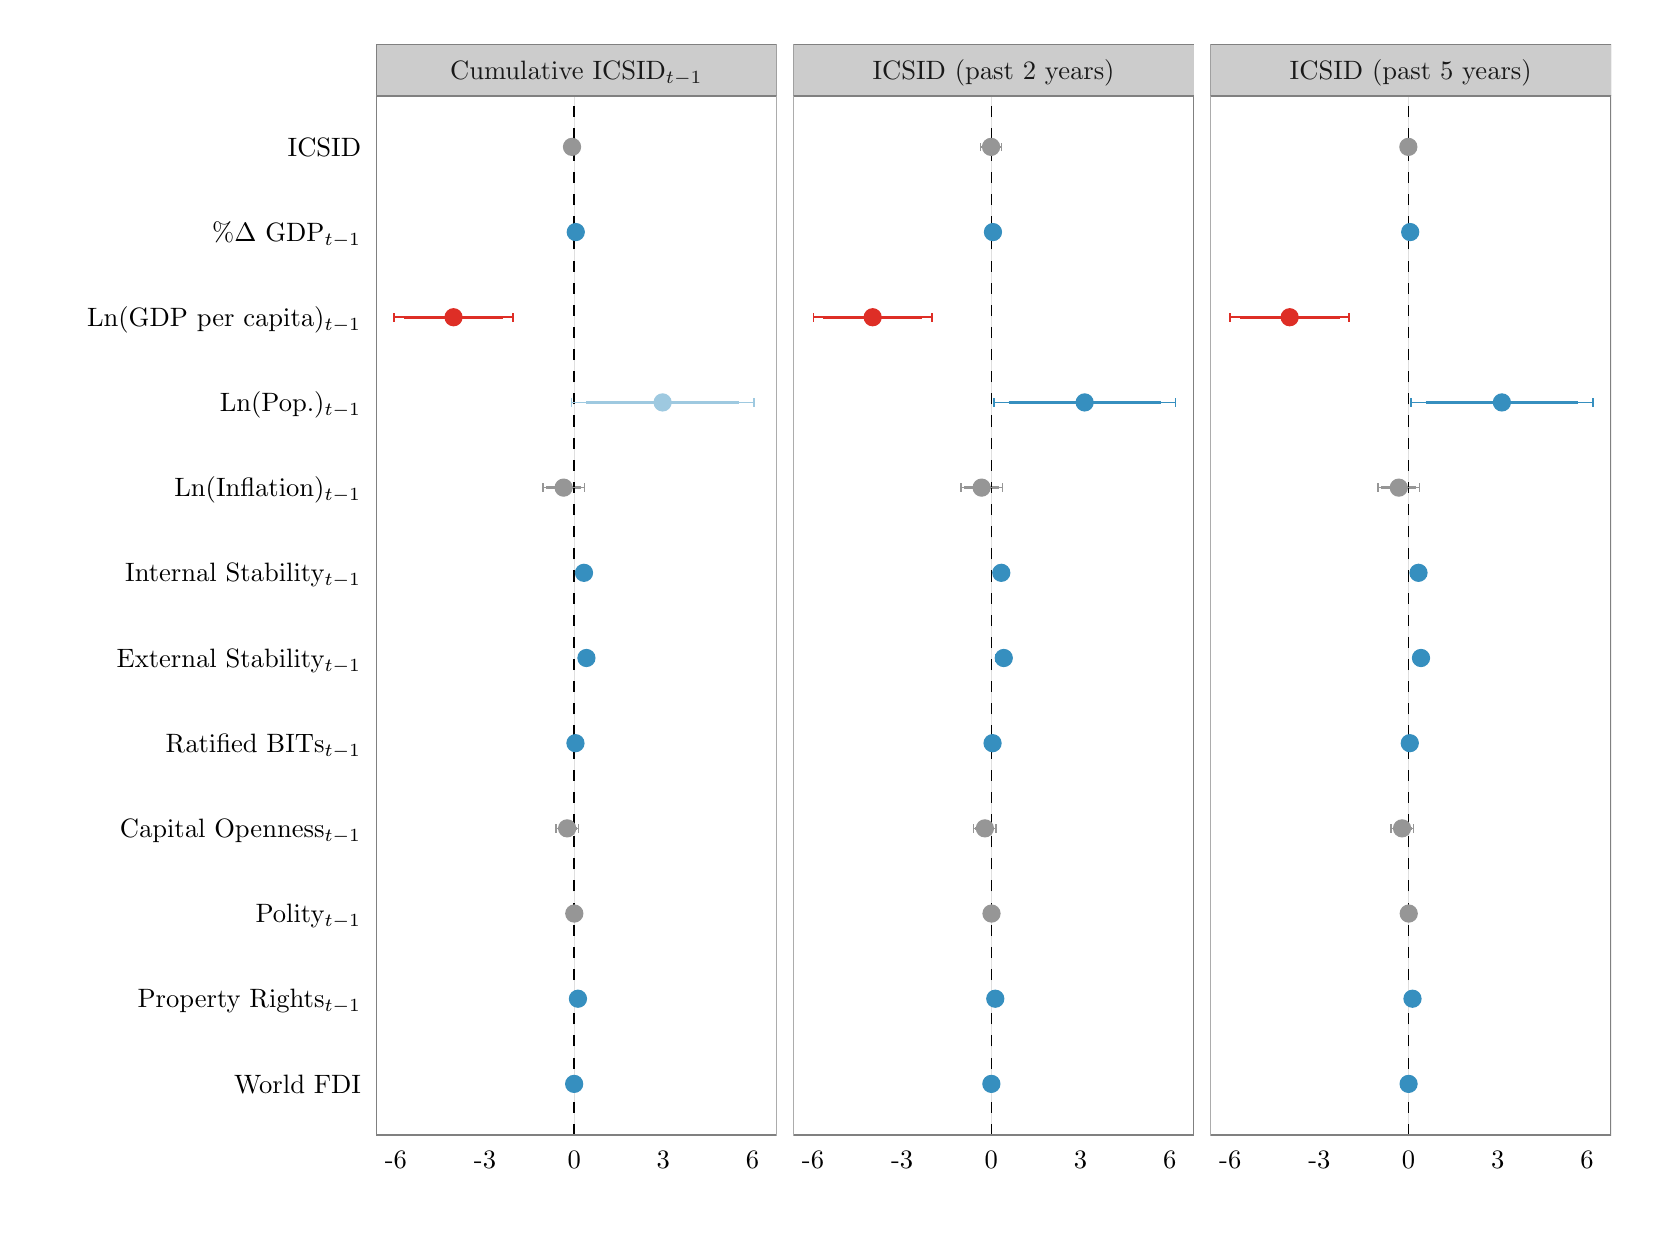
\begin{tikzpicture}[x=1pt,y=1pt]
\definecolor[named]{drawColor}{rgb}{0.00,0.00,0.00}
\definecolor[named]{fillColor}{rgb}{1.00,1.00,1.00}
\fill[color=fillColor,] (0,0) rectangle (578.16,433.62);
\begin{scope}
\path[clip] (  0.00,  0.00) rectangle (578.16,433.62);
\end{scope}
\begin{scope}
\path[clip] (  0.00,  0.00) rectangle (578.16,433.62);
\end{scope}
\begin{scope}
\path[clip] (  0.00,  0.00) rectangle (578.16,433.62);
\end{scope}
\begin{scope}
\path[clip] (  0.00,  0.00) rectangle (578.16,433.62);
\end{scope}
\begin{scope}
\path[clip] (  0.00,  0.00) rectangle (578.16,433.62);
\end{scope}
\begin{scope}
\path[clip] (  0.00,  0.00) rectangle (578.16,433.62);
\end{scope}
\begin{scope}
\path[clip] (  0.00,  0.00) rectangle (578.16,433.62);
\end{scope}
\begin{scope}
\path[clip] (  0.00,  0.00) rectangle (578.16,433.62);
\end{scope}
\begin{scope}
\path[clip] (  0.00,  0.00) rectangle (578.16,433.62);
\end{scope}
\begin{scope}
\path[clip] (  0.00,  0.00) rectangle (578.16,433.62);
\end{scope}
\begin{scope}
\path[clip] (  0.00,  0.00) rectangle (578.16,433.62);
\end{scope}
\begin{scope}
\path[clip] (  0.00,  0.00) rectangle (578.16,433.62);
\end{scope}
\begin{scope}
\path[clip] (  0.00,  0.00) rectangle (578.16,433.62);
\end{scope}
\begin{scope}
\path[clip] (  0.00,  0.00) rectangle (578.16,433.62);
\definecolor[named]{drawColor}{rgb}{1.00,1.00,1.00}
\definecolor[named]{fillColor}{rgb}{1.00,1.00,1.00}

\draw[color=drawColor,line width= 0.6pt,line cap=round,line join=round,fill=fillColor,] (  0.00,  0.00) rectangle (578.16,433.62);
\end{scope}
\begin{scope}
\path[clip] (  0.00,  0.00) rectangle (578.16,433.62);
\end{scope}
\begin{scope}
\path[clip] (125.88, 33.48) rectangle (270.64,409.01);
\definecolor[named]{fillColor}{rgb}{1.00,1.00,1.00}

\draw[fill=fillColor,draw opacity=0.00,] (125.88, 33.48) rectangle (270.64,409.01);
\definecolor[named]{drawColor}{rgb}{0.59,0.59,0.59}
\definecolor[named]{fillColor}{rgb}{0.59,0.59,0.59}

\draw[color=drawColor,line width= 0.3pt,line join=round,fill=fillColor,fill opacity=0.30,draw opacity=0.30,] (195.31,390.54) -- (198.08,390.54);
\definecolor[named]{drawColor}{rgb}{0.21,0.56,0.75}
\definecolor[named]{fillColor}{rgb}{0.21,0.56,0.75}

\draw[color=drawColor,line width= 0.3pt,line join=round,fill=fillColor,fill opacity=0.30,draw opacity=0.30,] (197.48,359.76) -- (198.63,359.76);
\definecolor[named]{drawColor}{rgb}{0.87,0.18,0.15}
\definecolor[named]{fillColor}{rgb}{0.87,0.18,0.15}

\draw[color=drawColor,line width= 0.3pt,line join=round,fill=fillColor,fill opacity=0.30,draw opacity=0.30,] (132.46,328.98) -- (175.30,328.98);
\definecolor[named]{drawColor}{rgb}{0.62,0.79,0.88}
\definecolor[named]{fillColor}{rgb}{0.62,0.79,0.88}

\draw[color=drawColor,line width= 0.3pt,line join=round,fill=fillColor,fill opacity=0.30,draw opacity=0.30,] (196.52,298.20) -- (262.34,298.20);
\definecolor[named]{drawColor}{rgb}{0.59,0.59,0.59}
\definecolor[named]{fillColor}{rgb}{0.59,0.59,0.59}

\draw[color=drawColor,line width= 0.3pt,line join=round,fill=fillColor,fill opacity=0.30,draw opacity=0.30,] (186.15,267.41) -- (201.19,267.41);
\definecolor[named]{drawColor}{rgb}{0.21,0.56,0.75}
\definecolor[named]{fillColor}{rgb}{0.21,0.56,0.75}

\draw[color=drawColor,line width= 0.3pt,line join=round,fill=fillColor,fill opacity=0.30,draw opacity=0.30,] (198.40,236.63) -- (203.63,236.63);

\draw[color=drawColor,line width= 0.3pt,line join=round,fill=fillColor,fill opacity=0.30,draw opacity=0.30,] (199.15,205.85) -- (204.66,205.85);

\draw[color=drawColor,line width= 0.3pt,line join=round,fill=fillColor,fill opacity=0.30,draw opacity=0.30,] (197.51,175.07) -- (198.37,175.07);
\definecolor[named]{drawColor}{rgb}{0.59,0.59,0.59}
\definecolor[named]{fillColor}{rgb}{0.59,0.59,0.59}

\draw[color=drawColor,line width= 0.3pt,line join=round,fill=fillColor,fill opacity=0.30,draw opacity=0.30,] (190.83,144.29) -- (199.05,144.29);

\draw[color=drawColor,line width= 0.3pt,line join=round,fill=fillColor,fill opacity=0.30,draw opacity=0.30,] (197.25,113.51) -- (197.79,113.51);
\definecolor[named]{drawColor}{rgb}{0.21,0.56,0.75}
\definecolor[named]{fillColor}{rgb}{0.21,0.56,0.75}

\draw[color=drawColor,line width= 0.3pt,line join=round,fill=fillColor,fill opacity=0.30,draw opacity=0.30,] (197.58, 82.73) -- (200.10, 82.73);

\draw[color=drawColor,line width= 0.3pt,line join=round,fill=fillColor,fill opacity=0.30,draw opacity=0.30,] (197.47, 51.95) -- (197.47, 51.95);
\definecolor[named]{drawColor}{rgb}{0.59,0.59,0.59}
\definecolor[named]{fillColor}{rgb}{0.59,0.59,0.59}

\draw[color=drawColor,line width= 1.1pt,line join=round,fill=fillColor,] (195.54,390.54) -- (197.86,390.54);
\definecolor[named]{drawColor}{rgb}{0.21,0.56,0.75}
\definecolor[named]{fillColor}{rgb}{0.21,0.56,0.75}

\draw[color=drawColor,line width= 1.1pt,line join=round,fill=fillColor,] (197.57,359.76) -- (198.53,359.76);
\definecolor[named]{drawColor}{rgb}{0.87,0.18,0.15}
\definecolor[named]{fillColor}{rgb}{0.87,0.18,0.15}

\draw[color=drawColor,line width= 1.1pt,line join=round,fill=fillColor,] (135.90,328.98) -- (171.86,328.98);
\definecolor[named]{drawColor}{rgb}{0.62,0.79,0.88}
\definecolor[named]{fillColor}{rgb}{0.62,0.79,0.88}

\draw[color=drawColor,line width= 1.1pt,line join=round,fill=fillColor,] (201.81,298.20) -- (257.05,298.20);
\definecolor[named]{drawColor}{rgb}{0.59,0.59,0.59}
\definecolor[named]{fillColor}{rgb}{0.59,0.59,0.59}

\draw[color=drawColor,line width= 1.1pt,line join=round,fill=fillColor,] (187.36,267.41) -- (199.98,267.41);
\definecolor[named]{drawColor}{rgb}{0.21,0.56,0.75}
\definecolor[named]{fillColor}{rgb}{0.21,0.56,0.75}

\draw[color=drawColor,line width= 1.1pt,line join=round,fill=fillColor,] (198.82,236.63) -- (203.21,236.63);

\draw[color=drawColor,line width= 1.1pt,line join=round,fill=fillColor,] (199.59,205.85) -- (204.22,205.85);

\draw[color=drawColor,line width= 1.1pt,line join=round,fill=fillColor,] (197.58,175.07) -- (198.31,175.07);
\definecolor[named]{drawColor}{rgb}{0.59,0.59,0.59}
\definecolor[named]{fillColor}{rgb}{0.59,0.59,0.59}

\draw[color=drawColor,line width= 1.1pt,line join=round,fill=fillColor,] (191.49,144.29) -- (198.39,144.29);

\draw[color=drawColor,line width= 1.1pt,line join=round,fill=fillColor,] (197.29,113.51) -- (197.74,113.51);
\definecolor[named]{drawColor}{rgb}{0.21,0.56,0.75}
\definecolor[named]{fillColor}{rgb}{0.21,0.56,0.75}

\draw[color=drawColor,line width= 1.1pt,line join=round,fill=fillColor,] (197.78, 82.73) -- (199.90, 82.73);

\draw[color=drawColor,line width= 1.1pt,line join=round,fill=fillColor,] (197.47, 51.95) -- (197.47, 51.95);
\definecolor[named]{drawColor}{rgb}{0.00,0.00,0.00}
\definecolor[named]{fillColor}{rgb}{0.00,0.00,0.00}

\draw[color=drawColor,line width= 0.6pt,dash pattern=on 4pt off 4pt ,line join=round,fill=fillColor,] (197.47, 33.48) -- (197.47,409.01);
\definecolor[named]{drawColor}{rgb}{0.59,0.59,0.59}
\definecolor[named]{fillColor}{rgb}{0.59,0.59,0.59}

\draw[color=drawColor,line width= 0.4pt,line cap=round,line join=round,fill=fillColor,] (196.70,390.54) circle (  3.09);
\definecolor[named]{drawColor}{rgb}{0.21,0.56,0.75}
\definecolor[named]{fillColor}{rgb}{0.21,0.56,0.75}

\draw[color=drawColor,line width= 0.4pt,line cap=round,line join=round,fill=fillColor,] (198.05,359.76) circle (  3.09);
\definecolor[named]{drawColor}{rgb}{0.87,0.18,0.15}
\definecolor[named]{fillColor}{rgb}{0.87,0.18,0.15}

\draw[color=drawColor,line width= 0.4pt,line cap=round,line join=round,fill=fillColor,] (153.88,328.98) circle (  3.09);
\definecolor[named]{drawColor}{rgb}{0.62,0.79,0.88}
\definecolor[named]{fillColor}{rgb}{0.62,0.79,0.88}

\draw[color=drawColor,line width= 0.4pt,line cap=round,line join=round,fill=fillColor,] (229.43,298.20) circle (  3.09);
\definecolor[named]{drawColor}{rgb}{0.59,0.59,0.59}
\definecolor[named]{fillColor}{rgb}{0.59,0.59,0.59}

\draw[color=drawColor,line width= 0.4pt,line cap=round,line join=round,fill=fillColor,] (193.67,267.41) circle (  3.09);
\definecolor[named]{drawColor}{rgb}{0.21,0.56,0.75}
\definecolor[named]{fillColor}{rgb}{0.21,0.56,0.75}

\draw[color=drawColor,line width= 0.4pt,line cap=round,line join=round,fill=fillColor,] (201.02,236.63) circle (  3.09);

\draw[color=drawColor,line width= 0.4pt,line cap=round,line join=round,fill=fillColor,] (201.90,205.85) circle (  3.09);

\draw[color=drawColor,line width= 0.4pt,line cap=round,line join=round,fill=fillColor,] (197.94,175.07) circle (  3.09);
\definecolor[named]{drawColor}{rgb}{0.59,0.59,0.59}
\definecolor[named]{fillColor}{rgb}{0.59,0.59,0.59}

\draw[color=drawColor,line width= 0.4pt,line cap=round,line join=round,fill=fillColor,] (194.94,144.29) circle (  3.09);

\draw[color=drawColor,line width= 0.4pt,line cap=round,line join=round,fill=fillColor,] (197.52,113.51) circle (  3.09);
\definecolor[named]{drawColor}{rgb}{0.21,0.56,0.75}
\definecolor[named]{fillColor}{rgb}{0.21,0.56,0.75}

\draw[color=drawColor,line width= 0.4pt,line cap=round,line join=round,fill=fillColor,] (198.84, 82.73) circle (  3.09);

\draw[color=drawColor,line width= 0.4pt,line cap=round,line join=round,fill=fillColor,] (197.47, 51.95) circle (  3.09);
\definecolor[named]{drawColor}{rgb}{0.59,0.59,0.59}
\definecolor[named]{fillColor}{rgb}{0.59,0.59,0.59}

\draw[color=drawColor,line width= 0.6pt,line join=round,] (198.08,389.00) --
	(198.08,392.08);

\draw[color=drawColor,line width= 0.6pt,line join=round,] (198.08,390.54) --
	(195.31,390.54);

\draw[color=drawColor,line width= 0.6pt,line join=round,] (195.31,389.00) --
	(195.31,392.08);
\definecolor[named]{drawColor}{rgb}{0.21,0.56,0.75}
\definecolor[named]{fillColor}{rgb}{0.21,0.56,0.75}

\draw[color=drawColor,line width= 0.6pt,line join=round,] (198.63,358.22) --
	(198.63,361.30);

\draw[color=drawColor,line width= 0.6pt,line join=round,] (198.63,359.76) --
	(197.48,359.76);

\draw[color=drawColor,line width= 0.6pt,line join=round,] (197.48,358.22) --
	(197.48,361.30);
\definecolor[named]{drawColor}{rgb}{0.87,0.18,0.15}
\definecolor[named]{fillColor}{rgb}{0.87,0.18,0.15}

\draw[color=drawColor,line width= 0.6pt,line join=round,] (175.30,327.44) --
	(175.30,330.52);

\draw[color=drawColor,line width= 0.6pt,line join=round,] (175.30,328.98) --
	(132.46,328.98);

\draw[color=drawColor,line width= 0.6pt,line join=round,] (132.46,327.44) --
	(132.46,330.52);
\definecolor[named]{drawColor}{rgb}{0.62,0.79,0.88}
\definecolor[named]{fillColor}{rgb}{0.62,0.79,0.88}

\draw[color=drawColor,line width= 0.6pt,line join=round,] (262.34,296.66) --
	(262.34,299.73);

\draw[color=drawColor,line width= 0.6pt,line join=round,] (262.34,298.20) --
	(196.52,298.20);

\draw[color=drawColor,line width= 0.6pt,line join=round,] (196.52,296.66) --
	(196.52,299.73);
\definecolor[named]{drawColor}{rgb}{0.59,0.59,0.59}
\definecolor[named]{fillColor}{rgb}{0.59,0.59,0.59}

\draw[color=drawColor,line width= 0.6pt,line join=round,] (201.19,265.88) --
	(201.19,268.95);

\draw[color=drawColor,line width= 0.6pt,line join=round,] (201.19,267.41) --
	(186.15,267.41);

\draw[color=drawColor,line width= 0.6pt,line join=round,] (186.15,265.88) --
	(186.15,268.95);
\definecolor[named]{drawColor}{rgb}{0.21,0.56,0.75}
\definecolor[named]{fillColor}{rgb}{0.21,0.56,0.75}

\draw[color=drawColor,line width= 0.6pt,line join=round,] (203.63,235.09) --
	(203.63,238.17);

\draw[color=drawColor,line width= 0.6pt,line join=round,] (203.63,236.63) --
	(198.40,236.63);

\draw[color=drawColor,line width= 0.6pt,line join=round,] (198.40,235.09) --
	(198.40,238.17);

\draw[color=drawColor,line width= 0.6pt,line join=round,] (204.66,204.31) --
	(204.66,207.39);

\draw[color=drawColor,line width= 0.6pt,line join=round,] (204.66,205.85) --
	(199.15,205.85);

\draw[color=drawColor,line width= 0.6pt,line join=round,] (199.15,204.31) --
	(199.15,207.39);

\draw[color=drawColor,line width= 0.6pt,line join=round,] (198.37,173.53) --
	(198.37,176.61);

\draw[color=drawColor,line width= 0.6pt,line join=round,] (198.37,175.07) --
	(197.51,175.07);

\draw[color=drawColor,line width= 0.6pt,line join=round,] (197.51,173.53) --
	(197.51,176.61);
\definecolor[named]{drawColor}{rgb}{0.59,0.59,0.59}
\definecolor[named]{fillColor}{rgb}{0.59,0.59,0.59}

\draw[color=drawColor,line width= 0.6pt,line join=round,] (199.05,142.75) --
	(199.05,145.83);

\draw[color=drawColor,line width= 0.6pt,line join=round,] (199.05,144.29) --
	(190.83,144.29);

\draw[color=drawColor,line width= 0.6pt,line join=round,] (190.83,142.75) --
	(190.83,145.83);

\draw[color=drawColor,line width= 0.6pt,line join=round,] (197.79,111.97) --
	(197.79,115.05);

\draw[color=drawColor,line width= 0.6pt,line join=round,] (197.79,113.51) --
	(197.25,113.51);

\draw[color=drawColor,line width= 0.6pt,line join=round,] (197.25,111.97) --
	(197.25,115.05);
\definecolor[named]{drawColor}{rgb}{0.21,0.56,0.75}
\definecolor[named]{fillColor}{rgb}{0.21,0.56,0.75}

\draw[color=drawColor,line width= 0.6pt,line join=round,] (200.10, 81.19) --
	(200.10, 84.27);

\draw[color=drawColor,line width= 0.6pt,line join=round,] (200.10, 82.73) --
	(197.58, 82.73);

\draw[color=drawColor,line width= 0.6pt,line join=round,] (197.58, 81.19) --
	(197.58, 84.27);

\draw[color=drawColor,line width= 0.6pt,line join=round,] (197.47, 50.41) --
	(197.47, 53.48);

\draw[color=drawColor,line width= 0.6pt,line join=round,] (197.47, 51.95) --
	(197.47, 51.95);

\draw[color=drawColor,line width= 0.6pt,line join=round,] (197.47, 50.41) --
	(197.47, 53.48);
\definecolor[named]{drawColor}{rgb}{0.50,0.50,0.50}

\draw[color=drawColor,line width= 0.6pt,line cap=round,line join=round,fill opacity=0.00,] (125.88, 33.48) rectangle (270.64,409.01);
\end{scope}
\begin{scope}
\path[clip] (  0.00,  0.00) rectangle (578.16,433.62);
\end{scope}
\begin{scope}
\path[clip] (276.64, 33.48) rectangle (421.40,409.01);
\definecolor[named]{fillColor}{rgb}{1.00,1.00,1.00}

\draw[fill=fillColor,draw opacity=0.00,] (276.64, 33.48) rectangle (421.40,409.01);
\definecolor[named]{drawColor}{rgb}{0.59,0.59,0.59}
\definecolor[named]{fillColor}{rgb}{0.59,0.59,0.59}

\draw[color=drawColor,line width= 0.3pt,line join=round,fill=fillColor,fill opacity=0.30,draw opacity=0.30,] (344.30,390.54) -- (351.94,390.54);
\definecolor[named]{drawColor}{rgb}{0.21,0.56,0.75}
\definecolor[named]{fillColor}{rgb}{0.21,0.56,0.75}

\draw[color=drawColor,line width= 0.3pt,line join=round,fill=fillColor,fill opacity=0.30,draw opacity=0.30,] (348.23,359.76) -- (349.38,359.76);
\definecolor[named]{drawColor}{rgb}{0.87,0.18,0.15}
\definecolor[named]{fillColor}{rgb}{0.87,0.18,0.15}

\draw[color=drawColor,line width= 0.3pt,line join=round,fill=fillColor,fill opacity=0.30,draw opacity=0.30,] (283.90,328.98) -- (326.77,328.98);
\definecolor[named]{drawColor}{rgb}{0.21,0.56,0.75}
\definecolor[named]{fillColor}{rgb}{0.21,0.56,0.75}

\draw[color=drawColor,line width= 0.3pt,line join=round,fill=fillColor,fill opacity=0.30,draw opacity=0.30,] (349.15,298.20) -- (414.72,298.20);
\definecolor[named]{drawColor}{rgb}{0.59,0.59,0.59}
\definecolor[named]{fillColor}{rgb}{0.59,0.59,0.59}

\draw[color=drawColor,line width= 0.3pt,line join=round,fill=fillColor,fill opacity=0.30,draw opacity=0.30,] (337.20,267.41) -- (352.22,267.41);
\definecolor[named]{drawColor}{rgb}{0.21,0.56,0.75}
\definecolor[named]{fillColor}{rgb}{0.21,0.56,0.75}

\draw[color=drawColor,line width= 0.3pt,line join=round,fill=fillColor,fill opacity=0.30,draw opacity=0.30,] (349.20,236.63) -- (354.43,236.63);

\draw[color=drawColor,line width= 0.3pt,line join=round,fill=fillColor,fill opacity=0.30,draw opacity=0.30,] (349.96,205.85) -- (355.46,205.85);

\draw[color=drawColor,line width= 0.3pt,line join=round,fill=fillColor,fill opacity=0.30,draw opacity=0.30,] (348.23,175.07) -- (349.09,175.07);
\definecolor[named]{drawColor}{rgb}{0.59,0.59,0.59}
\definecolor[named]{fillColor}{rgb}{0.59,0.59,0.59}

\draw[color=drawColor,line width= 0.3pt,line join=round,fill=fillColor,fill opacity=0.30,draw opacity=0.30,] (341.79,144.29) -- (349.99,144.29);

\draw[color=drawColor,line width= 0.3pt,line join=round,fill=fillColor,fill opacity=0.30,draw opacity=0.30,] (348.01,113.51) -- (348.55,113.51);
\definecolor[named]{drawColor}{rgb}{0.21,0.56,0.75}
\definecolor[named]{fillColor}{rgb}{0.21,0.56,0.75}

\draw[color=drawColor,line width= 0.3pt,line join=round,fill=fillColor,fill opacity=0.30,draw opacity=0.30,] (348.37, 82.73) -- (350.90, 82.73);

\draw[color=drawColor,line width= 0.3pt,line join=round,fill=fillColor,fill opacity=0.30,draw opacity=0.30,] (348.23, 51.95) -- (348.23, 51.95);
\definecolor[named]{drawColor}{rgb}{0.59,0.59,0.59}
\definecolor[named]{fillColor}{rgb}{0.59,0.59,0.59}

\draw[color=drawColor,line width= 1.1pt,line join=round,fill=fillColor,] (344.91,390.54) -- (351.33,390.54);
\definecolor[named]{drawColor}{rgb}{0.21,0.56,0.75}
\definecolor[named]{fillColor}{rgb}{0.21,0.56,0.75}

\draw[color=drawColor,line width= 1.1pt,line join=round,fill=fillColor,] (348.32,359.76) -- (349.28,359.76);
\definecolor[named]{drawColor}{rgb}{0.87,0.18,0.15}
\definecolor[named]{fillColor}{rgb}{0.87,0.18,0.15}

\draw[color=drawColor,line width= 1.1pt,line join=round,fill=fillColor,] (287.35,328.98) -- (323.33,328.98);
\definecolor[named]{drawColor}{rgb}{0.21,0.56,0.75}
\definecolor[named]{fillColor}{rgb}{0.21,0.56,0.75}

\draw[color=drawColor,line width= 1.1pt,line join=round,fill=fillColor,] (354.42,298.20) -- (409.45,298.20);
\definecolor[named]{drawColor}{rgb}{0.59,0.59,0.59}
\definecolor[named]{fillColor}{rgb}{0.59,0.59,0.59}

\draw[color=drawColor,line width= 1.1pt,line join=round,fill=fillColor,] (338.41,267.41) -- (351.01,267.41);
\definecolor[named]{drawColor}{rgb}{0.21,0.56,0.75}
\definecolor[named]{fillColor}{rgb}{0.21,0.56,0.75}

\draw[color=drawColor,line width= 1.1pt,line join=round,fill=fillColor,] (349.62,236.63) -- (354.01,236.63);

\draw[color=drawColor,line width= 1.1pt,line join=round,fill=fillColor,] (350.40,205.85) -- (355.02,205.85);

\draw[color=drawColor,line width= 1.1pt,line join=round,fill=fillColor,] (348.30,175.07) -- (349.02,175.07);
\definecolor[named]{drawColor}{rgb}{0.59,0.59,0.59}
\definecolor[named]{fillColor}{rgb}{0.59,0.59,0.59}

\draw[color=drawColor,line width= 1.1pt,line join=round,fill=fillColor,] (342.45,144.29) -- (349.33,144.29);

\draw[color=drawColor,line width= 1.1pt,line join=round,fill=fillColor,] (348.05,113.51) -- (348.50,113.51);
\definecolor[named]{drawColor}{rgb}{0.21,0.56,0.75}
\definecolor[named]{fillColor}{rgb}{0.21,0.56,0.75}

\draw[color=drawColor,line width= 1.1pt,line join=round,fill=fillColor,] (348.58, 82.73) -- (350.69, 82.73);

\draw[color=drawColor,line width= 1.1pt,line join=round,fill=fillColor,] (348.23, 51.95) -- (348.23, 51.95);
\definecolor[named]{drawColor}{rgb}{0.00,0.00,0.00}
\definecolor[named]{fillColor}{rgb}{0.00,0.00,0.00}

\draw[color=drawColor,line width= 0.6pt,dash pattern=on 4pt off 4pt ,line join=round,fill=fillColor,] (348.23, 33.48) -- (348.23,409.01);
\definecolor[named]{drawColor}{rgb}{0.59,0.59,0.59}
\definecolor[named]{fillColor}{rgb}{0.59,0.59,0.59}

\draw[color=drawColor,line width= 0.4pt,line cap=round,line join=round,fill=fillColor,] (348.12,390.54) circle (  3.09);
\definecolor[named]{drawColor}{rgb}{0.21,0.56,0.75}
\definecolor[named]{fillColor}{rgb}{0.21,0.56,0.75}

\draw[color=drawColor,line width= 0.4pt,line cap=round,line join=round,fill=fillColor,] (348.80,359.76) circle (  3.09);
\definecolor[named]{drawColor}{rgb}{0.87,0.18,0.15}
\definecolor[named]{fillColor}{rgb}{0.87,0.18,0.15}

\draw[color=drawColor,line width= 0.4pt,line cap=round,line join=round,fill=fillColor,] (305.34,328.98) circle (  3.09);
\definecolor[named]{drawColor}{rgb}{0.21,0.56,0.75}
\definecolor[named]{fillColor}{rgb}{0.21,0.56,0.75}

\draw[color=drawColor,line width= 0.4pt,line cap=round,line join=round,fill=fillColor,] (381.94,298.20) circle (  3.09);
\definecolor[named]{drawColor}{rgb}{0.59,0.59,0.59}
\definecolor[named]{fillColor}{rgb}{0.59,0.59,0.59}

\draw[color=drawColor,line width= 0.4pt,line cap=round,line join=round,fill=fillColor,] (344.71,267.41) circle (  3.09);
\definecolor[named]{drawColor}{rgb}{0.21,0.56,0.75}
\definecolor[named]{fillColor}{rgb}{0.21,0.56,0.75}

\draw[color=drawColor,line width= 0.4pt,line cap=round,line join=round,fill=fillColor,] (351.81,236.63) circle (  3.09);

\draw[color=drawColor,line width= 0.4pt,line cap=round,line join=round,fill=fillColor,] (352.71,205.85) circle (  3.09);

\draw[color=drawColor,line width= 0.4pt,line cap=round,line join=round,fill=fillColor,] (348.66,175.07) circle (  3.09);
\definecolor[named]{drawColor}{rgb}{0.59,0.59,0.59}
\definecolor[named]{fillColor}{rgb}{0.59,0.59,0.59}

\draw[color=drawColor,line width= 0.4pt,line cap=round,line join=round,fill=fillColor,] (345.89,144.29) circle (  3.09);

\draw[color=drawColor,line width= 0.4pt,line cap=round,line join=round,fill=fillColor,] (348.28,113.51) circle (  3.09);
\definecolor[named]{drawColor}{rgb}{0.21,0.56,0.75}
\definecolor[named]{fillColor}{rgb}{0.21,0.56,0.75}

\draw[color=drawColor,line width= 0.4pt,line cap=round,line join=round,fill=fillColor,] (349.64, 82.73) circle (  3.09);

\draw[color=drawColor,line width= 0.4pt,line cap=round,line join=round,fill=fillColor,] (348.23, 51.95) circle (  3.09);
\definecolor[named]{drawColor}{rgb}{0.59,0.59,0.59}
\definecolor[named]{fillColor}{rgb}{0.59,0.59,0.59}

\draw[color=drawColor,line width= 0.6pt,line join=round,] (351.94,389.00) --
	(351.94,392.08);

\draw[color=drawColor,line width= 0.6pt,line join=round,] (351.94,390.54) --
	(344.30,390.54);

\draw[color=drawColor,line width= 0.6pt,line join=round,] (344.30,389.00) --
	(344.30,392.08);
\definecolor[named]{drawColor}{rgb}{0.21,0.56,0.75}
\definecolor[named]{fillColor}{rgb}{0.21,0.56,0.75}

\draw[color=drawColor,line width= 0.6pt,line join=round,] (349.38,358.22) --
	(349.38,361.30);

\draw[color=drawColor,line width= 0.6pt,line join=round,] (349.38,359.76) --
	(348.23,359.76);

\draw[color=drawColor,line width= 0.6pt,line join=round,] (348.23,358.22) --
	(348.23,361.30);
\definecolor[named]{drawColor}{rgb}{0.87,0.18,0.15}
\definecolor[named]{fillColor}{rgb}{0.87,0.18,0.15}

\draw[color=drawColor,line width= 0.6pt,line join=round,] (326.77,327.44) --
	(326.77,330.52);

\draw[color=drawColor,line width= 0.6pt,line join=round,] (326.77,328.98) --
	(283.90,328.98);

\draw[color=drawColor,line width= 0.6pt,line join=round,] (283.90,327.44) --
	(283.90,330.52);
\definecolor[named]{drawColor}{rgb}{0.21,0.56,0.75}
\definecolor[named]{fillColor}{rgb}{0.21,0.56,0.75}

\draw[color=drawColor,line width= 0.6pt,line join=round,] (414.72,296.66) --
	(414.72,299.73);

\draw[color=drawColor,line width= 0.6pt,line join=round,] (414.72,298.20) --
	(349.15,298.20);

\draw[color=drawColor,line width= 0.6pt,line join=round,] (349.15,296.66) --
	(349.15,299.73);
\definecolor[named]{drawColor}{rgb}{0.59,0.59,0.59}
\definecolor[named]{fillColor}{rgb}{0.59,0.59,0.59}

\draw[color=drawColor,line width= 0.6pt,line join=round,] (352.22,265.88) --
	(352.22,268.95);

\draw[color=drawColor,line width= 0.6pt,line join=round,] (352.22,267.41) --
	(337.20,267.41);

\draw[color=drawColor,line width= 0.6pt,line join=round,] (337.20,265.88) --
	(337.20,268.95);
\definecolor[named]{drawColor}{rgb}{0.21,0.56,0.75}
\definecolor[named]{fillColor}{rgb}{0.21,0.56,0.75}

\draw[color=drawColor,line width= 0.6pt,line join=round,] (354.43,235.09) --
	(354.43,238.17);

\draw[color=drawColor,line width= 0.6pt,line join=round,] (354.43,236.63) --
	(349.20,236.63);

\draw[color=drawColor,line width= 0.6pt,line join=round,] (349.20,235.09) --
	(349.20,238.17);

\draw[color=drawColor,line width= 0.6pt,line join=round,] (355.46,204.31) --
	(355.46,207.39);

\draw[color=drawColor,line width= 0.6pt,line join=round,] (355.46,205.85) --
	(349.96,205.85);

\draw[color=drawColor,line width= 0.6pt,line join=round,] (349.96,204.31) --
	(349.96,207.39);

\draw[color=drawColor,line width= 0.6pt,line join=round,] (349.09,173.53) --
	(349.09,176.61);

\draw[color=drawColor,line width= 0.6pt,line join=round,] (349.09,175.07) --
	(348.23,175.07);

\draw[color=drawColor,line width= 0.6pt,line join=round,] (348.23,173.53) --
	(348.23,176.61);
\definecolor[named]{drawColor}{rgb}{0.59,0.59,0.59}
\definecolor[named]{fillColor}{rgb}{0.59,0.59,0.59}

\draw[color=drawColor,line width= 0.6pt,line join=round,] (349.99,142.75) --
	(349.99,145.83);

\draw[color=drawColor,line width= 0.6pt,line join=round,] (349.99,144.29) --
	(341.79,144.29);

\draw[color=drawColor,line width= 0.6pt,line join=round,] (341.79,142.75) --
	(341.79,145.83);

\draw[color=drawColor,line width= 0.6pt,line join=round,] (348.55,111.97) --
	(348.55,115.05);

\draw[color=drawColor,line width= 0.6pt,line join=round,] (348.55,113.51) --
	(348.01,113.51);

\draw[color=drawColor,line width= 0.6pt,line join=round,] (348.01,111.97) --
	(348.01,115.05);
\definecolor[named]{drawColor}{rgb}{0.21,0.56,0.75}
\definecolor[named]{fillColor}{rgb}{0.21,0.56,0.75}

\draw[color=drawColor,line width= 0.6pt,line join=round,] (350.90, 81.19) --
	(350.90, 84.27);

\draw[color=drawColor,line width= 0.6pt,line join=round,] (350.90, 82.73) --
	(348.37, 82.73);

\draw[color=drawColor,line width= 0.6pt,line join=round,] (348.37, 81.19) --
	(348.37, 84.27);

\draw[color=drawColor,line width= 0.6pt,line join=round,] (348.23, 50.41) --
	(348.23, 53.48);

\draw[color=drawColor,line width= 0.6pt,line join=round,] (348.23, 51.95) --
	(348.23, 51.95);

\draw[color=drawColor,line width= 0.6pt,line join=round,] (348.23, 50.41) --
	(348.23, 53.48);
\definecolor[named]{drawColor}{rgb}{0.50,0.50,0.50}

\draw[color=drawColor,line width= 0.6pt,line cap=round,line join=round,fill opacity=0.00,] (276.64, 33.48) rectangle (421.40,409.01);
\end{scope}
\begin{scope}
\path[clip] (  0.00,  0.00) rectangle (578.16,433.62);
\end{scope}
\begin{scope}
\path[clip] (427.40, 33.48) rectangle (572.16,409.01);
\definecolor[named]{fillColor}{rgb}{1.00,1.00,1.00}

\draw[fill=fillColor,draw opacity=0.00,] (427.40, 33.48) rectangle (572.16,409.01);
\definecolor[named]{drawColor}{rgb}{0.59,0.59,0.59}
\definecolor[named]{fillColor}{rgb}{0.59,0.59,0.59}

\draw[color=drawColor,line width= 0.3pt,line join=round,fill=fillColor,fill opacity=0.30,draw opacity=0.30,] (496.65,390.54) -- (501.14,390.54);
\definecolor[named]{drawColor}{rgb}{0.21,0.56,0.75}
\definecolor[named]{fillColor}{rgb}{0.21,0.56,0.75}

\draw[color=drawColor,line width= 0.3pt,line join=round,fill=fillColor,fill opacity=0.30,draw opacity=0.30,] (498.99,359.76) -- (500.14,359.76);
\definecolor[named]{drawColor}{rgb}{0.87,0.18,0.15}
\definecolor[named]{fillColor}{rgb}{0.87,0.18,0.15}

\draw[color=drawColor,line width= 0.3pt,line join=round,fill=fillColor,fill opacity=0.30,draw opacity=0.30,] (434.54,328.98) -- (477.49,328.98);
\definecolor[named]{drawColor}{rgb}{0.21,0.56,0.75}
\definecolor[named]{fillColor}{rgb}{0.21,0.56,0.75}

\draw[color=drawColor,line width= 0.3pt,line join=round,fill=fillColor,fill opacity=0.30,draw opacity=0.30,] (499.83,298.20) -- (565.58,298.20);
\definecolor[named]{drawColor}{rgb}{0.59,0.59,0.59}
\definecolor[named]{fillColor}{rgb}{0.59,0.59,0.59}

\draw[color=drawColor,line width= 0.3pt,line join=round,fill=fillColor,fill opacity=0.30,draw opacity=0.30,] (487.94,267.41) -- (502.97,267.41);
\definecolor[named]{drawColor}{rgb}{0.21,0.56,0.75}
\definecolor[named]{fillColor}{rgb}{0.21,0.56,0.75}

\draw[color=drawColor,line width= 0.3pt,line join=round,fill=fillColor,fill opacity=0.30,draw opacity=0.30,] (499.96,236.63) -- (505.19,236.63);

\draw[color=drawColor,line width= 0.3pt,line join=round,fill=fillColor,fill opacity=0.30,draw opacity=0.30,] (500.72,205.85) -- (506.23,205.85);

\draw[color=drawColor,line width= 0.3pt,line join=round,fill=fillColor,fill opacity=0.30,draw opacity=0.30,] (498.99,175.07) -- (499.85,175.07);
\definecolor[named]{drawColor}{rgb}{0.59,0.59,0.59}
\definecolor[named]{fillColor}{rgb}{0.59,0.59,0.59}

\draw[color=drawColor,line width= 0.3pt,line join=round,fill=fillColor,fill opacity=0.30,draw opacity=0.30,] (492.53,144.29) -- (500.73,144.29);

\draw[color=drawColor,line width= 0.3pt,line join=round,fill=fillColor,fill opacity=0.30,draw opacity=0.30,] (498.77,113.51) -- (499.31,113.51);
\definecolor[named]{drawColor}{rgb}{0.21,0.56,0.75}
\definecolor[named]{fillColor}{rgb}{0.21,0.56,0.75}

\draw[color=drawColor,line width= 0.3pt,line join=round,fill=fillColor,fill opacity=0.30,draw opacity=0.30,] (499.14, 82.73) -- (501.66, 82.73);

\draw[color=drawColor,line width= 0.3pt,line join=round,fill=fillColor,fill opacity=0.30,draw opacity=0.30,] (498.99, 51.95) -- (498.99, 51.95);
\definecolor[named]{drawColor}{rgb}{0.59,0.59,0.59}
\definecolor[named]{fillColor}{rgb}{0.59,0.59,0.59}

\draw[color=drawColor,line width= 1.1pt,line join=round,fill=fillColor,] (497.01,390.54) -- (500.78,390.54);
\definecolor[named]{drawColor}{rgb}{0.21,0.56,0.75}
\definecolor[named]{fillColor}{rgb}{0.21,0.56,0.75}

\draw[color=drawColor,line width= 1.1pt,line join=round,fill=fillColor,] (499.09,359.76) -- (500.05,359.76);
\definecolor[named]{drawColor}{rgb}{0.87,0.18,0.15}
\definecolor[named]{fillColor}{rgb}{0.87,0.18,0.15}

\draw[color=drawColor,line width= 1.1pt,line join=round,fill=fillColor,] (437.99,328.98) -- (474.04,328.98);
\definecolor[named]{drawColor}{rgb}{0.21,0.56,0.75}
\definecolor[named]{fillColor}{rgb}{0.21,0.56,0.75}

\draw[color=drawColor,line width= 1.1pt,line join=round,fill=fillColor,] (505.11,298.20) -- (560.29,298.20);
\definecolor[named]{drawColor}{rgb}{0.59,0.59,0.59}
\definecolor[named]{fillColor}{rgb}{0.59,0.59,0.59}

\draw[color=drawColor,line width= 1.1pt,line join=round,fill=fillColor,] (489.15,267.41) -- (501.76,267.41);
\definecolor[named]{drawColor}{rgb}{0.21,0.56,0.75}
\definecolor[named]{fillColor}{rgb}{0.21,0.56,0.75}

\draw[color=drawColor,line width= 1.1pt,line join=round,fill=fillColor,] (500.38,236.63) -- (504.77,236.63);

\draw[color=drawColor,line width= 1.1pt,line join=round,fill=fillColor,] (501.16,205.85) -- (505.78,205.85);

\draw[color=drawColor,line width= 1.1pt,line join=round,fill=fillColor,] (499.06,175.07) -- (499.78,175.07);
\definecolor[named]{drawColor}{rgb}{0.59,0.59,0.59}
\definecolor[named]{fillColor}{rgb}{0.59,0.59,0.59}

\draw[color=drawColor,line width= 1.1pt,line join=round,fill=fillColor,] (493.19,144.29) -- (500.07,144.29);

\draw[color=drawColor,line width= 1.1pt,line join=round,fill=fillColor,] (498.81,113.51) -- (499.26,113.51);
\definecolor[named]{drawColor}{rgb}{0.21,0.56,0.75}
\definecolor[named]{fillColor}{rgb}{0.21,0.56,0.75}

\draw[color=drawColor,line width= 1.1pt,line join=round,fill=fillColor,] (499.34, 82.73) -- (501.46, 82.73);

\draw[color=drawColor,line width= 1.1pt,line join=round,fill=fillColor,] (498.99, 51.95) -- (498.99, 51.95);
\definecolor[named]{drawColor}{rgb}{0.00,0.00,0.00}
\definecolor[named]{fillColor}{rgb}{0.00,0.00,0.00}

\draw[color=drawColor,line width= 0.6pt,dash pattern=on 4pt off 4pt ,line join=round,fill=fillColor,] (498.99, 33.48) -- (498.99,409.01);
\definecolor[named]{drawColor}{rgb}{0.59,0.59,0.59}
\definecolor[named]{fillColor}{rgb}{0.59,0.59,0.59}

\draw[color=drawColor,line width= 0.4pt,line cap=round,line join=round,fill=fillColor,] (498.90,390.54) circle (  3.09);
\definecolor[named]{drawColor}{rgb}{0.21,0.56,0.75}
\definecolor[named]{fillColor}{rgb}{0.21,0.56,0.75}

\draw[color=drawColor,line width= 0.4pt,line cap=round,line join=round,fill=fillColor,] (499.57,359.76) circle (  3.09);
\definecolor[named]{drawColor}{rgb}{0.87,0.18,0.15}
\definecolor[named]{fillColor}{rgb}{0.87,0.18,0.15}

\draw[color=drawColor,line width= 0.4pt,line cap=round,line join=round,fill=fillColor,] (456.02,328.98) circle (  3.09);
\definecolor[named]{drawColor}{rgb}{0.21,0.56,0.75}
\definecolor[named]{fillColor}{rgb}{0.21,0.56,0.75}

\draw[color=drawColor,line width= 0.4pt,line cap=round,line join=round,fill=fillColor,] (532.70,298.20) circle (  3.09);
\definecolor[named]{drawColor}{rgb}{0.59,0.59,0.59}
\definecolor[named]{fillColor}{rgb}{0.59,0.59,0.59}

\draw[color=drawColor,line width= 0.4pt,line cap=round,line join=round,fill=fillColor,] (495.45,267.41) circle (  3.09);
\definecolor[named]{drawColor}{rgb}{0.21,0.56,0.75}
\definecolor[named]{fillColor}{rgb}{0.21,0.56,0.75}

\draw[color=drawColor,line width= 0.4pt,line cap=round,line join=round,fill=fillColor,] (502.57,236.63) circle (  3.09);

\draw[color=drawColor,line width= 0.4pt,line cap=round,line join=round,fill=fillColor,] (503.47,205.85) circle (  3.09);

\draw[color=drawColor,line width= 0.4pt,line cap=round,line join=round,fill=fillColor,] (499.42,175.07) circle (  3.09);
\definecolor[named]{drawColor}{rgb}{0.59,0.59,0.59}
\definecolor[named]{fillColor}{rgb}{0.59,0.59,0.59}

\draw[color=drawColor,line width= 0.4pt,line cap=round,line join=round,fill=fillColor,] (496.63,144.29) circle (  3.09);

\draw[color=drawColor,line width= 0.4pt,line cap=round,line join=round,fill=fillColor,] (499.04,113.51) circle (  3.09);
\definecolor[named]{drawColor}{rgb}{0.21,0.56,0.75}
\definecolor[named]{fillColor}{rgb}{0.21,0.56,0.75}

\draw[color=drawColor,line width= 0.4pt,line cap=round,line join=round,fill=fillColor,] (500.40, 82.73) circle (  3.09);

\draw[color=drawColor,line width= 0.4pt,line cap=round,line join=round,fill=fillColor,] (498.99, 51.95) circle (  3.09);
\definecolor[named]{drawColor}{rgb}{0.59,0.59,0.59}
\definecolor[named]{fillColor}{rgb}{0.59,0.59,0.59}

\draw[color=drawColor,line width= 0.6pt,line join=round,] (501.14,389.00) --
	(501.14,392.08);

\draw[color=drawColor,line width= 0.6pt,line join=round,] (501.14,390.54) --
	(496.65,390.54);

\draw[color=drawColor,line width= 0.6pt,line join=round,] (496.65,389.00) --
	(496.65,392.08);
\definecolor[named]{drawColor}{rgb}{0.21,0.56,0.75}
\definecolor[named]{fillColor}{rgb}{0.21,0.56,0.75}

\draw[color=drawColor,line width= 0.6pt,line join=round,] (500.14,358.22) --
	(500.14,361.30);

\draw[color=drawColor,line width= 0.6pt,line join=round,] (500.14,359.76) --
	(498.99,359.76);

\draw[color=drawColor,line width= 0.6pt,line join=round,] (498.99,358.22) --
	(498.99,361.30);
\definecolor[named]{drawColor}{rgb}{0.87,0.18,0.15}
\definecolor[named]{fillColor}{rgb}{0.87,0.18,0.15}

\draw[color=drawColor,line width= 0.6pt,line join=round,] (477.49,327.44) --
	(477.49,330.52);

\draw[color=drawColor,line width= 0.6pt,line join=round,] (477.49,328.98) --
	(434.54,328.98);

\draw[color=drawColor,line width= 0.6pt,line join=round,] (434.54,327.44) --
	(434.54,330.52);
\definecolor[named]{drawColor}{rgb}{0.21,0.56,0.75}
\definecolor[named]{fillColor}{rgb}{0.21,0.56,0.75}

\draw[color=drawColor,line width= 0.6pt,line join=round,] (565.58,296.66) --
	(565.58,299.73);

\draw[color=drawColor,line width= 0.6pt,line join=round,] (565.58,298.20) --
	(499.83,298.20);

\draw[color=drawColor,line width= 0.6pt,line join=round,] (499.83,296.66) --
	(499.83,299.73);
\definecolor[named]{drawColor}{rgb}{0.59,0.59,0.59}
\definecolor[named]{fillColor}{rgb}{0.59,0.59,0.59}

\draw[color=drawColor,line width= 0.6pt,line join=round,] (502.97,265.88) --
	(502.97,268.95);

\draw[color=drawColor,line width= 0.6pt,line join=round,] (502.97,267.41) --
	(487.94,267.41);

\draw[color=drawColor,line width= 0.6pt,line join=round,] (487.94,265.88) --
	(487.94,268.95);
\definecolor[named]{drawColor}{rgb}{0.21,0.56,0.75}
\definecolor[named]{fillColor}{rgb}{0.21,0.56,0.75}

\draw[color=drawColor,line width= 0.6pt,line join=round,] (505.19,235.09) --
	(505.19,238.17);

\draw[color=drawColor,line width= 0.6pt,line join=round,] (505.19,236.63) --
	(499.96,236.63);

\draw[color=drawColor,line width= 0.6pt,line join=round,] (499.96,235.09) --
	(499.96,238.17);

\draw[color=drawColor,line width= 0.6pt,line join=round,] (506.23,204.31) --
	(506.23,207.39);

\draw[color=drawColor,line width= 0.6pt,line join=round,] (506.23,205.85) --
	(500.72,205.85);

\draw[color=drawColor,line width= 0.6pt,line join=round,] (500.72,204.31) --
	(500.72,207.39);

\draw[color=drawColor,line width= 0.6pt,line join=round,] (499.85,173.53) --
	(499.85,176.61);

\draw[color=drawColor,line width= 0.6pt,line join=round,] (499.85,175.07) --
	(498.99,175.07);

\draw[color=drawColor,line width= 0.6pt,line join=round,] (498.99,173.53) --
	(498.99,176.61);
\definecolor[named]{drawColor}{rgb}{0.59,0.59,0.59}
\definecolor[named]{fillColor}{rgb}{0.59,0.59,0.59}

\draw[color=drawColor,line width= 0.6pt,line join=round,] (500.73,142.75) --
	(500.73,145.83);

\draw[color=drawColor,line width= 0.6pt,line join=round,] (500.73,144.29) --
	(492.53,144.29);

\draw[color=drawColor,line width= 0.6pt,line join=round,] (492.53,142.75) --
	(492.53,145.83);

\draw[color=drawColor,line width= 0.6pt,line join=round,] (499.31,111.97) --
	(499.31,115.05);

\draw[color=drawColor,line width= 0.6pt,line join=round,] (499.31,113.51) --
	(498.77,113.51);

\draw[color=drawColor,line width= 0.6pt,line join=round,] (498.77,111.97) --
	(498.77,115.05);
\definecolor[named]{drawColor}{rgb}{0.21,0.56,0.75}
\definecolor[named]{fillColor}{rgb}{0.21,0.56,0.75}

\draw[color=drawColor,line width= 0.6pt,line join=round,] (501.66, 81.19) --
	(501.66, 84.27);

\draw[color=drawColor,line width= 0.6pt,line join=round,] (501.66, 82.73) --
	(499.14, 82.73);

\draw[color=drawColor,line width= 0.6pt,line join=round,] (499.14, 81.19) --
	(499.14, 84.27);

\draw[color=drawColor,line width= 0.6pt,line join=round,] (498.99, 50.41) --
	(498.99, 53.48);

\draw[color=drawColor,line width= 0.6pt,line join=round,] (498.99, 51.95) --
	(498.99, 51.95);

\draw[color=drawColor,line width= 0.6pt,line join=round,] (498.99, 50.41) --
	(498.99, 53.48);
\definecolor[named]{drawColor}{rgb}{0.50,0.50,0.50}

\draw[color=drawColor,line width= 0.6pt,line cap=round,line join=round,fill opacity=0.00,] (427.40, 33.48) rectangle (572.16,409.01);
\end{scope}
\begin{scope}
\path[clip] (  0.00,  0.00) rectangle (578.16,433.62);
\end{scope}
\begin{scope}
\path[clip] (  0.00,  0.00) rectangle (578.16,433.62);
\end{scope}
\begin{scope}
\path[clip] (  0.00,  0.00) rectangle (578.16,433.62);
\end{scope}
\begin{scope}
\path[clip] (125.88,409.01) rectangle (270.64,427.62);
\definecolor[named]{drawColor}{rgb}{0.50,0.50,0.50}
\definecolor[named]{fillColor}{rgb}{0.80,0.80,0.80}

\draw[color=drawColor,line width= 0.2pt,line cap=round,line join=round,fill=fillColor,] (125.88,409.01) rectangle (270.64,427.62);
\definecolor[named]{drawColor}{rgb}{0.10,0.10,0.10}

\node[color=drawColor,anchor=base,inner sep=0pt, outer sep=0pt, scale=  0.96] at (198.26,415.01) {Cumulative ICSID$_{t-1}$%
};
\end{scope}
\begin{scope}
\path[clip] (125.88,409.01) rectangle (270.64,427.62);
\end{scope}
\begin{scope}
\path[clip] (  0.00,  0.00) rectangle (578.16,433.62);
\end{scope}
\begin{scope}
\path[clip] (  0.00,  0.00) rectangle (578.16,433.62);
\end{scope}
\begin{scope}
\path[clip] (  0.00,  0.00) rectangle (578.16,433.62);
\end{scope}
\begin{scope}
\path[clip] (  0.00,  0.00) rectangle (578.16,433.62);
\end{scope}
\begin{scope}
\path[clip] (  0.00,  0.00) rectangle (578.16,433.62);
\end{scope}
\begin{scope}
\path[clip] (  0.00,  0.00) rectangle (578.16,433.62);
\end{scope}
\begin{scope}
\path[clip] (276.64,409.01) rectangle (421.40,427.62);
\definecolor[named]{drawColor}{rgb}{0.50,0.50,0.50}
\definecolor[named]{fillColor}{rgb}{0.80,0.80,0.80}

\draw[color=drawColor,line width= 0.2pt,line cap=round,line join=round,fill=fillColor,] (276.64,409.01) rectangle (421.40,427.62);
\definecolor[named]{drawColor}{rgb}{0.10,0.10,0.10}

\node[color=drawColor,anchor=base,inner sep=0pt, outer sep=0pt, scale=  0.96] at (349.02,415.01) {ICSID  (past 2 years)%
};
\end{scope}
\begin{scope}
\path[clip] (276.64,409.01) rectangle (421.40,427.62);
\end{scope}
\begin{scope}
\path[clip] (  0.00,  0.00) rectangle (578.16,433.62);
\end{scope}
\begin{scope}
\path[clip] (  0.00,  0.00) rectangle (578.16,433.62);
\end{scope}
\begin{scope}
\path[clip] (  0.00,  0.00) rectangle (578.16,433.62);
\end{scope}
\begin{scope}
\path[clip] (  0.00,  0.00) rectangle (578.16,433.62);
\end{scope}
\begin{scope}
\path[clip] (  0.00,  0.00) rectangle (578.16,433.62);
\end{scope}
\begin{scope}
\path[clip] (  0.00,  0.00) rectangle (578.16,433.62);
\end{scope}
\begin{scope}
\path[clip] (427.40,409.01) rectangle (572.16,427.62);
\definecolor[named]{drawColor}{rgb}{0.50,0.50,0.50}
\definecolor[named]{fillColor}{rgb}{0.80,0.80,0.80}

\draw[color=drawColor,line width= 0.2pt,line cap=round,line join=round,fill=fillColor,] (427.40,409.01) rectangle (572.16,427.62);
\definecolor[named]{drawColor}{rgb}{0.10,0.10,0.10}

\node[color=drawColor,anchor=base,inner sep=0pt, outer sep=0pt, scale=  0.96] at (499.78,415.01) {ICSID  (past 5 years)%
};
\end{scope}
\begin{scope}
\path[clip] (427.40,409.01) rectangle (572.16,427.62);
\end{scope}
\begin{scope}
\path[clip] (  0.00,  0.00) rectangle (578.16,433.62);
\end{scope}
\begin{scope}
\path[clip] (  0.00,  0.00) rectangle (578.16,433.62);
\end{scope}
\begin{scope}
\path[clip] (  0.00,  0.00) rectangle (578.16,433.62);
\end{scope}
\begin{scope}
\path[clip] (  0.00,  0.00) rectangle (578.16,433.62);
\end{scope}
\begin{scope}
\path[clip] (  0.00,  0.00) rectangle (578.16,433.62);
\end{scope}
\begin{scope}
\path[clip] (  0.00,  0.00) rectangle (578.16,433.62);
\end{scope}
\begin{scope}
\path[clip] (  0.00,  0.00) rectangle (578.16,433.62);
\end{scope}
\begin{scope}
\path[clip] (  0.00,  0.00) rectangle (578.16,433.62);
\end{scope}
\begin{scope}
\path[clip] (  0.00,  0.00) rectangle (578.16,433.62);
\definecolor[named]{drawColor}{rgb}{0.00,0.00,0.00}

\node[color=drawColor,anchor=base east,inner sep=0pt, outer sep=0pt, scale=  0.96] at (120.48, 48.64) {World FDI%
};

\node[color=drawColor,anchor=base east,inner sep=0pt, outer sep=0pt, scale=  0.96] at (120.48, 79.42) {Property Rights$_{t-1}$%
};

\node[color=drawColor,anchor=base east,inner sep=0pt, outer sep=0pt, scale=  0.96] at (120.48,110.20) {Polity$_{t-1}$%
};

\node[color=drawColor,anchor=base east,inner sep=0pt, outer sep=0pt, scale=  0.96] at (120.48,140.98) {Capital Openness$_{t-1}$%
};

\node[color=drawColor,anchor=base east,inner sep=0pt, outer sep=0pt, scale=  0.96] at (120.48,171.76) {Ratified BITs$_{t-1}$%
};

\node[color=drawColor,anchor=base east,inner sep=0pt, outer sep=0pt, scale=  0.96] at (120.48,202.55) {External Stability$_{t-1}$%
};

\node[color=drawColor,anchor=base east,inner sep=0pt, outer sep=0pt, scale=  0.96] at (120.48,233.33) {Internal Stability$_{t-1}$%
};

\node[color=drawColor,anchor=base east,inner sep=0pt, outer sep=0pt, scale=  0.96] at (120.48,264.11) {Ln(Inflation)$_{t-1}$%
};

\node[color=drawColor,anchor=base east,inner sep=0pt, outer sep=0pt, scale=  0.96] at (120.48,294.89) {Ln(Pop.)$_{t-1}$%
};

\node[color=drawColor,anchor=base east,inner sep=0pt, outer sep=0pt, scale=  0.96] at (120.48,325.67) {Ln(GDP per capita)$_{t-1}$%
};

\node[color=drawColor,anchor=base east,inner sep=0pt, outer sep=0pt, scale=  0.96] at (120.48,356.45) {\%$\Delta$ GDP$_{t-1}$%
};

\node[color=drawColor,anchor=base east,inner sep=0pt, outer sep=0pt, scale=  0.96] at (120.48,387.23) {ICSID%
};
\end{scope}
\begin{scope}
\path[clip] (  0.00,  0.00) rectangle (578.16,433.62);
\end{scope}
\begin{scope}
\path[clip] (  0.00,  0.00) rectangle (578.16,433.62);
\end{scope}
\begin{scope}
\path[clip] (  0.00,  0.00) rectangle (578.16,433.62);
\end{scope}
\begin{scope}
\path[clip] (  0.00,  0.00) rectangle (578.16,433.62);
\end{scope}
\begin{scope}
\path[clip] (  0.00,  0.00) rectangle (578.16,433.62);
\end{scope}
\begin{scope}
\path[clip] (  0.00,  0.00) rectangle (578.16,433.62);
\end{scope}
\begin{scope}
\path[clip] (  0.00,  0.00) rectangle (578.16,433.62);
\end{scope}
\begin{scope}
\path[clip] (  0.00,  0.00) rectangle (578.16,433.62);
\end{scope}
\begin{scope}
\path[clip] (  0.00,  0.00) rectangle (578.16,433.62);
\end{scope}
\begin{scope}
\path[clip] (  0.00,  0.00) rectangle (578.16,433.62);
\end{scope}
\begin{scope}
\path[clip] (  0.00,  0.00) rectangle (578.16,433.62);
\end{scope}
\begin{scope}
\path[clip] (  0.00,  0.00) rectangle (578.16,433.62);
\end{scope}
\begin{scope}
\path[clip] (  0.00,  0.00) rectangle (578.16,433.62);
\end{scope}
\begin{scope}
\path[clip] (  0.00,  0.00) rectangle (578.16,433.62);
\end{scope}
\begin{scope}
\path[clip] (  0.00,  0.00) rectangle (578.16,433.62);
\end{scope}
\begin{scope}
\path[clip] (  0.00,  0.00) rectangle (578.16,433.62);
\end{scope}
\begin{scope}
\path[clip] (  0.00,  0.00) rectangle (578.16,433.62);
\end{scope}
\begin{scope}
\path[clip] (  0.00,  0.00) rectangle (578.16,433.62);
\definecolor[named]{drawColor}{rgb}{0.00,0.00,0.00}

\node[color=drawColor,anchor=base,inner sep=0pt, outer sep=0pt, scale=  0.96] at (133.03, 21.46) {-6%
};

\node[color=drawColor,anchor=base,inner sep=0pt, outer sep=0pt, scale=  0.96] at (165.25, 21.46) {-3%
};

\node[color=drawColor,anchor=base,inner sep=0pt, outer sep=0pt, scale=  0.96] at (197.47, 21.46) {0%
};

\node[color=drawColor,anchor=base,inner sep=0pt, outer sep=0pt, scale=  0.96] at (229.69, 21.46) {3%
};

\node[color=drawColor,anchor=base,inner sep=0pt, outer sep=0pt, scale=  0.96] at (261.91, 21.46) {6%
};
\end{scope}
\begin{scope}
\path[clip] (  0.00,  0.00) rectangle (578.16,433.62);
\end{scope}
\begin{scope}
\path[clip] (  0.00,  0.00) rectangle (578.16,433.62);
\end{scope}
\begin{scope}
\path[clip] (  0.00,  0.00) rectangle (578.16,433.62);
\end{scope}
\begin{scope}
\path[clip] (  0.00,  0.00) rectangle (578.16,433.62);
\end{scope}
\begin{scope}
\path[clip] (  0.00,  0.00) rectangle (578.16,433.62);
\end{scope}
\begin{scope}
\path[clip] (  0.00,  0.00) rectangle (578.16,433.62);
\end{scope}
\begin{scope}
\path[clip] (  0.00,  0.00) rectangle (578.16,433.62);
\end{scope}
\begin{scope}
\path[clip] (  0.00,  0.00) rectangle (578.16,433.62);
\end{scope}
\begin{scope}
\path[clip] (  0.00,  0.00) rectangle (578.16,433.62);
\end{scope}
\begin{scope}
\path[clip] (  0.00,  0.00) rectangle (578.16,433.62);
\end{scope}
\begin{scope}
\path[clip] (  0.00,  0.00) rectangle (578.16,433.62);
\end{scope}
\begin{scope}
\path[clip] (  0.00,  0.00) rectangle (578.16,433.62);
\definecolor[named]{drawColor}{rgb}{0.00,0.00,0.00}

\node[color=drawColor,anchor=base,inner sep=0pt, outer sep=0pt, scale=  0.96] at (283.79, 21.46) {-6%
};

\node[color=drawColor,anchor=base,inner sep=0pt, outer sep=0pt, scale=  0.96] at (316.01, 21.46) {-3%
};

\node[color=drawColor,anchor=base,inner sep=0pt, outer sep=0pt, scale=  0.96] at (348.23, 21.46) {0%
};

\node[color=drawColor,anchor=base,inner sep=0pt, outer sep=0pt, scale=  0.96] at (380.45, 21.46) {3%
};

\node[color=drawColor,anchor=base,inner sep=0pt, outer sep=0pt, scale=  0.96] at (412.67, 21.46) {6%
};
\end{scope}
\begin{scope}
\path[clip] (  0.00,  0.00) rectangle (578.16,433.62);
\end{scope}
\begin{scope}
\path[clip] (  0.00,  0.00) rectangle (578.16,433.62);
\end{scope}
\begin{scope}
\path[clip] (  0.00,  0.00) rectangle (578.16,433.62);
\end{scope}
\begin{scope}
\path[clip] (  0.00,  0.00) rectangle (578.16,433.62);
\end{scope}
\begin{scope}
\path[clip] (  0.00,  0.00) rectangle (578.16,433.62);
\end{scope}
\begin{scope}
\path[clip] (  0.00,  0.00) rectangle (578.16,433.62);
\end{scope}
\begin{scope}
\path[clip] (  0.00,  0.00) rectangle (578.16,433.62);
\end{scope}
\begin{scope}
\path[clip] (  0.00,  0.00) rectangle (578.16,433.62);
\end{scope}
\begin{scope}
\path[clip] (  0.00,  0.00) rectangle (578.16,433.62);
\end{scope}
\begin{scope}
\path[clip] (  0.00,  0.00) rectangle (578.16,433.62);
\end{scope}
\begin{scope}
\path[clip] (  0.00,  0.00) rectangle (578.16,433.62);
\end{scope}
\begin{scope}
\path[clip] (  0.00,  0.00) rectangle (578.16,433.62);
\definecolor[named]{drawColor}{rgb}{0.00,0.00,0.00}

\node[color=drawColor,anchor=base,inner sep=0pt, outer sep=0pt, scale=  0.96] at (434.55, 21.46) {-6%
};

\node[color=drawColor,anchor=base,inner sep=0pt, outer sep=0pt, scale=  0.96] at (466.77, 21.46) {-3%
};

\node[color=drawColor,anchor=base,inner sep=0pt, outer sep=0pt, scale=  0.96] at (498.99, 21.46) {0%
};

\node[color=drawColor,anchor=base,inner sep=0pt, outer sep=0pt, scale=  0.96] at (531.21, 21.46) {3%
};

\node[color=drawColor,anchor=base,inner sep=0pt, outer sep=0pt, scale=  0.96] at (563.43, 21.46) {6%
};
\end{scope}
\begin{scope}
\path[clip] (  0.00,  0.00) rectangle (578.16,433.62);
\end{scope}
\begin{scope}
\path[clip] (  0.00,  0.00) rectangle (578.16,433.62);
\end{scope}
\begin{scope}
\path[clip] (  0.00,  0.00) rectangle (578.16,433.62);
\end{scope}
\begin{scope}
\path[clip] (  0.00,  0.00) rectangle (578.16,433.62);
\end{scope}
\begin{scope}
\path[clip] (  0.00,  0.00) rectangle (578.16,433.62);
\end{scope}
\begin{scope}
\path[clip] (  0.00,  0.00) rectangle (578.16,433.62);
\end{scope}
\begin{scope}
\path[clip] (  0.00,  0.00) rectangle (578.16,433.62);
\end{scope}
\begin{scope}
\path[clip] (  0.00,  0.00) rectangle (578.16,433.62);
\end{scope}
\begin{scope}
\path[clip] (  0.00,  0.00) rectangle (578.16,433.62);
\end{scope}
\begin{scope}
\path[clip] (  0.00,  0.00) rectangle (578.16,433.62);
\end{scope}
\begin{scope}
\path[clip] (  0.00,  0.00) rectangle (578.16,433.62);
\end{scope}
\begin{scope}
\path[clip] (  0.00,  0.00) rectangle (578.16,433.62);
\end{scope}
\begin{scope}
\path[clip] (  0.00,  0.00) rectangle (578.16,433.62);
\end{scope}
\begin{scope}
\path[clip] (  0.00,  0.00) rectangle (578.16,433.62);
\end{scope}
\end{tikzpicture}
}	
\end{figure}

\end{frame}
%%%%%%%%%%%%%%%%%%%%%%%%%%%%%%%%%%%%%%%%%

\section{Reputation \& ICSID Disputes}

%%%%%%%%%%%%%%%%%%%%%%%%%%%%%%%%%%%%%%%%%
\begin{frame}
\frametitle{Effect of Non-ICSID Disputes on Investment Profile}

\begin{figure}[ht]
	\centering
	\vspace{-5mm}	
	\resizebox{1\textwidth}{!}{\input{coefpRep_notICSID}}	
\end{figure}

\end{frame}
%%%%%%%%%%%%%%%%%%%%%%%%%%%%%%%%%%%%%%%%%

%%%%%%%%%%%%%%%%%%%%%%%%%%%%%%%%%%%%%%%%%
\begin{frame}
\frametitle{Effect of ICSID Disputes on Investment Profile}

\begin{figure}[ht]
	\centering
	\vspace{-5mm}	
	\resizebox{1\textwidth}{!}{\input{coefpRep_ICSID}}
\end{figure}

\end{frame}
%%%%%%%%%%%%%%%%%%%%%%%%%%%%%%%%%%%%%%%%%

%%%%%%%%%%%%%%%%%%%%%%%%%%%%%%%%%%%%%%%%%
\begin{frame}
\frametitle{Substantive Effect of Disputes on Investment Profile}

\begin{figure}[ht]
	\centering
	\resizebox{1\textwidth}{!}{% Created by tikzDevice version 0.6.1 on 2016-02-05 02:07:44
% !TEX encoding = UTF-8 Unicode
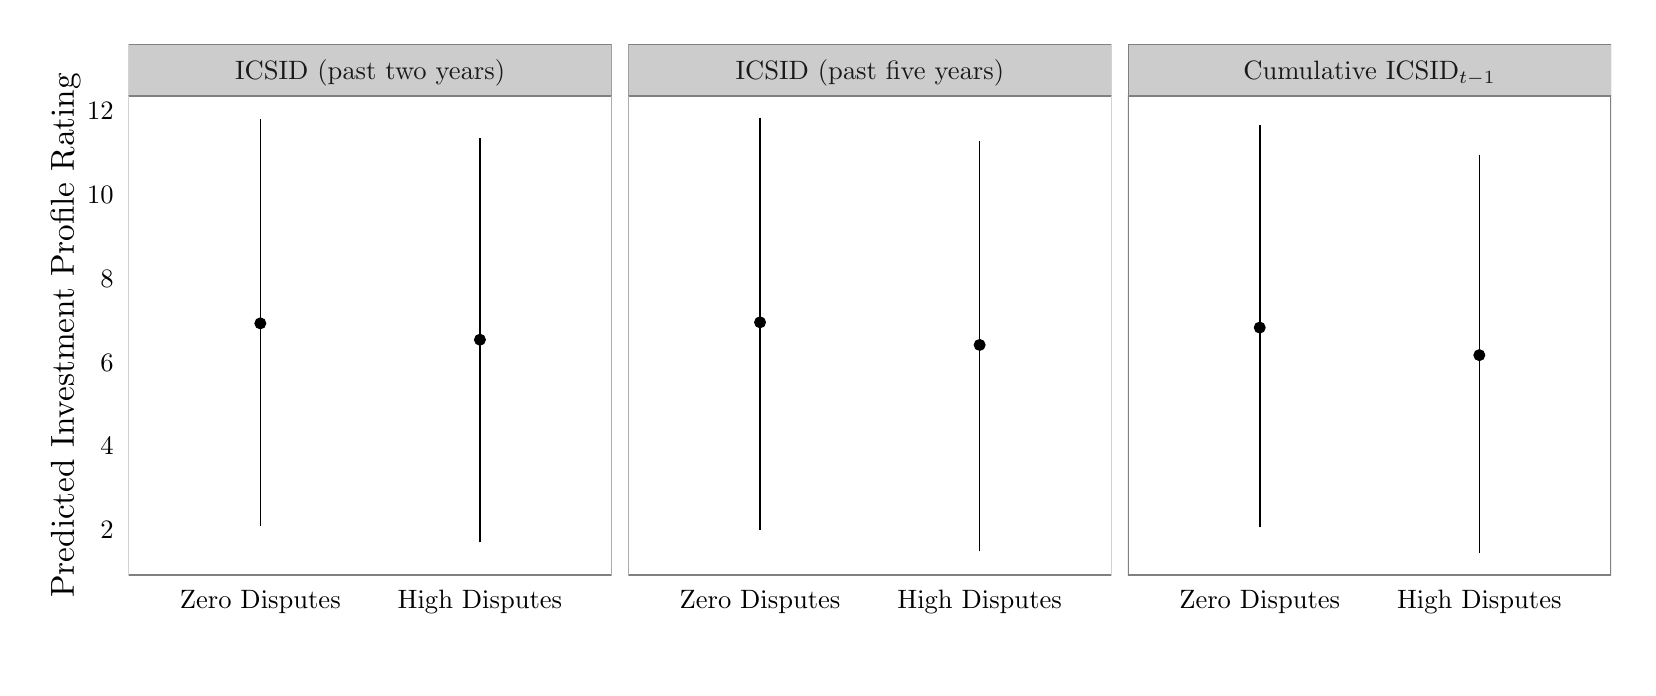
\begin{tikzpicture}[x=1pt,y=1pt]
\definecolor[named]{drawColor}{rgb}{0.00,0.00,0.00}
\definecolor[named]{fillColor}{rgb}{1.00,1.00,1.00}
\fill[color=fillColor,] (0,0) rectangle (578.16,231.26);
\begin{scope}
\path[clip] (  0.00,  0.00) rectangle (578.16,231.26);
\end{scope}
\begin{scope}
\path[clip] (  0.00,  0.00) rectangle (578.16,231.26);
\end{scope}
\begin{scope}
\path[clip] (  0.00,  0.00) rectangle (578.16,231.26);
\end{scope}
\begin{scope}
\path[clip] (  0.00,  0.00) rectangle (578.16,231.26);
\end{scope}
\begin{scope}
\path[clip] (  0.00,  0.00) rectangle (578.16,231.26);
\end{scope}
\begin{scope}
\path[clip] (  0.00,  0.00) rectangle (578.16,231.26);
\end{scope}
\begin{scope}
\path[clip] (  0.00,  0.00) rectangle (578.16,231.26);
\end{scope}
\begin{scope}
\path[clip] (  0.00,  0.00) rectangle (578.16,231.26);
\end{scope}
\begin{scope}
\path[clip] (  0.00,  0.00) rectangle (578.16,231.26);
\end{scope}
\begin{scope}
\path[clip] (  0.00,  0.00) rectangle (578.16,231.26);
\end{scope}
\begin{scope}
\path[clip] (  0.00,  0.00) rectangle (578.16,231.26);
\end{scope}
\begin{scope}
\path[clip] (  0.00,  0.00) rectangle (578.16,231.26);
\end{scope}
\begin{scope}
\path[clip] (  0.00,  0.00) rectangle (578.16,231.26);
\end{scope}
\begin{scope}
\path[clip] (  0.00,  0.00) rectangle (578.16,231.26);
\definecolor[named]{drawColor}{rgb}{1.00,1.00,1.00}
\definecolor[named]{fillColor}{rgb}{1.00,1.00,1.00}

\draw[color=drawColor,line width= 0.6pt,line cap=round,line join=round,fill=fillColor,] (  0.00,  0.00) rectangle (578.16,231.26);
\end{scope}
\begin{scope}
\path[clip] (  0.00,  0.00) rectangle (578.16,231.26);
\end{scope}
\begin{scope}
\path[clip] ( 36.46, 33.48) rectangle (211.03,206.65);
\definecolor[named]{fillColor}{rgb}{1.00,1.00,1.00}

\draw[fill=fillColor,draw opacity=0.00,] ( 36.46, 33.48) rectangle (211.03,206.65);
\definecolor[named]{drawColor}{rgb}{0.00,0.00,0.00}
\definecolor[named]{fillColor}{rgb}{0.00,0.00,0.00}

\draw[color=drawColor,line width= 0.6pt,line join=round,fill=fillColor,] ( 84.07, 51.23) -- ( 84.07,198.22);

\draw[color=drawColor,line width= 0.6pt,line join=round,fill=fillColor,] (163.42, 45.31) -- (163.42,191.56);

\draw[color=drawColor,line width= 0.4pt,line cap=round,line join=round,fill=fillColor,] ( 84.07,124.41) circle (  1.96);

\draw[color=drawColor,line width= 0.4pt,line cap=round,line join=round,fill=fillColor,] (163.42,118.50) circle (  1.96);
\definecolor[named]{drawColor}{rgb}{0.50,0.50,0.50}

\draw[color=drawColor,line width= 0.6pt,line cap=round,line join=round,fill opacity=0.00,] ( 36.46, 33.48) rectangle (211.03,206.65);
\end{scope}
\begin{scope}
\path[clip] (  0.00,  0.00) rectangle (578.16,231.26);
\end{scope}
\begin{scope}
\path[clip] (217.03, 33.48) rectangle (391.59,206.65);
\definecolor[named]{fillColor}{rgb}{1.00,1.00,1.00}

\draw[fill=fillColor,draw opacity=0.00,] (217.03, 33.48) rectangle (391.59,206.65);
\definecolor[named]{drawColor}{rgb}{0.00,0.00,0.00}
\definecolor[named]{fillColor}{rgb}{0.00,0.00,0.00}

\draw[color=drawColor,line width= 0.6pt,line join=round,fill=fillColor,] (264.64, 49.75) -- (264.64,198.78);

\draw[color=drawColor,line width= 0.6pt,line join=round,fill=fillColor,] (343.99, 42.06) -- (343.99,190.16);

\draw[color=drawColor,line width= 0.4pt,line cap=round,line join=round,fill=fillColor,] (264.64,124.79) circle (  1.96);

\draw[color=drawColor,line width= 0.4pt,line cap=round,line join=round,fill=fillColor,] (343.99,116.61) circle (  1.96);
\definecolor[named]{drawColor}{rgb}{0.50,0.50,0.50}

\draw[color=drawColor,line width= 0.6pt,line cap=round,line join=round,fill opacity=0.00,] (217.03, 33.48) rectangle (391.59,206.65);
\end{scope}
\begin{scope}
\path[clip] (  0.00,  0.00) rectangle (578.16,231.26);
\end{scope}
\begin{scope}
\path[clip] (397.59, 33.48) rectangle (572.16,206.65);
\definecolor[named]{fillColor}{rgb}{1.00,1.00,1.00}

\draw[fill=fillColor,draw opacity=0.00,] (397.59, 33.48) rectangle (572.16,206.65);
\definecolor[named]{drawColor}{rgb}{0.00,0.00,0.00}
\definecolor[named]{fillColor}{rgb}{0.00,0.00,0.00}

\draw[color=drawColor,line width= 0.6pt,line join=round,fill=fillColor,] (445.20, 50.70) -- (445.20,196.03);

\draw[color=drawColor,line width= 0.6pt,line join=round,fill=fillColor,] (524.55, 41.35) -- (524.55,185.34);

\draw[color=drawColor,line width= 0.4pt,line cap=round,line join=round,fill=fillColor,] (445.20,122.89) circle (  1.96);

\draw[color=drawColor,line width= 0.4pt,line cap=round,line join=round,fill=fillColor,] (524.55,112.93) circle (  1.96);
\definecolor[named]{drawColor}{rgb}{0.50,0.50,0.50}

\draw[color=drawColor,line width= 0.6pt,line cap=round,line join=round,fill opacity=0.00,] (397.59, 33.48) rectangle (572.16,206.65);
\end{scope}
\begin{scope}
\path[clip] (  0.00,  0.00) rectangle (578.16,231.26);
\end{scope}
\begin{scope}
\path[clip] (  0.00,  0.00) rectangle (578.16,231.26);
\end{scope}
\begin{scope}
\path[clip] (  0.00,  0.00) rectangle (578.16,231.26);
\end{scope}
\begin{scope}
\path[clip] ( 36.46,206.65) rectangle (211.03,225.26);
\definecolor[named]{drawColor}{rgb}{0.50,0.50,0.50}
\definecolor[named]{fillColor}{rgb}{0.80,0.80,0.80}

\draw[color=drawColor,line width= 0.2pt,line cap=round,line join=round,fill=fillColor,] ( 36.46,206.65) rectangle (211.03,225.26);
\definecolor[named]{drawColor}{rgb}{0.10,0.10,0.10}

\node[color=drawColor,anchor=base,inner sep=0pt, outer sep=0pt, scale=  0.96] at (123.75,212.65) {ICSID (past two years)%
};
\end{scope}
\begin{scope}
\path[clip] ( 36.46,206.65) rectangle (211.03,225.26);
\end{scope}
\begin{scope}
\path[clip] (  0.00,  0.00) rectangle (578.16,231.26);
\end{scope}
\begin{scope}
\path[clip] (  0.00,  0.00) rectangle (578.16,231.26);
\end{scope}
\begin{scope}
\path[clip] (  0.00,  0.00) rectangle (578.16,231.26);
\end{scope}
\begin{scope}
\path[clip] (  0.00,  0.00) rectangle (578.16,231.26);
\end{scope}
\begin{scope}
\path[clip] (  0.00,  0.00) rectangle (578.16,231.26);
\end{scope}
\begin{scope}
\path[clip] (  0.00,  0.00) rectangle (578.16,231.26);
\end{scope}
\begin{scope}
\path[clip] (217.03,206.65) rectangle (391.59,225.26);
\definecolor[named]{drawColor}{rgb}{0.50,0.50,0.50}
\definecolor[named]{fillColor}{rgb}{0.80,0.80,0.80}

\draw[color=drawColor,line width= 0.2pt,line cap=round,line join=round,fill=fillColor,] (217.03,206.65) rectangle (391.59,225.26);
\definecolor[named]{drawColor}{rgb}{0.10,0.10,0.10}

\node[color=drawColor,anchor=base,inner sep=0pt, outer sep=0pt, scale=  0.96] at (304.31,212.65) {ICSID (past five years)%
};
\end{scope}
\begin{scope}
\path[clip] (217.03,206.65) rectangle (391.59,225.26);
\end{scope}
\begin{scope}
\path[clip] (  0.00,  0.00) rectangle (578.16,231.26);
\end{scope}
\begin{scope}
\path[clip] (  0.00,  0.00) rectangle (578.16,231.26);
\end{scope}
\begin{scope}
\path[clip] (  0.00,  0.00) rectangle (578.16,231.26);
\end{scope}
\begin{scope}
\path[clip] (  0.00,  0.00) rectangle (578.16,231.26);
\end{scope}
\begin{scope}
\path[clip] (  0.00,  0.00) rectangle (578.16,231.26);
\end{scope}
\begin{scope}
\path[clip] (  0.00,  0.00) rectangle (578.16,231.26);
\end{scope}
\begin{scope}
\path[clip] (397.59,206.65) rectangle (572.16,225.26);
\definecolor[named]{drawColor}{rgb}{0.50,0.50,0.50}
\definecolor[named]{fillColor}{rgb}{0.80,0.80,0.80}

\draw[color=drawColor,line width= 0.2pt,line cap=round,line join=round,fill=fillColor,] (397.59,206.65) rectangle (572.16,225.26);
\definecolor[named]{drawColor}{rgb}{0.10,0.10,0.10}

\node[color=drawColor,anchor=base,inner sep=0pt, outer sep=0pt, scale=  0.96] at (484.88,212.65) {Cumulative ICSID$_{t-1}$%
};
\end{scope}
\begin{scope}
\path[clip] (397.59,206.65) rectangle (572.16,225.26);
\end{scope}
\begin{scope}
\path[clip] (  0.00,  0.00) rectangle (578.16,231.26);
\end{scope}
\begin{scope}
\path[clip] (  0.00,  0.00) rectangle (578.16,231.26);
\end{scope}
\begin{scope}
\path[clip] (  0.00,  0.00) rectangle (578.16,231.26);
\end{scope}
\begin{scope}
\path[clip] (  0.00,  0.00) rectangle (578.16,231.26);
\end{scope}
\begin{scope}
\path[clip] (  0.00,  0.00) rectangle (578.16,231.26);
\end{scope}
\begin{scope}
\path[clip] (  0.00,  0.00) rectangle (578.16,231.26);
\end{scope}
\begin{scope}
\path[clip] (  0.00,  0.00) rectangle (578.16,231.26);
\end{scope}
\begin{scope}
\path[clip] (  0.00,  0.00) rectangle (578.16,231.26);
\end{scope}
\begin{scope}
\path[clip] (  0.00,  0.00) rectangle (578.16,231.26);
\definecolor[named]{drawColor}{rgb}{0.00,0.00,0.00}

\node[color=drawColor,anchor=base east,inner sep=0pt, outer sep=0pt, scale=  0.96] at ( 31.06, 46.57) {2%
};

\node[color=drawColor,anchor=base east,inner sep=0pt, outer sep=0pt, scale=  0.96] at ( 31.06, 76.85) {4%
};

\node[color=drawColor,anchor=base east,inner sep=0pt, outer sep=0pt, scale=  0.96] at ( 31.06,107.14) {6%
};

\node[color=drawColor,anchor=base east,inner sep=0pt, outer sep=0pt, scale=  0.96] at ( 31.06,137.42) {8%
};

\node[color=drawColor,anchor=base east,inner sep=0pt, outer sep=0pt, scale=  0.96] at ( 31.06,167.70) {10%
};

\node[color=drawColor,anchor=base east,inner sep=0pt, outer sep=0pt, scale=  0.96] at ( 31.06,197.98) {12%
};
\end{scope}
\begin{scope}
\path[clip] (  0.00,  0.00) rectangle (578.16,231.26);
\end{scope}
\begin{scope}
\path[clip] (  0.00,  0.00) rectangle (578.16,231.26);
\end{scope}
\begin{scope}
\path[clip] (  0.00,  0.00) rectangle (578.16,231.26);
\end{scope}
\begin{scope}
\path[clip] (  0.00,  0.00) rectangle (578.16,231.26);
\end{scope}
\begin{scope}
\path[clip] (  0.00,  0.00) rectangle (578.16,231.26);
\end{scope}
\begin{scope}
\path[clip] (  0.00,  0.00) rectangle (578.16,231.26);
\end{scope}
\begin{scope}
\path[clip] (  0.00,  0.00) rectangle (578.16,231.26);
\end{scope}
\begin{scope}
\path[clip] (  0.00,  0.00) rectangle (578.16,231.26);
\end{scope}
\begin{scope}
\path[clip] (  0.00,  0.00) rectangle (578.16,231.26);
\end{scope}
\begin{scope}
\path[clip] (  0.00,  0.00) rectangle (578.16,231.26);
\end{scope}
\begin{scope}
\path[clip] (  0.00,  0.00) rectangle (578.16,231.26);
\end{scope}
\begin{scope}
\path[clip] (  0.00,  0.00) rectangle (578.16,231.26);
\end{scope}
\begin{scope}
\path[clip] (  0.00,  0.00) rectangle (578.16,231.26);
\end{scope}
\begin{scope}
\path[clip] (  0.00,  0.00) rectangle (578.16,231.26);
\end{scope}
\begin{scope}
\path[clip] (  0.00,  0.00) rectangle (578.16,231.26);
\end{scope}
\begin{scope}
\path[clip] (  0.00,  0.00) rectangle (578.16,231.26);
\end{scope}
\begin{scope}
\path[clip] (  0.00,  0.00) rectangle (578.16,231.26);
\end{scope}
\begin{scope}
\path[clip] (  0.00,  0.00) rectangle (578.16,231.26);
\definecolor[named]{drawColor}{rgb}{0.00,0.00,0.00}

\node[color=drawColor,anchor=base,inner sep=0pt, outer sep=0pt, scale=  0.96] at ( 84.07, 21.46) {Zero Disputes%
};

\node[color=drawColor,anchor=base,inner sep=0pt, outer sep=0pt, scale=  0.96] at (163.42, 21.46) {High Disputes%
};
\end{scope}
\begin{scope}
\path[clip] (  0.00,  0.00) rectangle (578.16,231.26);
\end{scope}
\begin{scope}
\path[clip] (  0.00,  0.00) rectangle (578.16,231.26);
\end{scope}
\begin{scope}
\path[clip] (  0.00,  0.00) rectangle (578.16,231.26);
\end{scope}
\begin{scope}
\path[clip] (  0.00,  0.00) rectangle (578.16,231.26);
\end{scope}
\begin{scope}
\path[clip] (  0.00,  0.00) rectangle (578.16,231.26);
\end{scope}
\begin{scope}
\path[clip] (  0.00,  0.00) rectangle (578.16,231.26);
\end{scope}
\begin{scope}
\path[clip] (  0.00,  0.00) rectangle (578.16,231.26);
\end{scope}
\begin{scope}
\path[clip] (  0.00,  0.00) rectangle (578.16,231.26);
\end{scope}
\begin{scope}
\path[clip] (  0.00,  0.00) rectangle (578.16,231.26);
\end{scope}
\begin{scope}
\path[clip] (  0.00,  0.00) rectangle (578.16,231.26);
\end{scope}
\begin{scope}
\path[clip] (  0.00,  0.00) rectangle (578.16,231.26);
\end{scope}
\begin{scope}
\path[clip] (  0.00,  0.00) rectangle (578.16,231.26);
\definecolor[named]{drawColor}{rgb}{0.00,0.00,0.00}

\node[color=drawColor,anchor=base,inner sep=0pt, outer sep=0pt, scale=  0.96] at (264.64, 21.46) {Zero Disputes%
};

\node[color=drawColor,anchor=base,inner sep=0pt, outer sep=0pt, scale=  0.96] at (343.99, 21.46) {High Disputes%
};
\end{scope}
\begin{scope}
\path[clip] (  0.00,  0.00) rectangle (578.16,231.26);
\end{scope}
\begin{scope}
\path[clip] (  0.00,  0.00) rectangle (578.16,231.26);
\end{scope}
\begin{scope}
\path[clip] (  0.00,  0.00) rectangle (578.16,231.26);
\end{scope}
\begin{scope}
\path[clip] (  0.00,  0.00) rectangle (578.16,231.26);
\end{scope}
\begin{scope}
\path[clip] (  0.00,  0.00) rectangle (578.16,231.26);
\end{scope}
\begin{scope}
\path[clip] (  0.00,  0.00) rectangle (578.16,231.26);
\end{scope}
\begin{scope}
\path[clip] (  0.00,  0.00) rectangle (578.16,231.26);
\end{scope}
\begin{scope}
\path[clip] (  0.00,  0.00) rectangle (578.16,231.26);
\end{scope}
\begin{scope}
\path[clip] (  0.00,  0.00) rectangle (578.16,231.26);
\end{scope}
\begin{scope}
\path[clip] (  0.00,  0.00) rectangle (578.16,231.26);
\end{scope}
\begin{scope}
\path[clip] (  0.00,  0.00) rectangle (578.16,231.26);
\end{scope}
\begin{scope}
\path[clip] (  0.00,  0.00) rectangle (578.16,231.26);
\definecolor[named]{drawColor}{rgb}{0.00,0.00,0.00}

\node[color=drawColor,anchor=base,inner sep=0pt, outer sep=0pt, scale=  0.96] at (445.20, 21.46) {Zero Disputes%
};

\node[color=drawColor,anchor=base,inner sep=0pt, outer sep=0pt, scale=  0.96] at (524.55, 21.46) {High Disputes%
};
\end{scope}
\begin{scope}
\path[clip] (  0.00,  0.00) rectangle (578.16,231.26);
\end{scope}
\begin{scope}
\path[clip] (  0.00,  0.00) rectangle (578.16,231.26);
\end{scope}
\begin{scope}
\path[clip] (  0.00,  0.00) rectangle (578.16,231.26);
\end{scope}
\begin{scope}
\path[clip] (  0.00,  0.00) rectangle (578.16,231.26);
\end{scope}
\begin{scope}
\path[clip] (  0.00,  0.00) rectangle (578.16,231.26);
\end{scope}
\begin{scope}
\path[clip] (  0.00,  0.00) rectangle (578.16,231.26);
\end{scope}
\begin{scope}
\path[clip] (  0.00,  0.00) rectangle (578.16,231.26);
\end{scope}
\begin{scope}
\path[clip] (  0.00,  0.00) rectangle (578.16,231.26);
\end{scope}
\begin{scope}
\path[clip] (  0.00,  0.00) rectangle (578.16,231.26);
\definecolor[named]{drawColor}{rgb}{0.00,0.00,0.00}

\node[rotate= 90.00,color=drawColor,anchor=base,inner sep=0pt, outer sep=0pt, scale=  1.20] at ( 16.66,120.06) {Predicted Investment Profile Rating%
};
\end{scope}
\begin{scope}
\path[clip] (  0.00,  0.00) rectangle (578.16,231.26);
\end{scope}
\begin{scope}
\path[clip] (  0.00,  0.00) rectangle (578.16,231.26);
\end{scope}
\begin{scope}
\path[clip] (  0.00,  0.00) rectangle (578.16,231.26);
\end{scope}
\begin{scope}
\path[clip] (  0.00,  0.00) rectangle (578.16,231.26);
\end{scope}
\begin{scope}
\path[clip] (  0.00,  0.00) rectangle (578.16,231.26);
\end{scope}
\end{tikzpicture}
}	
\end{figure}

\end{frame}
%%%%%%%%%%%%%%%%%%%%%%%%%%%%%%%%%%%%%%%%%

%%%%%%%%%%%%%%%%%%%%%%%%%%%%%%%%%%%%%%%%%
\begin{frame}
\frametitle{Change over Disputes Over Time}

\begin{figure}[ht]
	\centering
	\resizebox{1\textwidth}{!}{% Created by tikzDevice version 0.7.0 on 2015-01-23 00:08:45
% !TEX encoding = UTF-8 Unicode
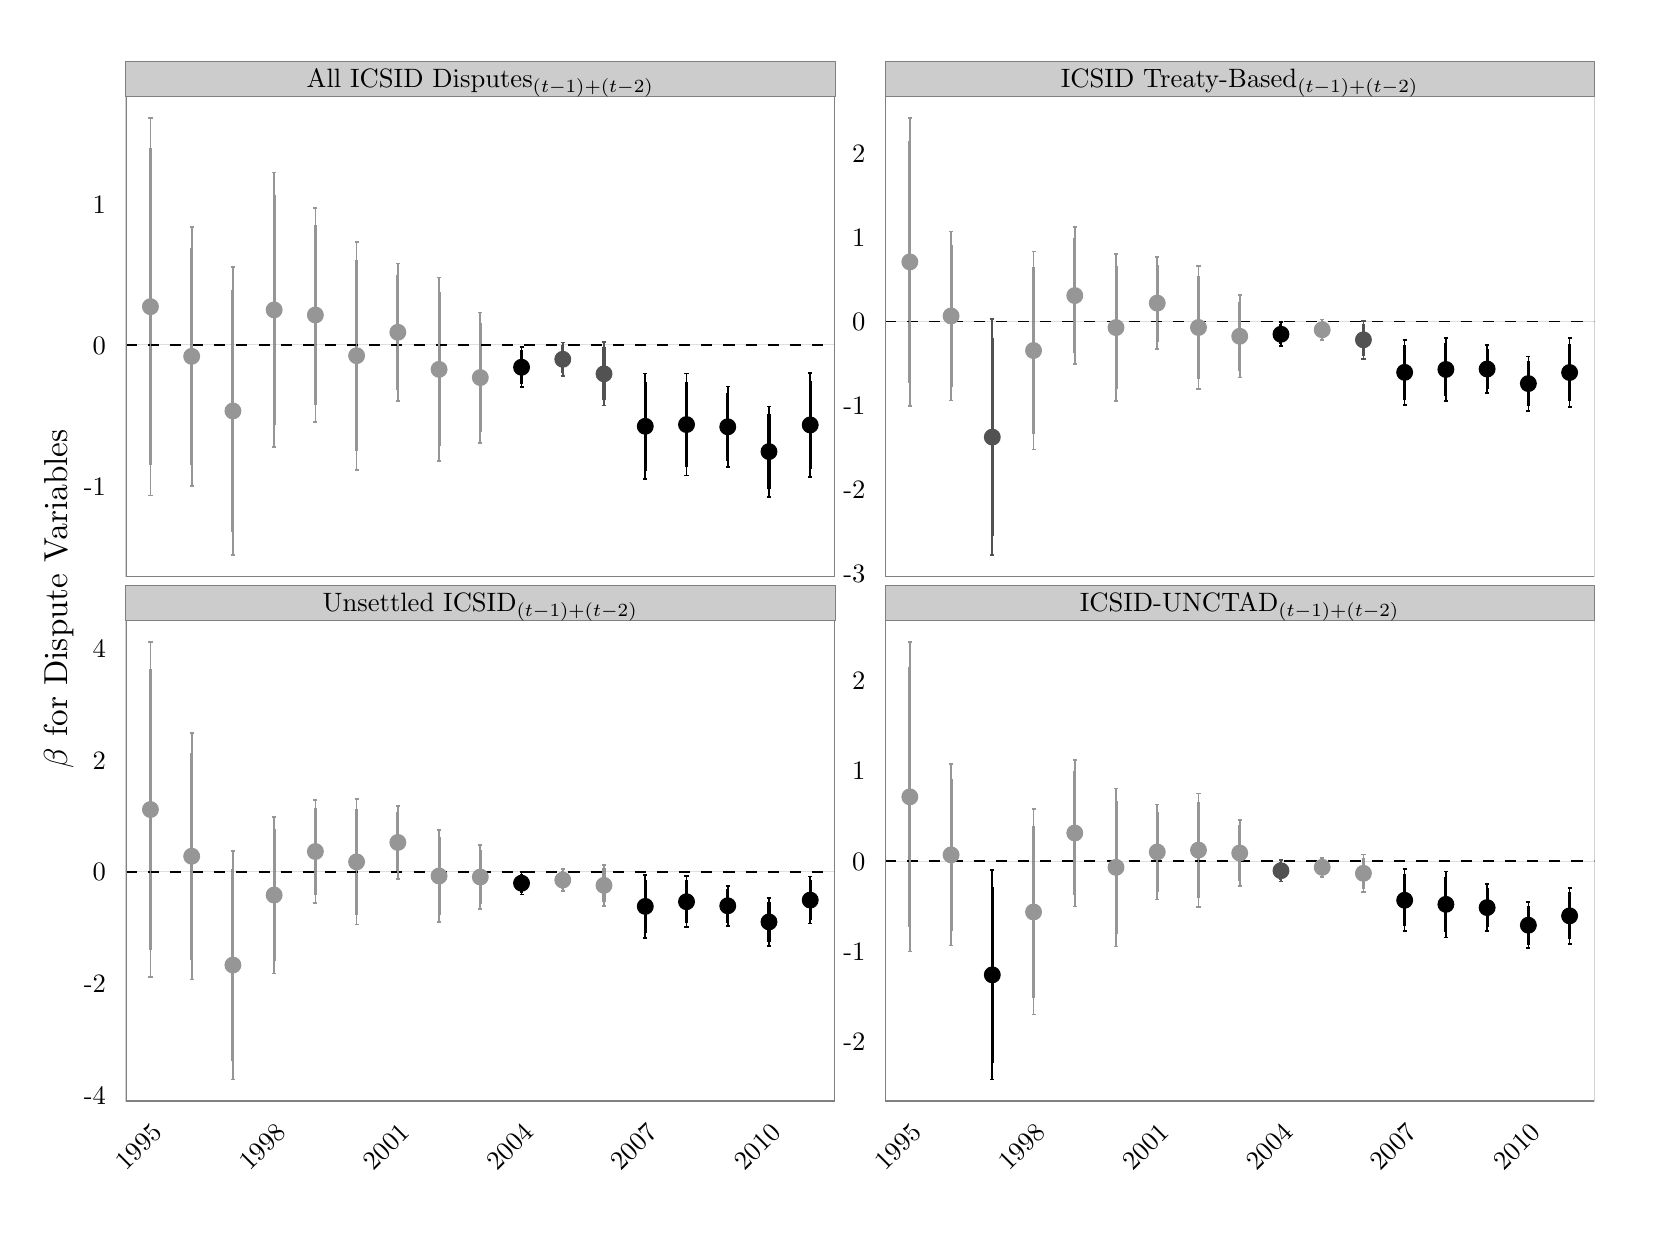
\begin{tikzpicture}[x=1pt,y=1pt]
\definecolor[named]{fillColor}{rgb}{1.00,1.00,1.00}
\path[use as bounding box,fill=fillColor,fill opacity=0.00] (0,0) rectangle (578.16,433.62);
\begin{scope}
\path[clip] (  0.00,  0.00) rectangle (578.16,433.62);
\definecolor[named]{drawColor}{rgb}{1.00,1.00,1.00}
\definecolor[named]{fillColor}{rgb}{1.00,1.00,1.00}

\path[draw=drawColor,line width= 0.6pt,line join=round,line cap=round,fill=fillColor] (  0.00,  0.00) rectangle (578.16,433.62);
\end{scope}
\begin{scope}
\path[clip] ( 35.42,235.13) rectangle (291.71,408.94);
\definecolor[named]{fillColor}{rgb}{1.00,1.00,1.00}

\path[fill=fillColor] ( 35.42,235.13) rectangle (291.71,408.94);
\definecolor[named]{drawColor}{rgb}{0.59,0.59,0.59}
\definecolor[named]{fillColor}{rgb}{0.59,0.59,0.59}

\path[draw=drawColor,draw opacity=0.30,line width= 0.3pt,line join=round,fill=fillColor,fill opacity=0.30] ( 44.36,264.57) -- ( 44.36,401.04);

\path[draw=drawColor,draw opacity=0.30,line width= 0.3pt,line join=round,fill=fillColor,fill opacity=0.30] ( 59.26,268.08) -- ( 59.26,361.64);

\path[draw=drawColor,draw opacity=0.30,line width= 0.3pt,line join=round,fill=fillColor,fill opacity=0.30] ( 74.16,243.03) -- ( 74.16,347.20);

\path[draw=drawColor,draw opacity=0.30,line width= 0.3pt,line join=round,fill=fillColor,fill opacity=0.30] ( 89.06,282.03) -- ( 89.06,381.24);

\path[draw=drawColor,draw opacity=0.30,line width= 0.3pt,line join=round,fill=fillColor,fill opacity=0.30] (103.96,291.12) -- (103.96,368.46);

\path[draw=drawColor,draw opacity=0.30,line width= 0.3pt,line join=round,fill=fillColor,fill opacity=0.30] (118.86,273.90) -- (118.86,356.28);

\path[draw=drawColor,draw opacity=0.30,line width= 0.3pt,line join=round,fill=fillColor,fill opacity=0.30] (133.76,298.70) -- (133.76,348.40);

\path[draw=drawColor,draw opacity=0.30,line width= 0.3pt,line join=round,fill=fillColor,fill opacity=0.30] (148.66,276.98) -- (148.66,343.29);

\path[draw=drawColor,draw opacity=0.30,line width= 0.3pt,line join=round,fill=fillColor,fill opacity=0.30] (163.56,283.63) -- (163.56,330.74);
\definecolor[named]{drawColor}{rgb}{0.00,0.00,0.00}
\definecolor[named]{fillColor}{rgb}{0.00,0.00,0.00}

\path[draw=drawColor,draw opacity=0.30,line width= 0.3pt,line join=round,fill=fillColor,fill opacity=0.30] (178.46,303.67) -- (178.46,318.14);
\definecolor[named]{drawColor}{rgb}{0.32,0.32,0.32}
\definecolor[named]{fillColor}{rgb}{0.32,0.32,0.32}

\path[draw=drawColor,draw opacity=0.30,line width= 0.3pt,line join=round,fill=fillColor,fill opacity=0.30] (193.36,307.68) -- (193.36,319.90);

\path[draw=drawColor,draw opacity=0.30,line width= 0.3pt,line join=round,fill=fillColor,fill opacity=0.30] (208.26,297.13) -- (208.26,319.93);
\definecolor[named]{drawColor}{rgb}{0.00,0.00,0.00}
\definecolor[named]{fillColor}{rgb}{0.00,0.00,0.00}

\path[draw=drawColor,draw opacity=0.30,line width= 0.3pt,line join=round,fill=fillColor,fill opacity=0.30] (223.17,270.42) -- (223.17,308.71);

\path[draw=drawColor,draw opacity=0.30,line width= 0.3pt,line join=round,fill=fillColor,fill opacity=0.30] (238.07,271.74) -- (238.07,308.67);

\path[draw=drawColor,draw opacity=0.30,line width= 0.3pt,line join=round,fill=fillColor,fill opacity=0.30] (252.97,274.84) -- (252.97,303.93);

\path[draw=drawColor,draw opacity=0.30,line width= 0.3pt,line join=round,fill=fillColor,fill opacity=0.30] (267.87,264.12) -- (267.87,296.74);

\path[draw=drawColor,draw opacity=0.30,line width= 0.3pt,line join=round,fill=fillColor,fill opacity=0.30] (282.77,271.21) -- (282.77,308.92);
\definecolor[named]{drawColor}{rgb}{0.59,0.59,0.59}
\definecolor[named]{fillColor}{rgb}{0.59,0.59,0.59}

\path[draw=drawColor,line width= 1.1pt,line join=round,fill=fillColor] ( 44.36,275.54) -- ( 44.36,390.07);

\path[draw=drawColor,line width= 1.1pt,line join=round,fill=fillColor] ( 59.26,275.60) -- ( 59.26,354.12);

\path[draw=drawColor,line width= 1.1pt,line join=round,fill=fillColor] ( 74.16,251.40) -- ( 74.16,338.82);

\path[draw=drawColor,line width= 1.1pt,line join=round,fill=fillColor] ( 89.06,290.00) -- ( 89.06,373.26);

\path[draw=drawColor,line width= 1.1pt,line join=round,fill=fillColor] (103.96,297.34) -- (103.96,362.24);

\path[draw=drawColor,line width= 1.1pt,line join=round,fill=fillColor] (118.86,280.52) -- (118.86,349.65);

\path[draw=drawColor,line width= 1.1pt,line join=round,fill=fillColor] (133.76,302.70) -- (133.76,344.41);

\path[draw=drawColor,line width= 1.1pt,line join=round,fill=fillColor] (148.66,282.31) -- (148.66,337.96);

\path[draw=drawColor,line width= 1.1pt,line join=round,fill=fillColor] (163.56,287.42) -- (163.56,326.95);
\definecolor[named]{drawColor}{rgb}{0.00,0.00,0.00}
\definecolor[named]{fillColor}{rgb}{0.00,0.00,0.00}

\path[draw=drawColor,line width= 1.1pt,line join=round,fill=fillColor] (178.46,304.83) -- (178.46,316.98);
\definecolor[named]{drawColor}{rgb}{0.32,0.32,0.32}
\definecolor[named]{fillColor}{rgb}{0.32,0.32,0.32}

\path[draw=drawColor,line width= 1.1pt,line join=round,fill=fillColor] (193.36,308.66) -- (193.36,318.92);

\path[draw=drawColor,line width= 1.1pt,line join=round,fill=fillColor] (208.26,298.97) -- (208.26,318.10);
\definecolor[named]{drawColor}{rgb}{0.00,0.00,0.00}
\definecolor[named]{fillColor}{rgb}{0.00,0.00,0.00}

\path[draw=drawColor,line width= 1.1pt,line join=round,fill=fillColor] (223.17,273.50) -- (223.17,305.63);

\path[draw=drawColor,line width= 1.1pt,line join=round,fill=fillColor] (238.07,274.71) -- (238.07,305.70);

\path[draw=drawColor,line width= 1.1pt,line join=round,fill=fillColor] (252.97,277.18) -- (252.97,301.59);

\path[draw=drawColor,line width= 1.1pt,line join=round,fill=fillColor] (267.87,266.74) -- (267.87,294.12);

\path[draw=drawColor,line width= 1.1pt,line join=round,fill=fillColor] (282.77,274.24) -- (282.77,305.89);

\path[draw=drawColor,line width= 0.6pt,dash pattern=on 4pt off 4pt ,line join=round,fill=fillColor] ( 35.42,318.97) -- (291.71,318.97);
\definecolor[named]{drawColor}{rgb}{0.59,0.59,0.59}
\definecolor[named]{fillColor}{rgb}{0.59,0.59,0.59}

\path[draw=drawColor,line width= 0.4pt,line join=round,line cap=round,fill=fillColor] ( 44.36,332.80) circle (  2.85);

\path[draw=drawColor,line width= 0.4pt,line join=round,line cap=round,fill=fillColor] ( 59.26,314.86) circle (  2.85);

\path[draw=drawColor,line width= 0.4pt,line join=round,line cap=round,fill=fillColor] ( 74.16,295.11) circle (  2.85);

\path[draw=drawColor,line width= 0.4pt,line join=round,line cap=round,fill=fillColor] ( 89.06,331.63) circle (  2.85);

\path[draw=drawColor,line width= 0.4pt,line join=round,line cap=round,fill=fillColor] (103.96,329.79) circle (  2.85);

\path[draw=drawColor,line width= 0.4pt,line join=round,line cap=round,fill=fillColor] (118.86,315.09) circle (  2.85);

\path[draw=drawColor,line width= 0.4pt,line join=round,line cap=round,fill=fillColor] (133.76,323.55) circle (  2.85);

\path[draw=drawColor,line width= 0.4pt,line join=round,line cap=round,fill=fillColor] (148.66,310.14) circle (  2.85);

\path[draw=drawColor,line width= 0.4pt,line join=round,line cap=round,fill=fillColor] (163.56,307.18) circle (  2.85);
\definecolor[named]{drawColor}{rgb}{0.00,0.00,0.00}
\definecolor[named]{fillColor}{rgb}{0.00,0.00,0.00}

\path[draw=drawColor,line width= 0.4pt,line join=round,line cap=round,fill=fillColor] (178.46,310.91) circle (  2.85);
\definecolor[named]{drawColor}{rgb}{0.32,0.32,0.32}
\definecolor[named]{fillColor}{rgb}{0.32,0.32,0.32}

\path[draw=drawColor,line width= 0.4pt,line join=round,line cap=round,fill=fillColor] (193.36,313.79) circle (  2.85);

\path[draw=drawColor,line width= 0.4pt,line join=round,line cap=round,fill=fillColor] (208.26,308.53) circle (  2.85);
\definecolor[named]{drawColor}{rgb}{0.00,0.00,0.00}
\definecolor[named]{fillColor}{rgb}{0.00,0.00,0.00}

\path[draw=drawColor,line width= 0.4pt,line join=round,line cap=round,fill=fillColor] (223.17,289.57) circle (  2.85);

\path[draw=drawColor,line width= 0.4pt,line join=round,line cap=round,fill=fillColor] (238.07,290.20) circle (  2.85);

\path[draw=drawColor,line width= 0.4pt,line join=round,line cap=round,fill=fillColor] (252.97,289.39) circle (  2.85);

\path[draw=drawColor,line width= 0.4pt,line join=round,line cap=round,fill=fillColor] (267.87,280.43) circle (  2.85);

\path[draw=drawColor,line width= 0.4pt,line join=round,line cap=round,fill=fillColor] (282.77,290.06) circle (  2.85);
\definecolor[named]{drawColor}{rgb}{0.59,0.59,0.59}

\path[draw=drawColor,line width= 0.6pt,line join=round] ( 43.62,401.04) --
	( 45.11,401.04);

\path[draw=drawColor,line width= 0.6pt,line join=round] ( 44.36,401.04) --
	( 44.36,264.57);

\path[draw=drawColor,line width= 0.6pt,line join=round] ( 43.62,264.57) --
	( 45.11,264.57);

\path[draw=drawColor,line width= 0.6pt,line join=round] ( 58.52,361.64) --
	( 60.01,361.64);

\path[draw=drawColor,line width= 0.6pt,line join=round] ( 59.26,361.64) --
	( 59.26,268.08);

\path[draw=drawColor,line width= 0.6pt,line join=round] ( 58.52,268.08) --
	( 60.01,268.08);

\path[draw=drawColor,line width= 0.6pt,line join=round] ( 73.42,347.20) --
	( 74.91,347.20);

\path[draw=drawColor,line width= 0.6pt,line join=round] ( 74.16,347.20) --
	( 74.16,243.03);

\path[draw=drawColor,line width= 0.6pt,line join=round] ( 73.42,243.03) --
	( 74.91,243.03);

\path[draw=drawColor,line width= 0.6pt,line join=round] ( 88.32,381.24) --
	( 89.81,381.24);

\path[draw=drawColor,line width= 0.6pt,line join=round] ( 89.06,381.24) --
	( 89.06,282.03);

\path[draw=drawColor,line width= 0.6pt,line join=round] ( 88.32,282.03) --
	( 89.81,282.03);

\path[draw=drawColor,line width= 0.6pt,line join=round] (103.22,368.46) --
	(104.71,368.46);

\path[draw=drawColor,line width= 0.6pt,line join=round] (103.96,368.46) --
	(103.96,291.12);

\path[draw=drawColor,line width= 0.6pt,line join=round] (103.22,291.12) --
	(104.71,291.12);

\path[draw=drawColor,line width= 0.6pt,line join=round] (118.12,356.28) --
	(119.61,356.28);

\path[draw=drawColor,line width= 0.6pt,line join=round] (118.86,356.28) --
	(118.86,273.90);

\path[draw=drawColor,line width= 0.6pt,line join=round] (118.12,273.90) --
	(119.61,273.90);

\path[draw=drawColor,line width= 0.6pt,line join=round] (133.02,348.40) --
	(134.51,348.40);

\path[draw=drawColor,line width= 0.6pt,line join=round] (133.76,348.40) --
	(133.76,298.70);

\path[draw=drawColor,line width= 0.6pt,line join=round] (133.02,298.70) --
	(134.51,298.70);

\path[draw=drawColor,line width= 0.6pt,line join=round] (147.92,343.29) --
	(149.41,343.29);

\path[draw=drawColor,line width= 0.6pt,line join=round] (148.66,343.29) --
	(148.66,276.98);

\path[draw=drawColor,line width= 0.6pt,line join=round] (147.92,276.98) --
	(149.41,276.98);

\path[draw=drawColor,line width= 0.6pt,line join=round] (162.82,330.74) --
	(164.31,330.74);

\path[draw=drawColor,line width= 0.6pt,line join=round] (163.56,330.74) --
	(163.56,283.63);

\path[draw=drawColor,line width= 0.6pt,line join=round] (162.82,283.63) --
	(164.31,283.63);
\definecolor[named]{drawColor}{rgb}{0.00,0.00,0.00}

\path[draw=drawColor,line width= 0.6pt,line join=round] (177.72,318.14) --
	(179.21,318.14);

\path[draw=drawColor,line width= 0.6pt,line join=round] (178.46,318.14) --
	(178.46,303.67);

\path[draw=drawColor,line width= 0.6pt,line join=round] (177.72,303.67) --
	(179.21,303.67);
\definecolor[named]{drawColor}{rgb}{0.32,0.32,0.32}

\path[draw=drawColor,line width= 0.6pt,line join=round] (192.62,319.90) --
	(194.11,319.90);

\path[draw=drawColor,line width= 0.6pt,line join=round] (193.36,319.90) --
	(193.36,307.68);

\path[draw=drawColor,line width= 0.6pt,line join=round] (192.62,307.68) --
	(194.11,307.68);

\path[draw=drawColor,line width= 0.6pt,line join=round] (207.52,319.93) --
	(209.01,319.93);

\path[draw=drawColor,line width= 0.6pt,line join=round] (208.26,319.93) --
	(208.26,297.13);

\path[draw=drawColor,line width= 0.6pt,line join=round] (207.52,297.13) --
	(209.01,297.13);
\definecolor[named]{drawColor}{rgb}{0.00,0.00,0.00}

\path[draw=drawColor,line width= 0.6pt,line join=round] (222.42,308.71) --
	(223.91,308.71);

\path[draw=drawColor,line width= 0.6pt,line join=round] (223.17,308.71) --
	(223.17,270.42);

\path[draw=drawColor,line width= 0.6pt,line join=round] (222.42,270.42) --
	(223.91,270.42);

\path[draw=drawColor,line width= 0.6pt,line join=round] (237.32,308.67) --
	(238.81,308.67);

\path[draw=drawColor,line width= 0.6pt,line join=round] (238.07,308.67) --
	(238.07,271.74);

\path[draw=drawColor,line width= 0.6pt,line join=round] (237.32,271.74) --
	(238.81,271.74);

\path[draw=drawColor,line width= 0.6pt,line join=round] (252.22,303.93) --
	(253.71,303.93);

\path[draw=drawColor,line width= 0.6pt,line join=round] (252.97,303.93) --
	(252.97,274.84);

\path[draw=drawColor,line width= 0.6pt,line join=round] (252.22,274.84) --
	(253.71,274.84);

\path[draw=drawColor,line width= 0.6pt,line join=round] (267.12,296.74) --
	(268.61,296.74);

\path[draw=drawColor,line width= 0.6pt,line join=round] (267.87,296.74) --
	(267.87,264.12);

\path[draw=drawColor,line width= 0.6pt,line join=round] (267.12,264.12) --
	(268.61,264.12);

\path[draw=drawColor,line width= 0.6pt,line join=round] (282.02,308.92) --
	(283.51,308.92);

\path[draw=drawColor,line width= 0.6pt,line join=round] (282.77,308.92) --
	(282.77,271.21);

\path[draw=drawColor,line width= 0.6pt,line join=round] (282.02,271.21) --
	(283.51,271.21);
\definecolor[named]{drawColor}{rgb}{0.50,0.50,0.50}

\path[draw=drawColor,line width= 0.6pt,line join=round,line cap=round] ( 35.42,235.13) rectangle (291.71,408.94);
\end{scope}
\begin{scope}
\path[clip] (309.83,235.13) rectangle (566.12,408.94);
\definecolor[named]{fillColor}{rgb}{1.00,1.00,1.00}

\path[fill=fillColor] (309.83,235.13) rectangle (566.12,408.94);
\definecolor[named]{drawColor}{rgb}{0.59,0.59,0.59}
\definecolor[named]{fillColor}{rgb}{0.59,0.59,0.59}

\path[draw=drawColor,draw opacity=0.30,line width= 0.3pt,line join=round,fill=fillColor,fill opacity=0.30] (318.77,296.91) -- (318.77,401.04);

\path[draw=drawColor,draw opacity=0.30,line width= 0.3pt,line join=round,fill=fillColor,fill opacity=0.30] (333.67,298.91) -- (333.67,359.98);
\definecolor[named]{drawColor}{rgb}{0.32,0.32,0.32}
\definecolor[named]{fillColor}{rgb}{0.32,0.32,0.32}

\path[draw=drawColor,draw opacity=0.30,line width= 0.3pt,line join=round,fill=fillColor,fill opacity=0.30] (348.57,243.03) -- (348.57,328.29);
\definecolor[named]{drawColor}{rgb}{0.59,0.59,0.59}
\definecolor[named]{fillColor}{rgb}{0.59,0.59,0.59}

\path[draw=drawColor,draw opacity=0.30,line width= 0.3pt,line join=round,fill=fillColor,fill opacity=0.30] (363.47,281.18) -- (363.47,352.72);

\path[draw=drawColor,draw opacity=0.30,line width= 0.3pt,line join=round,fill=fillColor,fill opacity=0.30] (378.37,312.13) -- (378.37,361.49);

\path[draw=drawColor,draw opacity=0.30,line width= 0.3pt,line join=round,fill=fillColor,fill opacity=0.30] (393.27,298.64) -- (393.27,351.85);

\path[draw=drawColor,draw opacity=0.30,line width= 0.3pt,line join=round,fill=fillColor,fill opacity=0.30] (408.17,317.52) -- (408.17,350.65);

\path[draw=drawColor,draw opacity=0.30,line width= 0.3pt,line join=round,fill=fillColor,fill opacity=0.30] (423.07,302.98) -- (423.07,347.58);

\path[draw=drawColor,draw opacity=0.30,line width= 0.3pt,line join=round,fill=fillColor,fill opacity=0.30] (437.97,307.17) -- (437.97,337.03);
\definecolor[named]{drawColor}{rgb}{0.00,0.00,0.00}
\definecolor[named]{fillColor}{rgb}{0.00,0.00,0.00}

\path[draw=drawColor,draw opacity=0.30,line width= 0.3pt,line join=round,fill=fillColor,fill opacity=0.30] (452.87,318.49) -- (452.87,327.17);
\definecolor[named]{drawColor}{rgb}{0.59,0.59,0.59}
\definecolor[named]{fillColor}{rgb}{0.59,0.59,0.59}

\path[draw=drawColor,draw opacity=0.30,line width= 0.3pt,line join=round,fill=fillColor,fill opacity=0.30] (467.77,320.78) -- (467.77,328.11);
\definecolor[named]{drawColor}{rgb}{0.32,0.32,0.32}
\definecolor[named]{fillColor}{rgb}{0.32,0.32,0.32}

\path[draw=drawColor,draw opacity=0.30,line width= 0.3pt,line join=round,fill=fillColor,fill opacity=0.30] (482.67,313.93) -- (482.67,327.71);
\definecolor[named]{drawColor}{rgb}{0.00,0.00,0.00}
\definecolor[named]{fillColor}{rgb}{0.00,0.00,0.00}

\path[draw=drawColor,draw opacity=0.30,line width= 0.3pt,line join=round,fill=fillColor,fill opacity=0.30] (497.57,297.29) -- (497.57,320.85);

\path[draw=drawColor,draw opacity=0.30,line width= 0.3pt,line join=round,fill=fillColor,fill opacity=0.30] (512.47,298.78) -- (512.47,321.47);

\path[draw=drawColor,draw opacity=0.30,line width= 0.3pt,line join=round,fill=fillColor,fill opacity=0.30] (527.37,301.55) -- (527.37,318.99);

\path[draw=drawColor,draw opacity=0.30,line width= 0.3pt,line join=round,fill=fillColor,fill opacity=0.30] (542.27,295.17) -- (542.27,314.84);

\path[draw=drawColor,draw opacity=0.30,line width= 0.3pt,line join=round,fill=fillColor,fill opacity=0.30] (557.17,296.64) -- (557.17,321.39);
\definecolor[named]{drawColor}{rgb}{0.59,0.59,0.59}
\definecolor[named]{fillColor}{rgb}{0.59,0.59,0.59}

\path[draw=drawColor,line width= 1.1pt,line join=round,fill=fillColor] (318.77,305.28) -- (318.77,392.67);

\path[draw=drawColor,line width= 1.1pt,line join=round,fill=fillColor] (333.67,303.82) -- (333.67,355.07);
\definecolor[named]{drawColor}{rgb}{0.32,0.32,0.32}
\definecolor[named]{fillColor}{rgb}{0.32,0.32,0.32}

\path[draw=drawColor,line width= 1.1pt,line join=round,fill=fillColor] (348.57,249.88) -- (348.57,321.43);
\definecolor[named]{drawColor}{rgb}{0.59,0.59,0.59}
\definecolor[named]{fillColor}{rgb}{0.59,0.59,0.59}

\path[draw=drawColor,line width= 1.1pt,line join=round,fill=fillColor] (363.47,286.93) -- (363.47,346.97);

\path[draw=drawColor,line width= 1.1pt,line join=round,fill=fillColor] (378.37,316.10) -- (378.37,357.52);

\path[draw=drawColor,line width= 1.1pt,line join=round,fill=fillColor] (393.27,302.92) -- (393.27,347.57);

\path[draw=drawColor,line width= 1.1pt,line join=round,fill=fillColor] (408.17,320.18) -- (408.17,347.99);

\path[draw=drawColor,line width= 1.1pt,line join=round,fill=fillColor] (423.07,306.56) -- (423.07,343.99);

\path[draw=drawColor,line width= 1.1pt,line join=round,fill=fillColor] (437.97,309.57) -- (437.97,334.63);
\definecolor[named]{drawColor}{rgb}{0.00,0.00,0.00}
\definecolor[named]{fillColor}{rgb}{0.00,0.00,0.00}

\path[draw=drawColor,line width= 1.1pt,line join=round,fill=fillColor] (452.87,319.18) -- (452.87,326.47);
\definecolor[named]{drawColor}{rgb}{0.59,0.59,0.59}
\definecolor[named]{fillColor}{rgb}{0.59,0.59,0.59}

\path[draw=drawColor,line width= 1.1pt,line join=round,fill=fillColor] (467.77,321.37) -- (467.77,327.52);
\definecolor[named]{drawColor}{rgb}{0.32,0.32,0.32}
\definecolor[named]{fillColor}{rgb}{0.32,0.32,0.32}

\path[draw=drawColor,line width= 1.1pt,line join=round,fill=fillColor] (482.67,315.04) -- (482.67,326.60);
\definecolor[named]{drawColor}{rgb}{0.00,0.00,0.00}
\definecolor[named]{fillColor}{rgb}{0.00,0.00,0.00}

\path[draw=drawColor,line width= 1.1pt,line join=round,fill=fillColor] (497.57,299.18) -- (497.57,318.95);

\path[draw=drawColor,line width= 1.1pt,line join=round,fill=fillColor] (512.47,300.60) -- (512.47,319.64);

\path[draw=drawColor,line width= 1.1pt,line join=round,fill=fillColor] (527.37,302.95) -- (527.37,317.59);

\path[draw=drawColor,line width= 1.1pt,line join=round,fill=fillColor] (542.27,296.75) -- (542.27,313.26);

\path[draw=drawColor,line width= 1.1pt,line join=round,fill=fillColor] (557.17,298.63) -- (557.17,319.40);

\path[draw=drawColor,line width= 0.6pt,dash pattern=on 4pt off 4pt ,line join=round,fill=fillColor] (309.83,327.38) -- (566.12,327.38);
\definecolor[named]{drawColor}{rgb}{0.59,0.59,0.59}
\definecolor[named]{fillColor}{rgb}{0.59,0.59,0.59}

\path[draw=drawColor,line width= 0.4pt,line join=round,line cap=round,fill=fillColor] (318.77,348.98) circle (  2.85);

\path[draw=drawColor,line width= 0.4pt,line join=round,line cap=round,fill=fillColor] (333.67,329.45) circle (  2.85);
\definecolor[named]{drawColor}{rgb}{0.32,0.32,0.32}
\definecolor[named]{fillColor}{rgb}{0.32,0.32,0.32}

\path[draw=drawColor,line width= 0.4pt,line join=round,line cap=round,fill=fillColor] (348.57,285.66) circle (  2.85);
\definecolor[named]{drawColor}{rgb}{0.59,0.59,0.59}
\definecolor[named]{fillColor}{rgb}{0.59,0.59,0.59}

\path[draw=drawColor,line width= 0.4pt,line join=round,line cap=round,fill=fillColor] (363.47,316.95) circle (  2.85);

\path[draw=drawColor,line width= 0.4pt,line join=round,line cap=round,fill=fillColor] (378.37,336.81) circle (  2.85);

\path[draw=drawColor,line width= 0.4pt,line join=round,line cap=round,fill=fillColor] (393.27,325.24) circle (  2.85);

\path[draw=drawColor,line width= 0.4pt,line join=round,line cap=round,fill=fillColor] (408.17,334.08) circle (  2.85);

\path[draw=drawColor,line width= 0.4pt,line join=round,line cap=round,fill=fillColor] (423.07,325.28) circle (  2.85);

\path[draw=drawColor,line width= 0.4pt,line join=round,line cap=round,fill=fillColor] (437.97,322.10) circle (  2.85);
\definecolor[named]{drawColor}{rgb}{0.00,0.00,0.00}
\definecolor[named]{fillColor}{rgb}{0.00,0.00,0.00}

\path[draw=drawColor,line width= 0.4pt,line join=round,line cap=round,fill=fillColor] (452.87,322.83) circle (  2.85);
\definecolor[named]{drawColor}{rgb}{0.59,0.59,0.59}
\definecolor[named]{fillColor}{rgb}{0.59,0.59,0.59}

\path[draw=drawColor,line width= 0.4pt,line join=round,line cap=round,fill=fillColor] (467.77,324.45) circle (  2.85);
\definecolor[named]{drawColor}{rgb}{0.32,0.32,0.32}
\definecolor[named]{fillColor}{rgb}{0.32,0.32,0.32}

\path[draw=drawColor,line width= 0.4pt,line join=round,line cap=round,fill=fillColor] (482.67,320.82) circle (  2.85);
\definecolor[named]{drawColor}{rgb}{0.00,0.00,0.00}
\definecolor[named]{fillColor}{rgb}{0.00,0.00,0.00}

\path[draw=drawColor,line width= 0.4pt,line join=round,line cap=round,fill=fillColor] (497.57,309.07) circle (  2.85);

\path[draw=drawColor,line width= 0.4pt,line join=round,line cap=round,fill=fillColor] (512.47,310.12) circle (  2.85);

\path[draw=drawColor,line width= 0.4pt,line join=round,line cap=round,fill=fillColor] (527.37,310.27) circle (  2.85);

\path[draw=drawColor,line width= 0.4pt,line join=round,line cap=round,fill=fillColor] (542.27,305.01) circle (  2.85);

\path[draw=drawColor,line width= 0.4pt,line join=round,line cap=round,fill=fillColor] (557.17,309.01) circle (  2.85);
\definecolor[named]{drawColor}{rgb}{0.59,0.59,0.59}

\path[draw=drawColor,line width= 0.6pt,line join=round] (318.02,401.04) --
	(319.51,401.04);

\path[draw=drawColor,line width= 0.6pt,line join=round] (318.77,401.04) --
	(318.77,296.91);

\path[draw=drawColor,line width= 0.6pt,line join=round] (318.02,296.91) --
	(319.51,296.91);

\path[draw=drawColor,line width= 0.6pt,line join=round] (332.92,359.98) --
	(334.41,359.98);

\path[draw=drawColor,line width= 0.6pt,line join=round] (333.67,359.98) --
	(333.67,298.91);

\path[draw=drawColor,line width= 0.6pt,line join=round] (332.92,298.91) --
	(334.41,298.91);
\definecolor[named]{drawColor}{rgb}{0.32,0.32,0.32}

\path[draw=drawColor,line width= 0.6pt,line join=round] (347.83,328.29) --
	(349.32,328.29);

\path[draw=drawColor,line width= 0.6pt,line join=round] (348.57,328.29) --
	(348.57,243.03);

\path[draw=drawColor,line width= 0.6pt,line join=round] (347.83,243.03) --
	(349.32,243.03);
\definecolor[named]{drawColor}{rgb}{0.59,0.59,0.59}

\path[draw=drawColor,line width= 0.6pt,line join=round] (362.73,352.72) --
	(364.22,352.72);

\path[draw=drawColor,line width= 0.6pt,line join=round] (363.47,352.72) --
	(363.47,281.18);

\path[draw=drawColor,line width= 0.6pt,line join=round] (362.73,281.18) --
	(364.22,281.18);

\path[draw=drawColor,line width= 0.6pt,line join=round] (377.63,361.49) --
	(379.12,361.49);

\path[draw=drawColor,line width= 0.6pt,line join=round] (378.37,361.49) --
	(378.37,312.13);

\path[draw=drawColor,line width= 0.6pt,line join=round] (377.63,312.13) --
	(379.12,312.13);

\path[draw=drawColor,line width= 0.6pt,line join=round] (392.53,351.85) --
	(394.02,351.85);

\path[draw=drawColor,line width= 0.6pt,line join=round] (393.27,351.85) --
	(393.27,298.64);

\path[draw=drawColor,line width= 0.6pt,line join=round] (392.53,298.64) --
	(394.02,298.64);

\path[draw=drawColor,line width= 0.6pt,line join=round] (407.43,350.65) --
	(408.92,350.65);

\path[draw=drawColor,line width= 0.6pt,line join=round] (408.17,350.65) --
	(408.17,317.52);

\path[draw=drawColor,line width= 0.6pt,line join=round] (407.43,317.52) --
	(408.92,317.52);

\path[draw=drawColor,line width= 0.6pt,line join=round] (422.33,347.58) --
	(423.82,347.58);

\path[draw=drawColor,line width= 0.6pt,line join=round] (423.07,347.58) --
	(423.07,302.98);

\path[draw=drawColor,line width= 0.6pt,line join=round] (422.33,302.98) --
	(423.82,302.98);

\path[draw=drawColor,line width= 0.6pt,line join=round] (437.23,337.03) --
	(438.72,337.03);

\path[draw=drawColor,line width= 0.6pt,line join=round] (437.97,337.03) --
	(437.97,307.17);

\path[draw=drawColor,line width= 0.6pt,line join=round] (437.23,307.17) --
	(438.72,307.17);
\definecolor[named]{drawColor}{rgb}{0.00,0.00,0.00}

\path[draw=drawColor,line width= 0.6pt,line join=round] (452.13,327.17) --
	(453.62,327.17);

\path[draw=drawColor,line width= 0.6pt,line join=round] (452.87,327.17) --
	(452.87,318.49);

\path[draw=drawColor,line width= 0.6pt,line join=round] (452.13,318.49) --
	(453.62,318.49);
\definecolor[named]{drawColor}{rgb}{0.59,0.59,0.59}

\path[draw=drawColor,line width= 0.6pt,line join=round] (467.03,328.11) --
	(468.52,328.11);

\path[draw=drawColor,line width= 0.6pt,line join=round] (467.77,328.11) --
	(467.77,320.78);

\path[draw=drawColor,line width= 0.6pt,line join=round] (467.03,320.78) --
	(468.52,320.78);
\definecolor[named]{drawColor}{rgb}{0.32,0.32,0.32}

\path[draw=drawColor,line width= 0.6pt,line join=round] (481.93,327.71) --
	(483.42,327.71);

\path[draw=drawColor,line width= 0.6pt,line join=round] (482.67,327.71) --
	(482.67,313.93);

\path[draw=drawColor,line width= 0.6pt,line join=round] (481.93,313.93) --
	(483.42,313.93);
\definecolor[named]{drawColor}{rgb}{0.00,0.00,0.00}

\path[draw=drawColor,line width= 0.6pt,line join=round] (496.83,320.85) --
	(498.32,320.85);

\path[draw=drawColor,line width= 0.6pt,line join=round] (497.57,320.85) --
	(497.57,297.29);

\path[draw=drawColor,line width= 0.6pt,line join=round] (496.83,297.29) --
	(498.32,297.29);

\path[draw=drawColor,line width= 0.6pt,line join=round] (511.73,321.47) --
	(513.22,321.47);

\path[draw=drawColor,line width= 0.6pt,line join=round] (512.47,321.47) --
	(512.47,298.78);

\path[draw=drawColor,line width= 0.6pt,line join=round] (511.73,298.78) --
	(513.22,298.78);

\path[draw=drawColor,line width= 0.6pt,line join=round] (526.63,318.99) --
	(528.12,318.99);

\path[draw=drawColor,line width= 0.6pt,line join=round] (527.37,318.99) --
	(527.37,301.55);

\path[draw=drawColor,line width= 0.6pt,line join=round] (526.63,301.55) --
	(528.12,301.55);

\path[draw=drawColor,line width= 0.6pt,line join=round] (541.53,314.84) --
	(543.02,314.84);

\path[draw=drawColor,line width= 0.6pt,line join=round] (542.27,314.84) --
	(542.27,295.17);

\path[draw=drawColor,line width= 0.6pt,line join=round] (541.53,295.17) --
	(543.02,295.17);

\path[draw=drawColor,line width= 0.6pt,line join=round] (556.43,321.39) --
	(557.92,321.39);

\path[draw=drawColor,line width= 0.6pt,line join=round] (557.17,321.39) --
	(557.17,296.64);

\path[draw=drawColor,line width= 0.6pt,line join=round] (556.43,296.64) --
	(557.92,296.64);
\definecolor[named]{drawColor}{rgb}{0.50,0.50,0.50}

\path[draw=drawColor,line width= 0.6pt,line join=round,line cap=round] (309.83,235.13) rectangle (566.12,408.94);
\end{scope}
\begin{scope}
\path[clip] ( 35.42, 45.67) rectangle (291.71,219.48);
\definecolor[named]{fillColor}{rgb}{1.00,1.00,1.00}

\path[fill=fillColor] ( 35.42, 45.67) rectangle (291.71,219.48);
\definecolor[named]{drawColor}{rgb}{0.59,0.59,0.59}
\definecolor[named]{fillColor}{rgb}{0.59,0.59,0.59}

\path[draw=drawColor,draw opacity=0.30,line width= 0.3pt,line join=round,fill=fillColor,fill opacity=0.30] ( 44.36, 90.60) -- ( 44.36,211.58);

\path[draw=drawColor,draw opacity=0.30,line width= 0.3pt,line join=round,fill=fillColor,fill opacity=0.30] ( 59.26, 89.72) -- ( 59.26,178.73);

\path[draw=drawColor,draw opacity=0.30,line width= 0.3pt,line join=round,fill=fillColor,fill opacity=0.30] ( 74.16, 53.57) -- ( 74.16,136.22);

\path[draw=drawColor,draw opacity=0.30,line width= 0.3pt,line join=round,fill=fillColor,fill opacity=0.30] ( 89.06, 91.88) -- ( 89.06,148.49);

\path[draw=drawColor,draw opacity=0.30,line width= 0.3pt,line join=round,fill=fillColor,fill opacity=0.30] (103.96,117.41) -- (103.96,154.44);

\path[draw=drawColor,draw opacity=0.30,line width= 0.3pt,line join=round,fill=fillColor,fill opacity=0.30] (118.86,109.49) -- (118.86,154.87);

\path[draw=drawColor,draw opacity=0.30,line width= 0.3pt,line join=round,fill=fillColor,fill opacity=0.30] (133.76,126.01) -- (133.76,152.40);

\path[draw=drawColor,draw opacity=0.30,line width= 0.3pt,line join=round,fill=fillColor,fill opacity=0.30] (148.66,110.37) -- (148.66,143.77);

\path[draw=drawColor,draw opacity=0.30,line width= 0.3pt,line join=round,fill=fillColor,fill opacity=0.30] (163.56,115.24) -- (163.56,138.16);
\definecolor[named]{drawColor}{rgb}{0.00,0.00,0.00}
\definecolor[named]{fillColor}{rgb}{0.00,0.00,0.00}

\path[draw=drawColor,draw opacity=0.30,line width= 0.3pt,line join=round,fill=fillColor,fill opacity=0.30] (178.46,120.38) -- (178.46,128.55);
\definecolor[named]{drawColor}{rgb}{0.59,0.59,0.59}
\definecolor[named]{fillColor}{rgb}{0.59,0.59,0.59}

\path[draw=drawColor,draw opacity=0.30,line width= 0.3pt,line join=round,fill=fillColor,fill opacity=0.30] (193.36,121.68) -- (193.36,129.55);

\path[draw=drawColor,draw opacity=0.30,line width= 0.3pt,line join=round,fill=fillColor,fill opacity=0.30] (208.26,116.35) -- (208.26,131.02);
\definecolor[named]{drawColor}{rgb}{0.00,0.00,0.00}
\definecolor[named]{fillColor}{rgb}{0.00,0.00,0.00}

\path[draw=drawColor,draw opacity=0.30,line width= 0.3pt,line join=round,fill=fillColor,fill opacity=0.30] (223.17,104.68) -- (223.17,127.50);

\path[draw=drawColor,draw opacity=0.30,line width= 0.3pt,line join=round,fill=fillColor,fill opacity=0.30] (238.07,108.53) -- (238.07,127.04);

\path[draw=drawColor,draw opacity=0.30,line width= 0.3pt,line join=round,fill=fillColor,fill opacity=0.30] (252.97,109.06) -- (252.97,123.56);

\path[draw=drawColor,draw opacity=0.30,line width= 0.3pt,line join=round,fill=fillColor,fill opacity=0.30] (267.87,101.86) -- (267.87,119.11);

\path[draw=drawColor,draw opacity=0.30,line width= 0.3pt,line join=round,fill=fillColor,fill opacity=0.30] (282.77,109.89) -- (282.77,126.85);
\definecolor[named]{drawColor}{rgb}{0.59,0.59,0.59}
\definecolor[named]{fillColor}{rgb}{0.59,0.59,0.59}

\path[draw=drawColor,line width= 1.1pt,line join=round,fill=fillColor] ( 44.36,100.33) -- ( 44.36,201.86);

\path[draw=drawColor,line width= 1.1pt,line join=round,fill=fillColor] ( 59.26, 96.87) -- ( 59.26,171.57);

\path[draw=drawColor,line width= 1.1pt,line join=round,fill=fillColor] ( 74.16, 60.22) -- ( 74.16,129.58);

\path[draw=drawColor,line width= 1.1pt,line join=round,fill=fillColor] ( 89.06, 96.43) -- ( 89.06,143.94);

\path[draw=drawColor,line width= 1.1pt,line join=round,fill=fillColor] (103.96,120.38) -- (103.96,151.47);

\path[draw=drawColor,line width= 1.1pt,line join=round,fill=fillColor] (118.86,113.14) -- (118.86,151.22);

\path[draw=drawColor,line width= 1.1pt,line join=round,fill=fillColor] (133.76,128.13) -- (133.76,150.28);

\path[draw=drawColor,line width= 1.1pt,line join=round,fill=fillColor] (148.66,113.06) -- (148.66,141.09);

\path[draw=drawColor,line width= 1.1pt,line join=round,fill=fillColor] (163.56,117.08) -- (163.56,136.32);
\definecolor[named]{drawColor}{rgb}{0.00,0.00,0.00}
\definecolor[named]{fillColor}{rgb}{0.00,0.00,0.00}

\path[draw=drawColor,line width= 1.1pt,line join=round,fill=fillColor] (178.46,121.03) -- (178.46,127.90);
\definecolor[named]{drawColor}{rgb}{0.59,0.59,0.59}
\definecolor[named]{fillColor}{rgb}{0.59,0.59,0.59}

\path[draw=drawColor,line width= 1.1pt,line join=round,fill=fillColor] (193.36,122.31) -- (193.36,128.91);

\path[draw=drawColor,line width= 1.1pt,line join=round,fill=fillColor] (208.26,117.53) -- (208.26,129.84);
\definecolor[named]{drawColor}{rgb}{0.00,0.00,0.00}
\definecolor[named]{fillColor}{rgb}{0.00,0.00,0.00}

\path[draw=drawColor,line width= 1.1pt,line join=round,fill=fillColor] (223.17,106.51) -- (223.17,125.67);

\path[draw=drawColor,line width= 1.1pt,line join=round,fill=fillColor] (238.07,110.01) -- (238.07,125.55);

\path[draw=drawColor,line width= 1.1pt,line join=round,fill=fillColor] (252.97,110.22) -- (252.97,122.39);

\path[draw=drawColor,line width= 1.1pt,line join=round,fill=fillColor] (267.87,103.25) -- (267.87,117.72);

\path[draw=drawColor,line width= 1.1pt,line join=round,fill=fillColor] (282.77,111.26) -- (282.77,125.49);

\path[draw=drawColor,line width= 0.6pt,dash pattern=on 4pt off 4pt ,line join=round,fill=fillColor] ( 35.42,128.60) -- (291.71,128.60);
\definecolor[named]{drawColor}{rgb}{0.59,0.59,0.59}
\definecolor[named]{fillColor}{rgb}{0.59,0.59,0.59}

\path[draw=drawColor,line width= 0.4pt,line join=round,line cap=round,fill=fillColor] ( 44.36,151.09) circle (  2.85);

\path[draw=drawColor,line width= 0.4pt,line join=round,line cap=round,fill=fillColor] ( 59.26,134.22) circle (  2.85);

\path[draw=drawColor,line width= 0.4pt,line join=round,line cap=round,fill=fillColor] ( 74.16, 94.90) circle (  2.85);

\path[draw=drawColor,line width= 0.4pt,line join=round,line cap=round,fill=fillColor] ( 89.06,120.19) circle (  2.85);

\path[draw=drawColor,line width= 0.4pt,line join=round,line cap=round,fill=fillColor] (103.96,135.92) circle (  2.85);

\path[draw=drawColor,line width= 0.4pt,line join=round,line cap=round,fill=fillColor] (118.86,132.18) circle (  2.85);

\path[draw=drawColor,line width= 0.4pt,line join=round,line cap=round,fill=fillColor] (133.76,139.20) circle (  2.85);

\path[draw=drawColor,line width= 0.4pt,line join=round,line cap=round,fill=fillColor] (148.66,127.07) circle (  2.85);

\path[draw=drawColor,line width= 0.4pt,line join=round,line cap=round,fill=fillColor] (163.56,126.70) circle (  2.85);
\definecolor[named]{drawColor}{rgb}{0.00,0.00,0.00}
\definecolor[named]{fillColor}{rgb}{0.00,0.00,0.00}

\path[draw=drawColor,line width= 0.4pt,line join=round,line cap=round,fill=fillColor] (178.46,124.47) circle (  2.85);
\definecolor[named]{drawColor}{rgb}{0.59,0.59,0.59}
\definecolor[named]{fillColor}{rgb}{0.59,0.59,0.59}

\path[draw=drawColor,line width= 0.4pt,line join=round,line cap=round,fill=fillColor] (193.36,125.61) circle (  2.85);

\path[draw=drawColor,line width= 0.4pt,line join=round,line cap=round,fill=fillColor] (208.26,123.69) circle (  2.85);
\definecolor[named]{drawColor}{rgb}{0.00,0.00,0.00}
\definecolor[named]{fillColor}{rgb}{0.00,0.00,0.00}

\path[draw=drawColor,line width= 0.4pt,line join=round,line cap=round,fill=fillColor] (223.17,116.09) circle (  2.85);

\path[draw=drawColor,line width= 0.4pt,line join=round,line cap=round,fill=fillColor] (238.07,117.78) circle (  2.85);

\path[draw=drawColor,line width= 0.4pt,line join=round,line cap=round,fill=fillColor] (252.97,116.31) circle (  2.85);

\path[draw=drawColor,line width= 0.4pt,line join=round,line cap=round,fill=fillColor] (267.87,110.48) circle (  2.85);

\path[draw=drawColor,line width= 0.4pt,line join=round,line cap=round,fill=fillColor] (282.77,118.37) circle (  2.85);
\definecolor[named]{drawColor}{rgb}{0.59,0.59,0.59}

\path[draw=drawColor,line width= 0.6pt,line join=round] ( 43.62,211.58) --
	( 45.11,211.58);

\path[draw=drawColor,line width= 0.6pt,line join=round] ( 44.36,211.58) --
	( 44.36, 90.60);

\path[draw=drawColor,line width= 0.6pt,line join=round] ( 43.62, 90.60) --
	( 45.11, 90.60);

\path[draw=drawColor,line width= 0.6pt,line join=round] ( 58.52,178.73) --
	( 60.01,178.73);

\path[draw=drawColor,line width= 0.6pt,line join=round] ( 59.26,178.73) --
	( 59.26, 89.72);

\path[draw=drawColor,line width= 0.6pt,line join=round] ( 58.52, 89.72) --
	( 60.01, 89.72);

\path[draw=drawColor,line width= 0.6pt,line join=round] ( 73.42,136.22) --
	( 74.91,136.22);

\path[draw=drawColor,line width= 0.6pt,line join=round] ( 74.16,136.22) --
	( 74.16, 53.57);

\path[draw=drawColor,line width= 0.6pt,line join=round] ( 73.42, 53.57) --
	( 74.91, 53.57);

\path[draw=drawColor,line width= 0.6pt,line join=round] ( 88.32,148.49) --
	( 89.81,148.49);

\path[draw=drawColor,line width= 0.6pt,line join=round] ( 89.06,148.49) --
	( 89.06, 91.88);

\path[draw=drawColor,line width= 0.6pt,line join=round] ( 88.32, 91.88) --
	( 89.81, 91.88);

\path[draw=drawColor,line width= 0.6pt,line join=round] (103.22,154.44) --
	(104.71,154.44);

\path[draw=drawColor,line width= 0.6pt,line join=round] (103.96,154.44) --
	(103.96,117.41);

\path[draw=drawColor,line width= 0.6pt,line join=round] (103.22,117.41) --
	(104.71,117.41);

\path[draw=drawColor,line width= 0.6pt,line join=round] (118.12,154.87) --
	(119.61,154.87);

\path[draw=drawColor,line width= 0.6pt,line join=round] (118.86,154.87) --
	(118.86,109.49);

\path[draw=drawColor,line width= 0.6pt,line join=round] (118.12,109.49) --
	(119.61,109.49);

\path[draw=drawColor,line width= 0.6pt,line join=round] (133.02,152.40) --
	(134.51,152.40);

\path[draw=drawColor,line width= 0.6pt,line join=round] (133.76,152.40) --
	(133.76,126.01);

\path[draw=drawColor,line width= 0.6pt,line join=round] (133.02,126.01) --
	(134.51,126.01);

\path[draw=drawColor,line width= 0.6pt,line join=round] (147.92,143.77) --
	(149.41,143.77);

\path[draw=drawColor,line width= 0.6pt,line join=round] (148.66,143.77) --
	(148.66,110.37);

\path[draw=drawColor,line width= 0.6pt,line join=round] (147.92,110.37) --
	(149.41,110.37);

\path[draw=drawColor,line width= 0.6pt,line join=round] (162.82,138.16) --
	(164.31,138.16);

\path[draw=drawColor,line width= 0.6pt,line join=round] (163.56,138.16) --
	(163.56,115.24);

\path[draw=drawColor,line width= 0.6pt,line join=round] (162.82,115.24) --
	(164.31,115.24);
\definecolor[named]{drawColor}{rgb}{0.00,0.00,0.00}

\path[draw=drawColor,line width= 0.6pt,line join=round] (177.72,128.55) --
	(179.21,128.55);

\path[draw=drawColor,line width= 0.6pt,line join=round] (178.46,128.55) --
	(178.46,120.38);

\path[draw=drawColor,line width= 0.6pt,line join=round] (177.72,120.38) --
	(179.21,120.38);
\definecolor[named]{drawColor}{rgb}{0.59,0.59,0.59}

\path[draw=drawColor,line width= 0.6pt,line join=round] (192.62,129.55) --
	(194.11,129.55);

\path[draw=drawColor,line width= 0.6pt,line join=round] (193.36,129.55) --
	(193.36,121.68);

\path[draw=drawColor,line width= 0.6pt,line join=round] (192.62,121.68) --
	(194.11,121.68);

\path[draw=drawColor,line width= 0.6pt,line join=round] (207.52,131.02) --
	(209.01,131.02);

\path[draw=drawColor,line width= 0.6pt,line join=round] (208.26,131.02) --
	(208.26,116.35);

\path[draw=drawColor,line width= 0.6pt,line join=round] (207.52,116.35) --
	(209.01,116.35);
\definecolor[named]{drawColor}{rgb}{0.00,0.00,0.00}

\path[draw=drawColor,line width= 0.6pt,line join=round] (222.42,127.50) --
	(223.91,127.50);

\path[draw=drawColor,line width= 0.6pt,line join=round] (223.17,127.50) --
	(223.17,104.68);

\path[draw=drawColor,line width= 0.6pt,line join=round] (222.42,104.68) --
	(223.91,104.68);

\path[draw=drawColor,line width= 0.6pt,line join=round] (237.32,127.04) --
	(238.81,127.04);

\path[draw=drawColor,line width= 0.6pt,line join=round] (238.07,127.04) --
	(238.07,108.53);

\path[draw=drawColor,line width= 0.6pt,line join=round] (237.32,108.53) --
	(238.81,108.53);

\path[draw=drawColor,line width= 0.6pt,line join=round] (252.22,123.56) --
	(253.71,123.56);

\path[draw=drawColor,line width= 0.6pt,line join=round] (252.97,123.56) --
	(252.97,109.06);

\path[draw=drawColor,line width= 0.6pt,line join=round] (252.22,109.06) --
	(253.71,109.06);

\path[draw=drawColor,line width= 0.6pt,line join=round] (267.12,119.11) --
	(268.61,119.11);

\path[draw=drawColor,line width= 0.6pt,line join=round] (267.87,119.11) --
	(267.87,101.86);

\path[draw=drawColor,line width= 0.6pt,line join=round] (267.12,101.86) --
	(268.61,101.86);

\path[draw=drawColor,line width= 0.6pt,line join=round] (282.02,126.85) --
	(283.51,126.85);

\path[draw=drawColor,line width= 0.6pt,line join=round] (282.77,126.85) --
	(282.77,109.89);

\path[draw=drawColor,line width= 0.6pt,line join=round] (282.02,109.89) --
	(283.51,109.89);
\definecolor[named]{drawColor}{rgb}{0.50,0.50,0.50}

\path[draw=drawColor,line width= 0.6pt,line join=round,line cap=round] ( 35.42, 45.67) rectangle (291.71,219.48);
\end{scope}
\begin{scope}
\path[clip] (309.83, 45.67) rectangle (566.12,219.48);
\definecolor[named]{fillColor}{rgb}{1.00,1.00,1.00}

\path[fill=fillColor] (309.83, 45.67) rectangle (566.12,219.48);
\definecolor[named]{drawColor}{rgb}{0.59,0.59,0.59}
\definecolor[named]{fillColor}{rgb}{0.59,0.59,0.59}

\path[draw=drawColor,draw opacity=0.30,line width= 0.3pt,line join=round,fill=fillColor,fill opacity=0.30] (318.77, 99.76) -- (318.77,211.58);

\path[draw=drawColor,draw opacity=0.30,line width= 0.3pt,line join=round,fill=fillColor,fill opacity=0.30] (333.67,101.91) -- (333.67,167.49);
\definecolor[named]{drawColor}{rgb}{0.00,0.00,0.00}
\definecolor[named]{fillColor}{rgb}{0.00,0.00,0.00}

\path[draw=drawColor,draw opacity=0.30,line width= 0.3pt,line join=round,fill=fillColor,fill opacity=0.30] (348.57, 53.57) -- (348.57,129.15);
\definecolor[named]{drawColor}{rgb}{0.59,0.59,0.59}
\definecolor[named]{fillColor}{rgb}{0.59,0.59,0.59}

\path[draw=drawColor,draw opacity=0.30,line width= 0.3pt,line join=round,fill=fillColor,fill opacity=0.30] (363.47, 76.98) -- (363.47,151.17);

\path[draw=drawColor,draw opacity=0.30,line width= 0.3pt,line join=round,fill=fillColor,fill opacity=0.30] (378.37,116.10) -- (378.37,169.11);

\path[draw=drawColor,draw opacity=0.30,line width= 0.3pt,line join=round,fill=fillColor,fill opacity=0.30] (393.27,101.62) -- (393.27,158.75);

\path[draw=drawColor,draw opacity=0.30,line width= 0.3pt,line join=round,fill=fillColor,fill opacity=0.30] (408.17,118.57) -- (408.17,152.94);

\path[draw=drawColor,draw opacity=0.30,line width= 0.3pt,line join=round,fill=fillColor,fill opacity=0.30] (423.07,115.93) -- (423.07,156.93);

\path[draw=drawColor,draw opacity=0.30,line width= 0.3pt,line join=round,fill=fillColor,fill opacity=0.30] (437.97,123.48) -- (437.97,147.28);
\definecolor[named]{drawColor}{rgb}{0.32,0.32,0.32}
\definecolor[named]{fillColor}{rgb}{0.32,0.32,0.32}

\path[draw=drawColor,draw opacity=0.30,line width= 0.3pt,line join=round,fill=fillColor,fill opacity=0.30] (452.87,125.10) -- (452.87,132.89);
\definecolor[named]{drawColor}{rgb}{0.59,0.59,0.59}
\definecolor[named]{fillColor}{rgb}{0.59,0.59,0.59}

\path[draw=drawColor,draw opacity=0.30,line width= 0.3pt,line join=round,fill=fillColor,fill opacity=0.30] (467.77,126.83) -- (467.77,133.59);

\path[draw=drawColor,draw opacity=0.30,line width= 0.3pt,line join=round,fill=fillColor,fill opacity=0.30] (482.67,121.29) -- (482.67,134.79);
\definecolor[named]{drawColor}{rgb}{0.00,0.00,0.00}
\definecolor[named]{fillColor}{rgb}{0.00,0.00,0.00}

\path[draw=drawColor,draw opacity=0.30,line width= 0.3pt,line join=round,fill=fillColor,fill opacity=0.30] (497.57,107.12) -- (497.57,129.50);

\path[draw=drawColor,draw opacity=0.30,line width= 0.3pt,line join=round,fill=fillColor,fill opacity=0.30] (512.47,104.91) -- (512.47,128.76);

\path[draw=drawColor,draw opacity=0.30,line width= 0.3pt,line join=round,fill=fillColor,fill opacity=0.30] (527.37,107.15) -- (527.37,124.17);

\path[draw=drawColor,draw opacity=0.30,line width= 0.3pt,line join=round,fill=fillColor,fill opacity=0.30] (542.27,100.96) -- (542.27,117.62);

\path[draw=drawColor,draw opacity=0.30,line width= 0.3pt,line join=round,fill=fillColor,fill opacity=0.30] (557.17,102.59) -- (557.17,122.75);
\definecolor[named]{drawColor}{rgb}{0.59,0.59,0.59}
\definecolor[named]{fillColor}{rgb}{0.59,0.59,0.59}

\path[draw=drawColor,line width= 1.1pt,line join=round,fill=fillColor] (318.77,108.75) -- (318.77,202.59);

\path[draw=drawColor,line width= 1.1pt,line join=round,fill=fillColor] (333.67,107.18) -- (333.67,162.22);
\definecolor[named]{drawColor}{rgb}{0.00,0.00,0.00}
\definecolor[named]{fillColor}{rgb}{0.00,0.00,0.00}

\path[draw=drawColor,line width= 1.1pt,line join=round,fill=fillColor] (348.57, 59.65) -- (348.57,123.08);
\definecolor[named]{drawColor}{rgb}{0.59,0.59,0.59}
\definecolor[named]{fillColor}{rgb}{0.59,0.59,0.59}

\path[draw=drawColor,line width= 1.1pt,line join=round,fill=fillColor] (363.47, 82.94) -- (363.47,145.21);

\path[draw=drawColor,line width= 1.1pt,line join=round,fill=fillColor] (378.37,120.36) -- (378.37,164.85);

\path[draw=drawColor,line width= 1.1pt,line join=round,fill=fillColor] (393.27,106.21) -- (393.27,154.16);

\path[draw=drawColor,line width= 1.1pt,line join=round,fill=fillColor] (408.17,121.33) -- (408.17,150.17);

\path[draw=drawColor,line width= 1.1pt,line join=round,fill=fillColor] (423.07,119.23) -- (423.07,153.64);

\path[draw=drawColor,line width= 1.1pt,line join=round,fill=fillColor] (437.97,125.39) -- (437.97,145.37);
\definecolor[named]{drawColor}{rgb}{0.32,0.32,0.32}
\definecolor[named]{fillColor}{rgb}{0.32,0.32,0.32}

\path[draw=drawColor,line width= 1.1pt,line join=round,fill=fillColor] (452.87,125.72) -- (452.87,132.26);
\definecolor[named]{drawColor}{rgb}{0.59,0.59,0.59}
\definecolor[named]{fillColor}{rgb}{0.59,0.59,0.59}

\path[draw=drawColor,line width= 1.1pt,line join=round,fill=fillColor] (467.77,127.37) -- (467.77,133.04);

\path[draw=drawColor,line width= 1.1pt,line join=round,fill=fillColor] (482.67,122.37) -- (482.67,133.70);
\definecolor[named]{drawColor}{rgb}{0.00,0.00,0.00}
\definecolor[named]{fillColor}{rgb}{0.00,0.00,0.00}

\path[draw=drawColor,line width= 1.1pt,line join=round,fill=fillColor] (497.57,108.92) -- (497.57,127.70);

\path[draw=drawColor,line width= 1.1pt,line join=round,fill=fillColor] (512.47,106.83) -- (512.47,126.84);

\path[draw=drawColor,line width= 1.1pt,line join=round,fill=fillColor] (527.37,108.52) -- (527.37,122.80);

\path[draw=drawColor,line width= 1.1pt,line join=round,fill=fillColor] (542.27,102.30) -- (542.27,116.28);

\path[draw=drawColor,line width= 1.1pt,line join=round,fill=fillColor] (557.17,104.21) -- (557.17,121.13);

\path[draw=drawColor,line width= 0.6pt,dash pattern=on 4pt off 4pt ,line join=round,fill=fillColor] (309.83,132.48) -- (566.12,132.48);
\definecolor[named]{drawColor}{rgb}{0.59,0.59,0.59}
\definecolor[named]{fillColor}{rgb}{0.59,0.59,0.59}

\path[draw=drawColor,line width= 0.4pt,line join=round,line cap=round,fill=fillColor] (318.77,155.67) circle (  2.85);

\path[draw=drawColor,line width= 0.4pt,line join=round,line cap=round,fill=fillColor] (333.67,134.70) circle (  2.85);
\definecolor[named]{drawColor}{rgb}{0.00,0.00,0.00}
\definecolor[named]{fillColor}{rgb}{0.00,0.00,0.00}

\path[draw=drawColor,line width= 0.4pt,line join=round,line cap=round,fill=fillColor] (348.57, 91.36) circle (  2.85);
\definecolor[named]{drawColor}{rgb}{0.59,0.59,0.59}
\definecolor[named]{fillColor}{rgb}{0.59,0.59,0.59}

\path[draw=drawColor,line width= 0.4pt,line join=round,line cap=round,fill=fillColor] (363.47,114.07) circle (  2.85);

\path[draw=drawColor,line width= 0.4pt,line join=round,line cap=round,fill=fillColor] (378.37,142.61) circle (  2.85);

\path[draw=drawColor,line width= 0.4pt,line join=round,line cap=round,fill=fillColor] (393.27,130.19) circle (  2.85);

\path[draw=drawColor,line width= 0.4pt,line join=round,line cap=round,fill=fillColor] (408.17,135.75) circle (  2.85);

\path[draw=drawColor,line width= 0.4pt,line join=round,line cap=round,fill=fillColor] (423.07,136.43) circle (  2.85);

\path[draw=drawColor,line width= 0.4pt,line join=round,line cap=round,fill=fillColor] (437.97,135.38) circle (  2.85);
\definecolor[named]{drawColor}{rgb}{0.32,0.32,0.32}
\definecolor[named]{fillColor}{rgb}{0.32,0.32,0.32}

\path[draw=drawColor,line width= 0.4pt,line join=round,line cap=round,fill=fillColor] (452.87,128.99) circle (  2.85);
\definecolor[named]{drawColor}{rgb}{0.59,0.59,0.59}
\definecolor[named]{fillColor}{rgb}{0.59,0.59,0.59}

\path[draw=drawColor,line width= 0.4pt,line join=round,line cap=round,fill=fillColor] (467.77,130.21) circle (  2.85);

\path[draw=drawColor,line width= 0.4pt,line join=round,line cap=round,fill=fillColor] (482.67,128.04) circle (  2.85);
\definecolor[named]{drawColor}{rgb}{0.00,0.00,0.00}
\definecolor[named]{fillColor}{rgb}{0.00,0.00,0.00}

\path[draw=drawColor,line width= 0.4pt,line join=round,line cap=round,fill=fillColor] (497.57,118.31) circle (  2.85);

\path[draw=drawColor,line width= 0.4pt,line join=round,line cap=round,fill=fillColor] (512.47,116.83) circle (  2.85);

\path[draw=drawColor,line width= 0.4pt,line join=round,line cap=round,fill=fillColor] (527.37,115.66) circle (  2.85);

\path[draw=drawColor,line width= 0.4pt,line join=round,line cap=round,fill=fillColor] (542.27,109.29) circle (  2.85);

\path[draw=drawColor,line width= 0.4pt,line join=round,line cap=round,fill=fillColor] (557.17,112.67) circle (  2.85);
\definecolor[named]{drawColor}{rgb}{0.59,0.59,0.59}

\path[draw=drawColor,line width= 0.6pt,line join=round] (318.02,211.58) --
	(319.51,211.58);

\path[draw=drawColor,line width= 0.6pt,line join=round] (318.77,211.58) --
	(318.77, 99.76);

\path[draw=drawColor,line width= 0.6pt,line join=round] (318.02, 99.76) --
	(319.51, 99.76);

\path[draw=drawColor,line width= 0.6pt,line join=round] (332.92,167.49) --
	(334.41,167.49);

\path[draw=drawColor,line width= 0.6pt,line join=round] (333.67,167.49) --
	(333.67,101.91);

\path[draw=drawColor,line width= 0.6pt,line join=round] (332.92,101.91) --
	(334.41,101.91);
\definecolor[named]{drawColor}{rgb}{0.00,0.00,0.00}

\path[draw=drawColor,line width= 0.6pt,line join=round] (347.83,129.15) --
	(349.32,129.15);

\path[draw=drawColor,line width= 0.6pt,line join=round] (348.57,129.15) --
	(348.57, 53.57);

\path[draw=drawColor,line width= 0.6pt,line join=round] (347.83, 53.57) --
	(349.32, 53.57);
\definecolor[named]{drawColor}{rgb}{0.59,0.59,0.59}

\path[draw=drawColor,line width= 0.6pt,line join=round] (362.73,151.17) --
	(364.22,151.17);

\path[draw=drawColor,line width= 0.6pt,line join=round] (363.47,151.17) --
	(363.47, 76.98);

\path[draw=drawColor,line width= 0.6pt,line join=round] (362.73, 76.98) --
	(364.22, 76.98);

\path[draw=drawColor,line width= 0.6pt,line join=round] (377.63,169.11) --
	(379.12,169.11);

\path[draw=drawColor,line width= 0.6pt,line join=round] (378.37,169.11) --
	(378.37,116.10);

\path[draw=drawColor,line width= 0.6pt,line join=round] (377.63,116.10) --
	(379.12,116.10);

\path[draw=drawColor,line width= 0.6pt,line join=round] (392.53,158.75) --
	(394.02,158.75);

\path[draw=drawColor,line width= 0.6pt,line join=round] (393.27,158.75) --
	(393.27,101.62);

\path[draw=drawColor,line width= 0.6pt,line join=round] (392.53,101.62) --
	(394.02,101.62);

\path[draw=drawColor,line width= 0.6pt,line join=round] (407.43,152.94) --
	(408.92,152.94);

\path[draw=drawColor,line width= 0.6pt,line join=round] (408.17,152.94) --
	(408.17,118.57);

\path[draw=drawColor,line width= 0.6pt,line join=round] (407.43,118.57) --
	(408.92,118.57);

\path[draw=drawColor,line width= 0.6pt,line join=round] (422.33,156.93) --
	(423.82,156.93);

\path[draw=drawColor,line width= 0.6pt,line join=round] (423.07,156.93) --
	(423.07,115.93);

\path[draw=drawColor,line width= 0.6pt,line join=round] (422.33,115.93) --
	(423.82,115.93);

\path[draw=drawColor,line width= 0.6pt,line join=round] (437.23,147.28) --
	(438.72,147.28);

\path[draw=drawColor,line width= 0.6pt,line join=round] (437.97,147.28) --
	(437.97,123.48);

\path[draw=drawColor,line width= 0.6pt,line join=round] (437.23,123.48) --
	(438.72,123.48);
\definecolor[named]{drawColor}{rgb}{0.32,0.32,0.32}

\path[draw=drawColor,line width= 0.6pt,line join=round] (452.13,132.89) --
	(453.62,132.89);

\path[draw=drawColor,line width= 0.6pt,line join=round] (452.87,132.89) --
	(452.87,125.10);

\path[draw=drawColor,line width= 0.6pt,line join=round] (452.13,125.10) --
	(453.62,125.10);
\definecolor[named]{drawColor}{rgb}{0.59,0.59,0.59}

\path[draw=drawColor,line width= 0.6pt,line join=round] (467.03,133.59) --
	(468.52,133.59);

\path[draw=drawColor,line width= 0.6pt,line join=round] (467.77,133.59) --
	(467.77,126.83);

\path[draw=drawColor,line width= 0.6pt,line join=round] (467.03,126.83) --
	(468.52,126.83);

\path[draw=drawColor,line width= 0.6pt,line join=round] (481.93,134.79) --
	(483.42,134.79);

\path[draw=drawColor,line width= 0.6pt,line join=round] (482.67,134.79) --
	(482.67,121.29);

\path[draw=drawColor,line width= 0.6pt,line join=round] (481.93,121.29) --
	(483.42,121.29);
\definecolor[named]{drawColor}{rgb}{0.00,0.00,0.00}

\path[draw=drawColor,line width= 0.6pt,line join=round] (496.83,129.50) --
	(498.32,129.50);

\path[draw=drawColor,line width= 0.6pt,line join=round] (497.57,129.50) --
	(497.57,107.12);

\path[draw=drawColor,line width= 0.6pt,line join=round] (496.83,107.12) --
	(498.32,107.12);

\path[draw=drawColor,line width= 0.6pt,line join=round] (511.73,128.76) --
	(513.22,128.76);

\path[draw=drawColor,line width= 0.6pt,line join=round] (512.47,128.76) --
	(512.47,104.91);

\path[draw=drawColor,line width= 0.6pt,line join=round] (511.73,104.91) --
	(513.22,104.91);

\path[draw=drawColor,line width= 0.6pt,line join=round] (526.63,124.17) --
	(528.12,124.17);

\path[draw=drawColor,line width= 0.6pt,line join=round] (527.37,124.17) --
	(527.37,107.15);

\path[draw=drawColor,line width= 0.6pt,line join=round] (526.63,107.15) --
	(528.12,107.15);

\path[draw=drawColor,line width= 0.6pt,line join=round] (541.53,117.62) --
	(543.02,117.62);

\path[draw=drawColor,line width= 0.6pt,line join=round] (542.27,117.62) --
	(542.27,100.96);

\path[draw=drawColor,line width= 0.6pt,line join=round] (541.53,100.96) --
	(543.02,100.96);

\path[draw=drawColor,line width= 0.6pt,line join=round] (556.43,122.75) --
	(557.92,122.75);

\path[draw=drawColor,line width= 0.6pt,line join=round] (557.17,122.75) --
	(557.17,102.59);

\path[draw=drawColor,line width= 0.6pt,line join=round] (556.43,102.59) --
	(557.92,102.59);
\definecolor[named]{drawColor}{rgb}{0.50,0.50,0.50}

\path[draw=drawColor,line width= 0.6pt,line join=round,line cap=round] (309.83, 45.67) rectangle (566.12,219.48);
\end{scope}
\begin{scope}
\path[clip] (  0.00,  0.00) rectangle (578.16,433.62);
\definecolor[named]{drawColor}{rgb}{0.50,0.50,0.50}
\definecolor[named]{fillColor}{rgb}{0.80,0.80,0.80}

\path[draw=drawColor,line width= 0.2pt,line join=round,line cap=round,fill=fillColor] ( 35.42,408.94) rectangle (291.71,421.57);
\definecolor[named]{drawColor}{rgb}{0.00,0.00,0.00}

\node[text=drawColor,anchor=base,inner sep=0pt, outer sep=0pt, scale=  0.96] at (163.56,411.95) {All ICSID Disputes$_{(t-1) + (t-2)}$};
\end{scope}
\begin{scope}
\path[clip] (  0.00,  0.00) rectangle (578.16,433.62);
\definecolor[named]{drawColor}{rgb}{0.50,0.50,0.50}
\definecolor[named]{fillColor}{rgb}{0.80,0.80,0.80}

\path[draw=drawColor,line width= 0.2pt,line join=round,line cap=round,fill=fillColor] (309.83,408.94) rectangle (566.12,421.57);
\definecolor[named]{drawColor}{rgb}{0.00,0.00,0.00}

\node[text=drawColor,anchor=base,inner sep=0pt, outer sep=0pt, scale=  0.96] at (437.97,411.95) {ICSID Treaty-Based$_{(t-1) + (t-2)}$};
\end{scope}
\begin{scope}
\path[clip] (  0.00,  0.00) rectangle (578.16,433.62);
\definecolor[named]{drawColor}{rgb}{0.50,0.50,0.50}
\definecolor[named]{fillColor}{rgb}{0.80,0.80,0.80}

\path[draw=drawColor,line width= 0.2pt,line join=round,line cap=round,fill=fillColor] ( 35.42,219.48) rectangle (291.71,232.12);
\definecolor[named]{drawColor}{rgb}{0.00,0.00,0.00}

\node[text=drawColor,anchor=base,inner sep=0pt, outer sep=0pt, scale=  0.96] at (163.56,222.49) {Unsettled ICSID$_{(t-1) + (t-2)}$};
\end{scope}
\begin{scope}
\path[clip] (  0.00,  0.00) rectangle (578.16,433.62);
\definecolor[named]{drawColor}{rgb}{0.50,0.50,0.50}
\definecolor[named]{fillColor}{rgb}{0.80,0.80,0.80}

\path[draw=drawColor,line width= 0.2pt,line join=round,line cap=round,fill=fillColor] (309.83,219.48) rectangle (566.12,232.12);
\definecolor[named]{drawColor}{rgb}{0.00,0.00,0.00}

\node[text=drawColor,anchor=base,inner sep=0pt, outer sep=0pt, scale=  0.96] at (437.97,222.49) {ICSID-UNCTAD$_{(t-1) + (t-2)}$};
\end{scope}
\begin{scope}
\path[clip] (  0.00,  0.00) rectangle (578.16,433.62);
\definecolor[named]{drawColor}{rgb}{0.00,0.00,0.00}

\node[text=drawColor,anchor=base east,inner sep=0pt, outer sep=0pt, scale=  0.96] at ( 28.31,264.67) {-1};

\node[text=drawColor,anchor=base east,inner sep=0pt, outer sep=0pt, scale=  0.96] at ( 28.31,315.66) {0};

\node[text=drawColor,anchor=base east,inner sep=0pt, outer sep=0pt, scale=  0.96] at ( 28.31,366.65) {1};
\end{scope}
\begin{scope}
\path[clip] (  0.00,  0.00) rectangle (578.16,433.62);
\definecolor[named]{drawColor}{rgb}{0.00,0.00,0.00}

\node[text=drawColor,anchor=base east,inner sep=0pt, outer sep=0pt, scale=  0.96] at (302.72,233.01) {-3};

\node[text=drawColor,anchor=base east,inner sep=0pt, outer sep=0pt, scale=  0.96] at (302.72,263.37) {-2};

\node[text=drawColor,anchor=base east,inner sep=0pt, outer sep=0pt, scale=  0.96] at (302.72,293.72) {-1};

\node[text=drawColor,anchor=base east,inner sep=0pt, outer sep=0pt, scale=  0.96] at (302.72,324.08) {0};

\node[text=drawColor,anchor=base east,inner sep=0pt, outer sep=0pt, scale=  0.96] at (302.72,354.43) {1};

\node[text=drawColor,anchor=base east,inner sep=0pt, outer sep=0pt, scale=  0.96] at (302.72,384.78) {2};
\end{scope}
\begin{scope}
\path[clip] (  0.00,  0.00) rectangle (578.16,433.62);
\definecolor[named]{drawColor}{rgb}{0.00,0.00,0.00}

\node[text=drawColor,anchor=base east,inner sep=0pt, outer sep=0pt, scale=  0.96] at ( 28.31, 44.44) {-4};

\node[text=drawColor,anchor=base east,inner sep=0pt, outer sep=0pt, scale=  0.96] at ( 28.31, 84.87) {-2};

\node[text=drawColor,anchor=base east,inner sep=0pt, outer sep=0pt, scale=  0.96] at ( 28.31,125.30) {0};

\node[text=drawColor,anchor=base east,inner sep=0pt, outer sep=0pt, scale=  0.96] at ( 28.31,165.73) {2};

\node[text=drawColor,anchor=base east,inner sep=0pt, outer sep=0pt, scale=  0.96] at ( 28.31,206.16) {4};
\end{scope}
\begin{scope}
\path[clip] (  0.00,  0.00) rectangle (578.16,433.62);
\definecolor[named]{drawColor}{rgb}{0.00,0.00,0.00}

\node[text=drawColor,anchor=base east,inner sep=0pt, outer sep=0pt, scale=  0.96] at (302.72, 63.98) {-2};

\node[text=drawColor,anchor=base east,inner sep=0pt, outer sep=0pt, scale=  0.96] at (302.72, 96.58) {-1};

\node[text=drawColor,anchor=base east,inner sep=0pt, outer sep=0pt, scale=  0.96] at (302.72,129.18) {0};

\node[text=drawColor,anchor=base east,inner sep=0pt, outer sep=0pt, scale=  0.96] at (302.72,161.77) {1};

\node[text=drawColor,anchor=base east,inner sep=0pt, outer sep=0pt, scale=  0.96] at (302.72,194.37) {2};
\end{scope}
\begin{scope}
\path[clip] (  0.00,  0.00) rectangle (578.16,433.62);
\definecolor[named]{drawColor}{rgb}{0.00,0.00,0.00}

\node[text=drawColor,rotate= 45.00,anchor=base east,inner sep=0pt, outer sep=0pt, scale=  0.96] at ( 49.04, 33.88) {1995};

\node[text=drawColor,rotate= 45.00,anchor=base east,inner sep=0pt, outer sep=0pt, scale=  0.96] at ( 93.74, 33.88) {1998};

\node[text=drawColor,rotate= 45.00,anchor=base east,inner sep=0pt, outer sep=0pt, scale=  0.96] at (138.44, 33.88) {2001};

\node[text=drawColor,rotate= 45.00,anchor=base east,inner sep=0pt, outer sep=0pt, scale=  0.96] at (183.14, 33.88) {2004};

\node[text=drawColor,rotate= 45.00,anchor=base east,inner sep=0pt, outer sep=0pt, scale=  0.96] at (227.84, 33.88) {2007};

\node[text=drawColor,rotate= 45.00,anchor=base east,inner sep=0pt, outer sep=0pt, scale=  0.96] at (272.54, 33.88) {2010};
\end{scope}
\begin{scope}
\path[clip] (  0.00,  0.00) rectangle (578.16,433.62);
\definecolor[named]{drawColor}{rgb}{0.00,0.00,0.00}

\node[text=drawColor,rotate= 45.00,anchor=base east,inner sep=0pt, outer sep=0pt, scale=  0.96] at (323.44, 33.88) {1995};

\node[text=drawColor,rotate= 45.00,anchor=base east,inner sep=0pt, outer sep=0pt, scale=  0.96] at (368.15, 33.88) {1998};

\node[text=drawColor,rotate= 45.00,anchor=base east,inner sep=0pt, outer sep=0pt, scale=  0.96] at (412.85, 33.88) {2001};

\node[text=drawColor,rotate= 45.00,anchor=base east,inner sep=0pt, outer sep=0pt, scale=  0.96] at (457.55, 33.88) {2004};

\node[text=drawColor,rotate= 45.00,anchor=base east,inner sep=0pt, outer sep=0pt, scale=  0.96] at (502.25, 33.88) {2007};

\node[text=drawColor,rotate= 45.00,anchor=base east,inner sep=0pt, outer sep=0pt, scale=  0.96] at (546.95, 33.88) {2010};
\end{scope}
\begin{scope}
\path[clip] (  0.00,  0.00) rectangle (578.16,433.62);
\definecolor[named]{drawColor}{rgb}{0.00,0.00,0.00}

\node[text=drawColor,rotate= 90.00,anchor=base,inner sep=0pt, outer sep=0pt, scale=  1.20] at ( 14.29,227.31) {$\beta$ for Dispute Variables};
\end{scope}
\end{tikzpicture}
}	
\end{figure}

\end{frame}
%%%%%%%%%%%%%%%%%%%%%%%%%%%%%%%%%%%%%%%%%

%%%%%%%%%%%%%%%%%%%%%%%%%%%%%%%%%%%%%%%%%
\begin{frame}
\frametitle{Substantive Effect of Changes in Disputes}

\begin{figure}[ht]
	\centering
	\resizebox{1\textwidth}{!}{% Created by tikzDevice version 0.7.0 on 2015-01-17 18:10:14
% !TEX encoding = UTF-8 Unicode
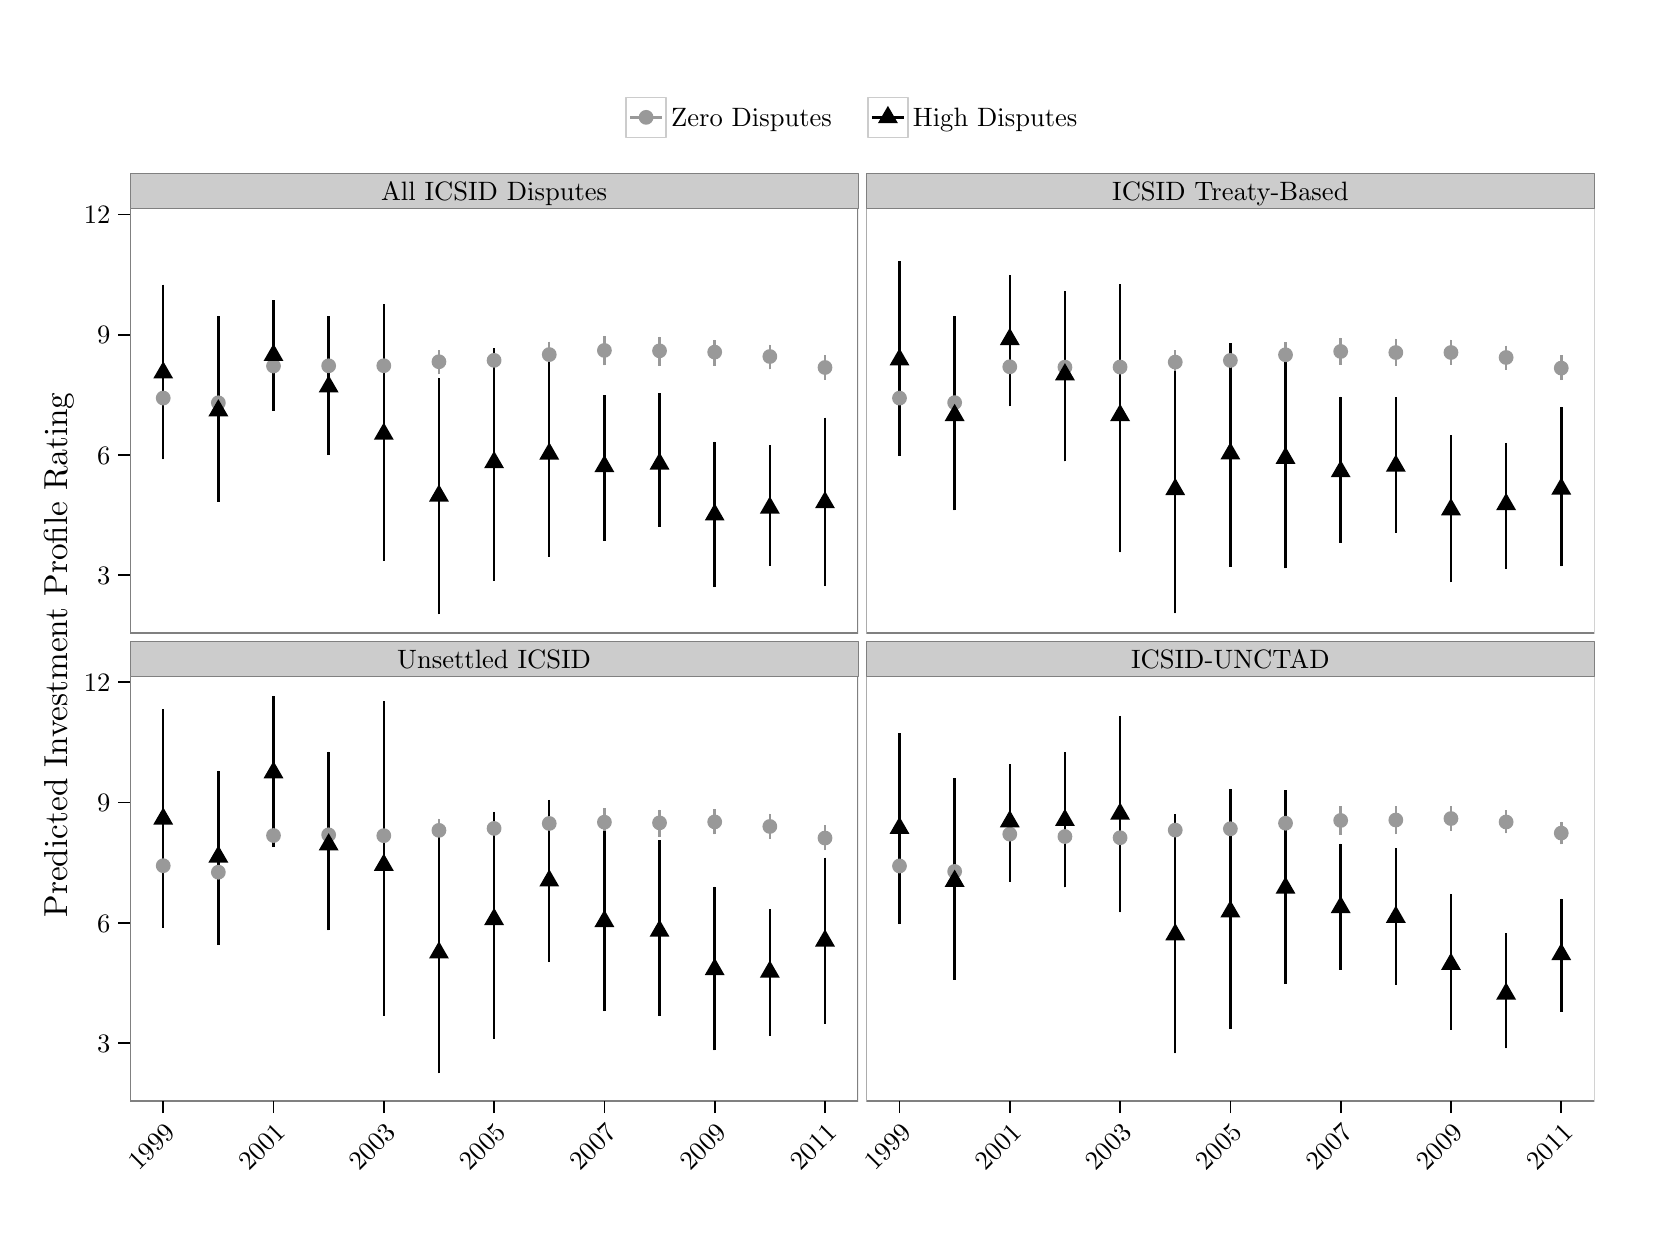
\begin{tikzpicture}[x=1pt,y=1pt]
\definecolor[named]{fillColor}{rgb}{1.00,1.00,1.00}
\path[use as bounding box,fill=fillColor,fill opacity=0.00] (0,0) rectangle (578.16,433.62);
\begin{scope}
\path[clip] (  0.00,  0.00) rectangle (578.16,433.62);
\definecolor[named]{drawColor}{rgb}{1.00,1.00,1.00}
\definecolor[named]{fillColor}{rgb}{1.00,1.00,1.00}

\path[draw=drawColor,line width= 0.6pt,line join=round,line cap=round,fill=fillColor] (  0.00,  0.00) rectangle (578.16,433.62);
\end{scope}
\begin{scope}
\path[clip] ( 37.02,214.77) rectangle (300.06,368.22);
\definecolor[named]{fillColor}{rgb}{1.00,1.00,1.00}

\path[fill=fillColor] ( 37.02,214.77) rectangle (300.06,368.22);
\definecolor[named]{drawColor}{rgb}{0.60,0.60,0.60}
\definecolor[named]{fillColor}{rgb}{0.60,0.60,0.60}

\path[draw=drawColor,line width= 0.9pt,line join=round,fill=fillColor] ( 48.98,293.67) -- ( 48.98,305.59);

\path[draw=drawColor,line width= 0.9pt,line join=round,fill=fillColor] ( 68.90,291.93) -- ( 68.90,304.29);

\path[draw=drawColor,line width= 0.9pt,line join=round,fill=fillColor] ( 88.83,307.70) -- ( 88.83,315.07);

\path[draw=drawColor,line width= 0.9pt,line join=round,fill=fillColor] (108.76,305.93) -- (108.76,317.28);

\path[draw=drawColor,line width= 0.9pt,line join=round,fill=fillColor] (128.69,306.46) -- (128.69,316.72);

\path[draw=drawColor,line width= 0.9pt,line join=round,fill=fillColor] (148.61,308.45) -- (148.61,317.07);

\path[draw=drawColor,line width= 0.9pt,line join=round,fill=fillColor] (168.54,309.24) -- (168.54,317.81);

\path[draw=drawColor,line width= 0.9pt,line join=round,fill=fillColor] (188.47,310.64) -- (188.47,320.16);

\path[draw=drawColor,line width= 0.9pt,line join=round,fill=fillColor] (208.40,311.61) -- (208.40,322.25);

\path[draw=drawColor,line width= 0.9pt,line join=round,fill=fillColor] (228.32,311.45) -- (228.32,321.98);

\path[draw=drawColor,line width= 0.9pt,line join=round,fill=fillColor] (248.25,311.52) -- (248.25,320.82);

\path[draw=drawColor,line width= 0.9pt,line join=round,fill=fillColor] (268.18,310.10) -- (268.18,319.07);

\path[draw=drawColor,line width= 0.9pt,line join=round,fill=fillColor] (288.11,306.38) -- (288.11,315.18);
\definecolor[named]{drawColor}{rgb}{0.00,0.00,0.00}
\definecolor[named]{fillColor}{rgb}{0.00,0.00,0.00}

\path[draw=drawColor,line width= 0.9pt,line join=round,fill=fillColor] ( 48.98,277.65) -- ( 48.98,340.81);

\path[draw=drawColor,line width= 0.9pt,line join=round,fill=fillColor] ( 68.90,262.34) -- ( 68.90,329.49);

\path[draw=drawColor,line width= 0.9pt,line join=round,fill=fillColor] ( 88.83,295.23) -- ( 88.83,335.12);

\path[draw=drawColor,line width= 0.9pt,line join=round,fill=fillColor] (108.76,279.19) -- (108.76,329.36);

\path[draw=drawColor,line width= 0.9pt,line join=round,fill=fillColor] (128.69,240.98) -- (128.69,333.61);

\path[draw=drawColor,line width= 0.9pt,line join=round,fill=fillColor] (148.61,221.74) -- (148.61,307.17);

\path[draw=drawColor,line width= 0.9pt,line join=round,fill=fillColor] (168.54,233.78) -- (168.54,317.86);

\path[draw=drawColor,line width= 0.9pt,line join=round,fill=fillColor] (188.47,242.46) -- (188.47,316.24);

\path[draw=drawColor,line width= 0.9pt,line join=round,fill=fillColor] (208.40,248.30) -- (208.40,300.81);

\path[draw=drawColor,line width= 0.9pt,line join=round,fill=fillColor] (228.32,253.28) -- (228.32,301.49);

\path[draw=drawColor,line width= 0.9pt,line join=round,fill=fillColor] (248.25,231.43) -- (248.25,284.04);

\path[draw=drawColor,line width= 0.9pt,line join=round,fill=fillColor] (268.18,239.20) -- (268.18,282.77);

\path[draw=drawColor,line width= 0.9pt,line join=round,fill=fillColor] (288.11,231.84) -- (288.11,292.68);
\definecolor[named]{fillColor}{rgb}{0.60,0.60,0.60}

\path[fill=fillColor] ( 48.98,299.78) circle (  2.67);
\definecolor[named]{fillColor}{rgb}{0.00,0.00,0.00}

\path[fill=fillColor] ( 48.98,313.08) --
	( 52.57,306.86) --
	( 45.38,306.86) --
	cycle;
\definecolor[named]{fillColor}{rgb}{0.60,0.60,0.60}

\path[fill=fillColor] ( 68.90,298.06) circle (  2.67);
\definecolor[named]{fillColor}{rgb}{0.00,0.00,0.00}

\path[fill=fillColor] ( 68.90,299.40) --
	( 72.50,293.18) --
	( 65.31,293.18) --
	cycle;
\definecolor[named]{fillColor}{rgb}{0.60,0.60,0.60}

\path[fill=fillColor] ( 88.83,311.37) circle (  2.67);
\definecolor[named]{fillColor}{rgb}{0.00,0.00,0.00}

\path[fill=fillColor] ( 88.83,319.41) --
	( 92.42,313.18) --
	( 85.24,313.18) --
	cycle;
\definecolor[named]{fillColor}{rgb}{0.60,0.60,0.60}

\path[fill=fillColor] (108.76,311.43) circle (  2.67);
\definecolor[named]{fillColor}{rgb}{0.00,0.00,0.00}

\path[fill=fillColor] (108.76,308.05) --
	(112.35,301.83) --
	(105.17,301.83) --
	cycle;
\definecolor[named]{fillColor}{rgb}{0.60,0.60,0.60}

\path[fill=fillColor] (128.69,311.46) circle (  2.67);
\definecolor[named]{fillColor}{rgb}{0.00,0.00,0.00}

\path[fill=fillColor] (128.69,290.94) --
	(132.28,284.72) --
	(125.09,284.72) --
	cycle;
\definecolor[named]{fillColor}{rgb}{0.60,0.60,0.60}

\path[fill=fillColor] (148.61,312.90) circle (  2.67);
\definecolor[named]{fillColor}{rgb}{0.00,0.00,0.00}

\path[fill=fillColor] (148.61,268.61) --
	(152.21,262.38) --
	(145.02,262.38) --
	cycle;
\definecolor[named]{fillColor}{rgb}{0.60,0.60,0.60}

\path[fill=fillColor] (168.54,313.40) circle (  2.67);
\definecolor[named]{fillColor}{rgb}{0.00,0.00,0.00}

\path[fill=fillColor] (168.54,280.68) --
	(172.13,274.46) --
	(164.95,274.46) --
	cycle;
\definecolor[named]{fillColor}{rgb}{0.60,0.60,0.60}

\path[fill=fillColor] (188.47,315.49) circle (  2.67);
\definecolor[named]{fillColor}{rgb}{0.00,0.00,0.00}

\path[fill=fillColor] (188.47,283.79) --
	(192.06,277.57) --
	(184.88,277.57) --
	cycle;
\definecolor[named]{fillColor}{rgb}{0.60,0.60,0.60}

\path[fill=fillColor] (208.40,316.99) circle (  2.67);
\definecolor[named]{fillColor}{rgb}{0.00,0.00,0.00}

\path[fill=fillColor] (208.40,279.25) --
	(211.99,273.03) --
	(204.80,273.03) --
	cycle;
\definecolor[named]{fillColor}{rgb}{0.60,0.60,0.60}

\path[fill=fillColor] (228.32,316.84) circle (  2.67);
\definecolor[named]{fillColor}{rgb}{0.00,0.00,0.00}

\path[fill=fillColor] (228.32,280.17) --
	(231.92,273.95) --
	(224.73,273.95) --
	cycle;
\definecolor[named]{fillColor}{rgb}{0.60,0.60,0.60}

\path[fill=fillColor] (248.25,316.38) circle (  2.67);
\definecolor[named]{fillColor}{rgb}{0.00,0.00,0.00}

\path[fill=fillColor] (248.25,261.76) --
	(251.84,255.54) --
	(244.66,255.54) --
	cycle;
\definecolor[named]{fillColor}{rgb}{0.60,0.60,0.60}

\path[fill=fillColor] (268.18,314.79) circle (  2.67);
\definecolor[named]{fillColor}{rgb}{0.00,0.00,0.00}

\path[fill=fillColor] (268.18,264.27) --
	(271.77,258.04) --
	(264.59,258.04) --
	cycle;
\definecolor[named]{fillColor}{rgb}{0.60,0.60,0.60}

\path[fill=fillColor] (288.11,310.83) circle (  2.67);
\definecolor[named]{fillColor}{rgb}{0.00,0.00,0.00}

\path[fill=fillColor] (288.11,266.20) --
	(291.70,259.97) --
	(284.51,259.97) --
	cycle;
\definecolor[named]{drawColor}{rgb}{0.50,0.50,0.50}

\path[draw=drawColor,line width= 0.6pt,line join=round,line cap=round] ( 37.02,214.77) rectangle (300.06,368.22);
\end{scope}
\begin{scope}
\path[clip] (303.07,214.77) rectangle (566.12,368.22);
\definecolor[named]{fillColor}{rgb}{1.00,1.00,1.00}

\path[fill=fillColor] (303.07,214.77) rectangle (566.12,368.22);
\definecolor[named]{drawColor}{rgb}{0.60,0.60,0.60}
\definecolor[named]{fillColor}{rgb}{0.60,0.60,0.60}

\path[draw=drawColor,line width= 0.9pt,line join=round,fill=fillColor] (315.03,293.78) -- (315.03,305.84);

\path[draw=drawColor,line width= 0.9pt,line join=round,fill=fillColor] (334.96,291.95) -- (334.96,304.13);

\path[draw=drawColor,line width= 0.9pt,line join=round,fill=fillColor] (354.88,307.16) -- (354.88,314.84);

\path[draw=drawColor,line width= 0.9pt,line join=round,fill=fillColor] (374.81,305.98) -- (374.81,316.10);

\path[draw=drawColor,line width= 0.9pt,line join=round,fill=fillColor] (394.74,305.73) -- (394.74,316.18);

\path[draw=drawColor,line width= 0.9pt,line join=round,fill=fillColor] (414.67,308.47) -- (414.67,316.99);

\path[draw=drawColor,line width= 0.9pt,line join=round,fill=fillColor] (434.59,309.08) -- (434.59,317.58);

\path[draw=drawColor,line width= 0.9pt,line join=round,fill=fillColor] (454.52,310.77) -- (454.52,319.96);

\path[draw=drawColor,line width= 0.9pt,line join=round,fill=fillColor] (474.45,311.76) -- (474.45,321.65);

\path[draw=drawColor,line width= 0.9pt,line join=round,fill=fillColor] (494.38,311.49) -- (494.38,321.25);

\path[draw=drawColor,line width= 0.9pt,line join=round,fill=fillColor] (514.30,311.80) -- (514.30,320.87);

\path[draw=drawColor,line width= 0.9pt,line join=round,fill=fillColor] (534.23,310.00) -- (534.23,318.75);

\path[draw=drawColor,line width= 0.9pt,line join=round,fill=fillColor] (554.16,306.27) -- (554.16,315.18);
\definecolor[named]{drawColor}{rgb}{0.00,0.00,0.00}
\definecolor[named]{fillColor}{rgb}{0.00,0.00,0.00}

\path[draw=drawColor,line width= 0.9pt,line join=round,fill=fillColor] (315.03,278.99) -- (315.03,349.30);

\path[draw=drawColor,line width= 0.9pt,line join=round,fill=fillColor] (334.96,259.18) -- (334.96,329.45);

\path[draw=drawColor,line width= 0.9pt,line join=round,fill=fillColor] (354.88,296.83) -- (354.88,344.32);

\path[draw=drawColor,line width= 0.9pt,line join=round,fill=fillColor] (374.81,276.90) -- (374.81,338.49);

\path[draw=drawColor,line width= 0.9pt,line join=round,fill=fillColor] (394.74,243.99) -- (394.74,340.82);

\path[draw=drawColor,line width= 0.9pt,line join=round,fill=fillColor] (414.67,221.97) -- (414.67,309.69);

\path[draw=drawColor,line width= 0.9pt,line join=round,fill=fillColor] (434.59,238.83) -- (434.59,319.61);

\path[draw=drawColor,line width= 0.9pt,line join=round,fill=fillColor] (454.52,238.22) -- (454.52,316.91);

\path[draw=drawColor,line width= 0.9pt,line join=round,fill=fillColor] (474.45,247.41) -- (474.45,300.28);

\path[draw=drawColor,line width= 0.9pt,line join=round,fill=fillColor] (494.38,251.06) -- (494.38,300.07);

\path[draw=drawColor,line width= 0.9pt,line join=round,fill=fillColor] (514.30,233.31) -- (514.30,286.29);

\path[draw=drawColor,line width= 0.9pt,line join=round,fill=fillColor] (534.23,238.00) -- (534.23,283.55);

\path[draw=drawColor,line width= 0.9pt,line join=round,fill=fillColor] (554.16,238.96) -- (554.16,296.55);
\definecolor[named]{fillColor}{rgb}{0.60,0.60,0.60}

\path[fill=fillColor] (315.03,299.76) circle (  2.67);
\definecolor[named]{fillColor}{rgb}{0.00,0.00,0.00}

\path[fill=fillColor] (315.03,317.80) --
	(318.62,311.58) --
	(311.44,311.58) --
	cycle;
\definecolor[named]{fillColor}{rgb}{0.60,0.60,0.60}

\path[fill=fillColor] (334.96,298.12) circle (  2.67);
\definecolor[named]{fillColor}{rgb}{0.00,0.00,0.00}

\path[fill=fillColor] (334.96,297.70) --
	(338.55,291.48) --
	(331.36,291.48) --
	cycle;
\definecolor[named]{fillColor}{rgb}{0.60,0.60,0.60}

\path[fill=fillColor] (354.88,311.08) circle (  2.67);
\definecolor[named]{fillColor}{rgb}{0.00,0.00,0.00}

\path[fill=fillColor] (354.88,325.15) --
	(358.48,318.92) --
	(351.29,318.92) --
	cycle;
\definecolor[named]{fillColor}{rgb}{0.60,0.60,0.60}

\path[fill=fillColor] (374.81,310.94) circle (  2.67);
\definecolor[named]{fillColor}{rgb}{0.00,0.00,0.00}

\path[fill=fillColor] (374.81,312.41) --
	(378.40,306.19) --
	(371.22,306.19) --
	cycle;
\definecolor[named]{fillColor}{rgb}{0.60,0.60,0.60}

\path[fill=fillColor] (394.74,310.98) circle (  2.67);
\definecolor[named]{fillColor}{rgb}{0.00,0.00,0.00}

\path[fill=fillColor] (394.74,297.69) --
	(398.33,291.47) --
	(391.15,291.47) --
	cycle;
\definecolor[named]{fillColor}{rgb}{0.60,0.60,0.60}

\path[fill=fillColor] (414.67,312.77) circle (  2.67);
\definecolor[named]{fillColor}{rgb}{0.00,0.00,0.00}

\path[fill=fillColor] (414.67,270.93) --
	(418.26,264.71) --
	(411.07,264.71) --
	cycle;
\definecolor[named]{fillColor}{rgb}{0.60,0.60,0.60}

\path[fill=fillColor] (434.59,313.37) circle (  2.67);
\definecolor[named]{fillColor}{rgb}{0.00,0.00,0.00}

\path[fill=fillColor] (434.59,283.82) --
	(438.19,277.59) --
	(431.00,277.59) --
	cycle;
\definecolor[named]{fillColor}{rgb}{0.60,0.60,0.60}

\path[fill=fillColor] (454.52,315.42) circle (  2.67);
\definecolor[named]{fillColor}{rgb}{0.00,0.00,0.00}

\path[fill=fillColor] (454.52,282.24) --
	(458.11,276.02) --
	(450.93,276.02) --
	cycle;
\definecolor[named]{fillColor}{rgb}{0.60,0.60,0.60}

\path[fill=fillColor] (474.45,316.62) circle (  2.67);
\definecolor[named]{fillColor}{rgb}{0.00,0.00,0.00}

\path[fill=fillColor] (474.45,277.40) --
	(478.04,271.18) --
	(470.86,271.18) --
	cycle;
\definecolor[named]{fillColor}{rgb}{0.60,0.60,0.60}

\path[fill=fillColor] (494.38,316.22) circle (  2.67);
\definecolor[named]{fillColor}{rgb}{0.00,0.00,0.00}

\path[fill=fillColor] (494.38,279.40) --
	(497.97,273.18) --
	(490.78,273.18) --
	cycle;
\definecolor[named]{fillColor}{rgb}{0.60,0.60,0.60}

\path[fill=fillColor] (514.30,316.24) circle (  2.67);
\definecolor[named]{fillColor}{rgb}{0.00,0.00,0.00}

\path[fill=fillColor] (514.30,263.64) --
	(517.90,257.42) --
	(510.71,257.42) --
	cycle;
\definecolor[named]{fillColor}{rgb}{0.60,0.60,0.60}

\path[fill=fillColor] (534.23,314.44) circle (  2.67);
\definecolor[named]{fillColor}{rgb}{0.00,0.00,0.00}

\path[fill=fillColor] (534.23,265.53) --
	(537.82,259.31) --
	(530.64,259.31) --
	cycle;
\definecolor[named]{fillColor}{rgb}{0.60,0.60,0.60}

\path[fill=fillColor] (554.16,310.60) circle (  2.67);
\definecolor[named]{fillColor}{rgb}{0.00,0.00,0.00}

\path[fill=fillColor] (554.16,271.14) --
	(557.75,264.92) --
	(550.57,264.92) --
	cycle;
\definecolor[named]{drawColor}{rgb}{0.50,0.50,0.50}

\path[draw=drawColor,line width= 0.6pt,line join=round,line cap=round] (303.07,214.77) rectangle (566.12,368.22);
\end{scope}
\begin{scope}
\path[clip] ( 37.02, 45.67) rectangle (300.06,199.12);
\definecolor[named]{fillColor}{rgb}{1.00,1.00,1.00}

\path[fill=fillColor] ( 37.02, 45.67) rectangle (300.06,199.12);
\definecolor[named]{drawColor}{rgb}{0.60,0.60,0.60}
\definecolor[named]{fillColor}{rgb}{0.60,0.60,0.60}

\path[draw=drawColor,line width= 0.9pt,line join=round,fill=fillColor] ( 48.98,125.38) -- ( 48.98,136.64);

\path[draw=drawColor,line width= 0.9pt,line join=round,fill=fillColor] ( 68.90,122.62) -- ( 68.90,134.68);

\path[draw=drawColor,line width= 0.9pt,line join=round,fill=fillColor] ( 88.83,137.99) -- ( 88.83,145.38);

\path[draw=drawColor,line width= 0.9pt,line join=round,fill=fillColor] (108.76,136.92) -- (108.76,146.80);

\path[draw=drawColor,line width= 0.9pt,line join=round,fill=fillColor] (128.69,136.43) -- (128.69,146.97);

\path[draw=drawColor,line width= 0.9pt,line join=round,fill=fillColor] (148.61,139.21) -- (148.61,147.84);

\path[draw=drawColor,line width= 0.9pt,line join=round,fill=fillColor] (168.54,139.98) -- (168.54,148.92);

\path[draw=drawColor,line width= 0.9pt,line join=round,fill=fillColor] (188.47,141.35) -- (188.47,150.56);

\path[draw=drawColor,line width= 0.9pt,line join=round,fill=fillColor] (208.40,141.52) -- (208.40,151.53);

\path[draw=drawColor,line width= 0.9pt,line join=round,fill=fillColor] (228.32,141.08) -- (228.32,151.10);

\path[draw=drawColor,line width= 0.9pt,line join=round,fill=fillColor] (248.25,142.10) -- (248.25,151.31);

\path[draw=drawColor,line width= 0.9pt,line join=round,fill=fillColor] (268.18,140.56) -- (268.18,149.61);

\path[draw=drawColor,line width= 0.9pt,line join=round,fill=fillColor] (288.11,136.44) -- (288.11,145.36);
\definecolor[named]{drawColor}{rgb}{0.00,0.00,0.00}
\definecolor[named]{fillColor}{rgb}{0.00,0.00,0.00}

\path[draw=drawColor,line width= 0.9pt,line join=round,fill=fillColor] ( 48.98,108.37) -- ( 48.98,187.25);

\path[draw=drawColor,line width= 0.9pt,line join=round,fill=fillColor] ( 68.90,102.13) -- ( 68.90,165.18);

\path[draw=drawColor,line width= 0.9pt,line join=round,fill=fillColor] ( 88.83,137.47) -- ( 88.83,192.15);

\path[draw=drawColor,line width= 0.9pt,line join=round,fill=fillColor] (108.76,107.39) -- (108.76,171.99);

\path[draw=drawColor,line width= 0.9pt,line join=round,fill=fillColor] (128.69, 76.50) -- (128.69,190.14);

\path[draw=drawColor,line width= 0.9pt,line join=round,fill=fillColor] (148.61, 55.81) -- (148.61,142.68);

\path[draw=drawColor,line width= 0.9pt,line join=round,fill=fillColor] (168.54, 68.20) -- (168.54,150.27);

\path[draw=drawColor,line width= 0.9pt,line join=round,fill=fillColor] (188.47, 95.95) -- (188.47,154.62);

\path[draw=drawColor,line width= 0.9pt,line join=round,fill=fillColor] (208.40, 78.21) -- (208.40,143.42);

\path[draw=drawColor,line width= 0.9pt,line join=round,fill=fillColor] (228.32, 76.53) -- (228.32,140.01);

\path[draw=drawColor,line width= 0.9pt,line join=round,fill=fillColor] (248.25, 64.08) -- (248.25,123.27);

\path[draw=drawColor,line width= 0.9pt,line join=round,fill=fillColor] (268.18, 69.38) -- (268.18,115.03);

\path[draw=drawColor,line width= 0.9pt,line join=round,fill=fillColor] (288.11, 73.63) -- (288.11,133.71);
\definecolor[named]{fillColor}{rgb}{0.60,0.60,0.60}

\path[fill=fillColor] ( 48.98,130.79) circle (  2.67);
\definecolor[named]{fillColor}{rgb}{0.00,0.00,0.00}

\path[fill=fillColor] ( 48.98,151.88) --
	( 52.57,145.66) --
	( 45.38,145.66) --
	cycle;
\definecolor[named]{fillColor}{rgb}{0.60,0.60,0.60}

\path[fill=fillColor] ( 68.90,128.45) circle (  2.67);
\definecolor[named]{fillColor}{rgb}{0.00,0.00,0.00}

\path[fill=fillColor] ( 68.90,138.16) --
	( 72.50,131.93) --
	( 65.31,131.93) --
	cycle;
\definecolor[named]{fillColor}{rgb}{0.60,0.60,0.60}

\path[fill=fillColor] ( 88.83,141.70) circle (  2.67);
\definecolor[named]{fillColor}{rgb}{0.00,0.00,0.00}

\path[fill=fillColor] ( 88.83,168.61) --
	( 92.42,162.39) --
	( 85.24,162.39) --
	cycle;
\definecolor[named]{fillColor}{rgb}{0.60,0.60,0.60}

\path[fill=fillColor] (108.76,141.95) circle (  2.67);
\definecolor[named]{fillColor}{rgb}{0.00,0.00,0.00}

\path[fill=fillColor] (108.76,142.56) --
	(112.35,136.34) --
	(105.17,136.34) --
	cycle;
\definecolor[named]{fillColor}{rgb}{0.60,0.60,0.60}

\path[fill=fillColor] (128.69,141.65) circle (  2.67);
\definecolor[named]{fillColor}{rgb}{0.00,0.00,0.00}

\path[fill=fillColor] (128.69,135.19) --
	(132.28,128.97) --
	(125.09,128.97) --
	cycle;
\definecolor[named]{fillColor}{rgb}{0.60,0.60,0.60}

\path[fill=fillColor] (148.61,143.57) circle (  2.67);
\definecolor[named]{fillColor}{rgb}{0.00,0.00,0.00}

\path[fill=fillColor] (148.61,103.50) --
	(152.21, 97.28) --
	(145.02, 97.28) --
	cycle;
\definecolor[named]{fillColor}{rgb}{0.60,0.60,0.60}

\path[fill=fillColor] (168.54,144.27) circle (  2.67);
\definecolor[named]{fillColor}{rgb}{0.00,0.00,0.00}

\path[fill=fillColor] (168.54,115.58) --
	(172.13,109.36) --
	(164.95,109.36) --
	cycle;
\definecolor[named]{fillColor}{rgb}{0.60,0.60,0.60}

\path[fill=fillColor] (188.47,146.06) circle (  2.67);
\definecolor[named]{fillColor}{rgb}{0.00,0.00,0.00}

\path[fill=fillColor] (188.47,129.51) --
	(192.06,123.29) --
	(184.88,123.29) --
	cycle;
\definecolor[named]{fillColor}{rgb}{0.60,0.60,0.60}

\path[fill=fillColor] (208.40,146.52) circle (  2.67);
\definecolor[named]{fillColor}{rgb}{0.00,0.00,0.00}

\path[fill=fillColor] (208.40,114.87) --
	(211.99,108.64) --
	(204.80,108.64) --
	cycle;
\definecolor[named]{fillColor}{rgb}{0.60,0.60,0.60}

\path[fill=fillColor] (228.32,146.28) circle (  2.67);
\definecolor[named]{fillColor}{rgb}{0.00,0.00,0.00}

\path[fill=fillColor] (228.32,111.36) --
	(231.92,105.14) --
	(224.73,105.14) --
	cycle;
\definecolor[named]{fillColor}{rgb}{0.60,0.60,0.60}

\path[fill=fillColor] (248.25,146.63) circle (  2.67);
\definecolor[named]{fillColor}{rgb}{0.00,0.00,0.00}

\path[fill=fillColor] (248.25, 97.50) --
	(251.84, 91.27) --
	(244.66, 91.27) --
	cycle;
\definecolor[named]{fillColor}{rgb}{0.60,0.60,0.60}

\path[fill=fillColor] (268.18,144.98) circle (  2.67);
\definecolor[named]{fillColor}{rgb}{0.00,0.00,0.00}

\path[fill=fillColor] (268.18, 96.58) --
	(271.77, 90.36) --
	(264.59, 90.36) --
	cycle;
\definecolor[named]{fillColor}{rgb}{0.60,0.60,0.60}

\path[fill=fillColor] (288.11,140.79) circle (  2.67);
\definecolor[named]{fillColor}{rgb}{0.00,0.00,0.00}

\path[fill=fillColor] (288.11,107.82) --
	(291.70,101.60) --
	(284.51,101.60) --
	cycle;
\definecolor[named]{drawColor}{rgb}{0.50,0.50,0.50}

\path[draw=drawColor,line width= 0.6pt,line join=round,line cap=round] ( 37.02, 45.67) rectangle (300.06,199.12);
\end{scope}
\begin{scope}
\path[clip] (303.07, 45.67) rectangle (566.12,199.12);
\definecolor[named]{fillColor}{rgb}{1.00,1.00,1.00}

\path[fill=fillColor] (303.07, 45.67) rectangle (566.12,199.12);
\definecolor[named]{drawColor}{rgb}{0.60,0.60,0.60}
\definecolor[named]{fillColor}{rgb}{0.60,0.60,0.60}

\path[draw=drawColor,line width= 0.9pt,line join=round,fill=fillColor] (315.03,124.77) -- (315.03,136.40);

\path[draw=drawColor,line width= 0.9pt,line join=round,fill=fillColor] (334.96,122.55) -- (334.96,134.49);

\path[draw=drawColor,line width= 0.9pt,line join=round,fill=fillColor] (354.88,138.58) -- (354.88,146.09);

\path[draw=drawColor,line width= 0.9pt,line join=round,fill=fillColor] (374.81,135.46) -- (374.81,146.59);

\path[draw=drawColor,line width= 0.9pt,line join=round,fill=fillColor] (394.74,135.88) -- (394.74,145.95);

\path[draw=drawColor,line width= 0.9pt,line join=round,fill=fillColor] (414.67,139.39) -- (414.67,147.97);

\path[draw=drawColor,line width= 0.9pt,line join=round,fill=fillColor] (434.59,139.78) -- (434.59,148.45);

\path[draw=drawColor,line width= 0.9pt,line join=round,fill=fillColor] (454.52,141.53) -- (454.52,150.88);

\path[draw=drawColor,line width= 0.9pt,line join=round,fill=fillColor] (474.45,141.91) -- (474.45,152.29);

\path[draw=drawColor,line width= 0.9pt,line join=round,fill=fillColor] (494.38,142.20) -- (494.38,152.36);

\path[draw=drawColor,line width= 0.9pt,line join=round,fill=fillColor] (514.30,143.35) -- (514.30,152.28);

\path[draw=drawColor,line width= 0.9pt,line join=round,fill=fillColor] (534.23,142.45) -- (534.23,150.85);

\path[draw=drawColor,line width= 0.9pt,line join=round,fill=fillColor] (554.16,138.48) -- (554.16,146.68);
\definecolor[named]{drawColor}{rgb}{0.00,0.00,0.00}
\definecolor[named]{fillColor}{rgb}{0.00,0.00,0.00}

\path[draw=drawColor,line width= 0.9pt,line join=round,fill=fillColor] (315.03,109.70) -- (315.03,178.73);

\path[draw=drawColor,line width= 0.9pt,line join=round,fill=fillColor] (334.96, 89.60) -- (334.96,162.56);

\path[draw=drawColor,line width= 0.9pt,line join=round,fill=fillColor] (354.88,124.91) -- (354.88,167.47);

\path[draw=drawColor,line width= 0.9pt,line join=round,fill=fillColor] (374.81,122.92) -- (374.81,171.79);

\path[draw=drawColor,line width= 0.9pt,line join=round,fill=fillColor] (394.74,113.96) -- (394.74,184.97);

\path[draw=drawColor,line width= 0.9pt,line join=round,fill=fillColor] (414.67, 62.98) -- (414.67,149.42);

\path[draw=drawColor,line width= 0.9pt,line join=round,fill=fillColor] (434.59, 71.72) -- (434.59,158.52);

\path[draw=drawColor,line width= 0.9pt,line join=round,fill=fillColor] (454.52, 88.23) -- (454.52,158.15);

\path[draw=drawColor,line width= 0.9pt,line join=round,fill=fillColor] (474.45, 93.25) -- (474.45,138.81);

\path[draw=drawColor,line width= 0.9pt,line join=round,fill=fillColor] (494.38, 87.78) -- (494.38,137.21);

\path[draw=drawColor,line width= 0.9pt,line join=round,fill=fillColor] (514.30, 71.48) -- (514.30,120.63);

\path[draw=drawColor,line width= 0.9pt,line join=round,fill=fillColor] (534.23, 64.78) -- (534.23,106.32);

\path[draw=drawColor,line width= 0.9pt,line join=round,fill=fillColor] (554.16, 77.99) -- (554.16,118.94);
\definecolor[named]{fillColor}{rgb}{0.60,0.60,0.60}

\path[fill=fillColor] (315.03,130.70) circle (  2.67);
\definecolor[named]{fillColor}{rgb}{0.00,0.00,0.00}

\path[fill=fillColor] (315.03,148.52) --
	(318.62,142.30) --
	(311.44,142.30) --
	cycle;
\definecolor[named]{fillColor}{rgb}{0.60,0.60,0.60}

\path[fill=fillColor] (334.96,128.73) circle (  2.67);
\definecolor[named]{fillColor}{rgb}{0.00,0.00,0.00}

\path[fill=fillColor] (334.96,129.39) --
	(338.55,123.16) --
	(331.36,123.16) --
	cycle;
\definecolor[named]{fillColor}{rgb}{0.60,0.60,0.60}

\path[fill=fillColor] (354.88,142.20) circle (  2.67);
\definecolor[named]{fillColor}{rgb}{0.00,0.00,0.00}

\path[fill=fillColor] (354.88,150.89) --
	(358.48,144.67) --
	(351.29,144.67) --
	cycle;
\definecolor[named]{fillColor}{rgb}{0.60,0.60,0.60}

\path[fill=fillColor] (374.81,141.34) circle (  2.67);
\definecolor[named]{fillColor}{rgb}{0.00,0.00,0.00}

\path[fill=fillColor] (374.81,151.38) --
	(378.40,145.16) --
	(371.22,145.16) --
	cycle;
\definecolor[named]{fillColor}{rgb}{0.60,0.60,0.60}

\path[fill=fillColor] (394.74,140.90) circle (  2.67);
\definecolor[named]{fillColor}{rgb}{0.00,0.00,0.00}

\path[fill=fillColor] (394.74,153.66) --
	(398.33,147.43) --
	(391.15,147.43) --
	cycle;
\definecolor[named]{fillColor}{rgb}{0.60,0.60,0.60}

\path[fill=fillColor] (414.67,143.66) circle (  2.67);
\definecolor[named]{fillColor}{rgb}{0.00,0.00,0.00}

\path[fill=fillColor] (414.67,110.05) --
	(418.26,103.83) --
	(411.07,103.83) --
	cycle;
\definecolor[named]{fillColor}{rgb}{0.60,0.60,0.60}

\path[fill=fillColor] (434.59,144.13) circle (  2.67);
\definecolor[named]{fillColor}{rgb}{0.00,0.00,0.00}

\path[fill=fillColor] (434.59,118.36) --
	(438.19,112.14) --
	(431.00,112.14) --
	cycle;
\definecolor[named]{fillColor}{rgb}{0.60,0.60,0.60}

\path[fill=fillColor] (454.52,146.15) circle (  2.67);
\definecolor[named]{fillColor}{rgb}{0.00,0.00,0.00}

\path[fill=fillColor] (454.52,126.92) --
	(458.11,120.70) --
	(450.93,120.70) --
	cycle;
\definecolor[named]{fillColor}{rgb}{0.60,0.60,0.60}

\path[fill=fillColor] (474.45,147.15) circle (  2.67);
\definecolor[named]{fillColor}{rgb}{0.00,0.00,0.00}

\path[fill=fillColor] (474.45,119.91) --
	(478.04,113.69) --
	(470.86,113.69) --
	cycle;
\definecolor[named]{fillColor}{rgb}{0.60,0.60,0.60}

\path[fill=fillColor] (494.38,147.30) circle (  2.67);
\definecolor[named]{fillColor}{rgb}{0.00,0.00,0.00}

\path[fill=fillColor] (494.38,116.40) --
	(497.97,110.17) --
	(490.78,110.17) --
	cycle;
\definecolor[named]{fillColor}{rgb}{0.60,0.60,0.60}

\path[fill=fillColor] (514.30,147.83) circle (  2.67);
\definecolor[named]{fillColor}{rgb}{0.00,0.00,0.00}

\path[fill=fillColor] (514.30, 99.36) --
	(517.90, 93.13) --
	(510.71, 93.13) --
	cycle;
\definecolor[named]{fillColor}{rgb}{0.60,0.60,0.60}

\path[fill=fillColor] (534.23,146.59) circle (  2.67);
\definecolor[named]{fillColor}{rgb}{0.00,0.00,0.00}

\path[fill=fillColor] (534.23, 88.64) --
	(537.82, 82.42) --
	(530.64, 82.42) --
	cycle;
\definecolor[named]{fillColor}{rgb}{0.60,0.60,0.60}

\path[fill=fillColor] (554.16,142.58) circle (  2.67);
\definecolor[named]{fillColor}{rgb}{0.00,0.00,0.00}

\path[fill=fillColor] (554.16,102.90) --
	(557.75, 96.68) --
	(550.57, 96.68) --
	cycle;
\definecolor[named]{drawColor}{rgb}{0.50,0.50,0.50}

\path[draw=drawColor,line width= 0.6pt,line join=round,line cap=round] (303.07, 45.67) rectangle (566.12,199.12);
\end{scope}
\begin{scope}
\path[clip] (  0.00,  0.00) rectangle (578.16,433.62);
\definecolor[named]{drawColor}{rgb}{0.50,0.50,0.50}
\definecolor[named]{fillColor}{rgb}{0.80,0.80,0.80}

\path[draw=drawColor,line width= 0.2pt,line join=round,line cap=round,fill=fillColor] ( 37.02,368.22) rectangle (300.06,380.85);
\definecolor[named]{drawColor}{rgb}{0.00,0.00,0.00}

\node[text=drawColor,anchor=base,inner sep=0pt, outer sep=0pt, scale=  0.96] at (168.54,371.23) {All ICSID Disputes};
\end{scope}
\begin{scope}
\path[clip] (  0.00,  0.00) rectangle (578.16,433.62);
\definecolor[named]{drawColor}{rgb}{0.50,0.50,0.50}
\definecolor[named]{fillColor}{rgb}{0.80,0.80,0.80}

\path[draw=drawColor,line width= 0.2pt,line join=round,line cap=round,fill=fillColor] (303.07,368.22) rectangle (566.12,380.85);
\definecolor[named]{drawColor}{rgb}{0.00,0.00,0.00}

\node[text=drawColor,anchor=base,inner sep=0pt, outer sep=0pt, scale=  0.96] at (434.59,371.23) {ICSID Treaty-Based};
\end{scope}
\begin{scope}
\path[clip] (  0.00,  0.00) rectangle (578.16,433.62);
\definecolor[named]{drawColor}{rgb}{0.50,0.50,0.50}
\definecolor[named]{fillColor}{rgb}{0.80,0.80,0.80}

\path[draw=drawColor,line width= 0.2pt,line join=round,line cap=round,fill=fillColor] ( 37.02,199.12) rectangle (300.06,211.75);
\definecolor[named]{drawColor}{rgb}{0.00,0.00,0.00}

\node[text=drawColor,anchor=base,inner sep=0pt, outer sep=0pt, scale=  0.96] at (168.54,202.13) {Unsettled ICSID};
\end{scope}
\begin{scope}
\path[clip] (  0.00,  0.00) rectangle (578.16,433.62);
\definecolor[named]{drawColor}{rgb}{0.50,0.50,0.50}
\definecolor[named]{fillColor}{rgb}{0.80,0.80,0.80}

\path[draw=drawColor,line width= 0.2pt,line join=round,line cap=round,fill=fillColor] (303.07,199.12) rectangle (566.12,211.75);
\definecolor[named]{drawColor}{rgb}{0.00,0.00,0.00}

\node[text=drawColor,anchor=base,inner sep=0pt, outer sep=0pt, scale=  0.96] at (434.59,202.13) {ICSID-UNCTAD};
\end{scope}
\begin{scope}
\path[clip] (  0.00,  0.00) rectangle (578.16,433.62);
\definecolor[named]{drawColor}{rgb}{0.00,0.00,0.00}

\node[text=drawColor,anchor=base east,inner sep=0pt, outer sep=0pt, scale=  0.96] at ( 29.91,232.42) {3};

\node[text=drawColor,anchor=base east,inner sep=0pt, outer sep=0pt, scale=  0.96] at ( 29.91,275.90) {6};

\node[text=drawColor,anchor=base east,inner sep=0pt, outer sep=0pt, scale=  0.96] at ( 29.91,319.38) {9};

\node[text=drawColor,anchor=base east,inner sep=0pt, outer sep=0pt, scale=  0.96] at ( 29.91,362.86) {12};
\end{scope}
\begin{scope}
\path[clip] (  0.00,  0.00) rectangle (578.16,433.62);
\definecolor[named]{drawColor}{rgb}{0.00,0.00,0.00}

\path[draw=drawColor,line width= 0.6pt,line join=round] ( 32.75,235.73) --
	( 37.02,235.73);

\path[draw=drawColor,line width= 0.6pt,line join=round] ( 32.75,279.21) --
	( 37.02,279.21);

\path[draw=drawColor,line width= 0.6pt,line join=round] ( 32.75,322.68) --
	( 37.02,322.68);

\path[draw=drawColor,line width= 0.6pt,line join=round] ( 32.75,366.16) --
	( 37.02,366.16);
\end{scope}
\begin{scope}
\path[clip] (  0.00,  0.00) rectangle (578.16,433.62);
\definecolor[named]{drawColor}{rgb}{0.00,0.00,0.00}

\node[text=drawColor,anchor=base east,inner sep=0pt, outer sep=0pt, scale=  0.96] at ( 29.91, 63.33) {3};

\node[text=drawColor,anchor=base east,inner sep=0pt, outer sep=0pt, scale=  0.96] at ( 29.91,106.81) {6};

\node[text=drawColor,anchor=base east,inner sep=0pt, outer sep=0pt, scale=  0.96] at ( 29.91,150.28) {9};

\node[text=drawColor,anchor=base east,inner sep=0pt, outer sep=0pt, scale=  0.96] at ( 29.91,193.76) {12};
\end{scope}
\begin{scope}
\path[clip] (  0.00,  0.00) rectangle (578.16,433.62);
\definecolor[named]{drawColor}{rgb}{0.00,0.00,0.00}

\path[draw=drawColor,line width= 0.6pt,line join=round] ( 32.75, 66.63) --
	( 37.02, 66.63);

\path[draw=drawColor,line width= 0.6pt,line join=round] ( 32.75,110.11) --
	( 37.02,110.11);

\path[draw=drawColor,line width= 0.6pt,line join=round] ( 32.75,153.59) --
	( 37.02,153.59);

\path[draw=drawColor,line width= 0.6pt,line join=round] ( 32.75,197.07) --
	( 37.02,197.07);
\end{scope}
\begin{scope}
\path[clip] (  0.00,  0.00) rectangle (578.16,433.62);
\definecolor[named]{drawColor}{rgb}{0.00,0.00,0.00}

\path[draw=drawColor,line width= 0.6pt,line join=round] ( 48.98, 41.40) --
	( 48.98, 45.67);

\path[draw=drawColor,line width= 0.6pt,line join=round] ( 88.83, 41.40) --
	( 88.83, 45.67);

\path[draw=drawColor,line width= 0.6pt,line join=round] (128.69, 41.40) --
	(128.69, 45.67);

\path[draw=drawColor,line width= 0.6pt,line join=round] (168.54, 41.40) --
	(168.54, 45.67);

\path[draw=drawColor,line width= 0.6pt,line join=round] (208.40, 41.40) --
	(208.40, 45.67);

\path[draw=drawColor,line width= 0.6pt,line join=round] (248.25, 41.40) --
	(248.25, 45.67);

\path[draw=drawColor,line width= 0.6pt,line join=round] (288.11, 41.40) --
	(288.11, 45.67);
\end{scope}
\begin{scope}
\path[clip] (  0.00,  0.00) rectangle (578.16,433.62);
\definecolor[named]{drawColor}{rgb}{0.00,0.00,0.00}

\node[text=drawColor,rotate= 45.00,anchor=base east,inner sep=0pt, outer sep=0pt, scale=  0.96] at ( 53.65, 33.88) {1999};

\node[text=drawColor,rotate= 45.00,anchor=base east,inner sep=0pt, outer sep=0pt, scale=  0.96] at ( 93.51, 33.88) {2001};

\node[text=drawColor,rotate= 45.00,anchor=base east,inner sep=0pt, outer sep=0pt, scale=  0.96] at (133.36, 33.88) {2003};

\node[text=drawColor,rotate= 45.00,anchor=base east,inner sep=0pt, outer sep=0pt, scale=  0.96] at (173.22, 33.88) {2005};

\node[text=drawColor,rotate= 45.00,anchor=base east,inner sep=0pt, outer sep=0pt, scale=  0.96] at (213.07, 33.88) {2007};

\node[text=drawColor,rotate= 45.00,anchor=base east,inner sep=0pt, outer sep=0pt, scale=  0.96] at (252.93, 33.88) {2009};

\node[text=drawColor,rotate= 45.00,anchor=base east,inner sep=0pt, outer sep=0pt, scale=  0.96] at (292.78, 33.88) {2011};
\end{scope}
\begin{scope}
\path[clip] (  0.00,  0.00) rectangle (578.16,433.62);
\definecolor[named]{drawColor}{rgb}{0.00,0.00,0.00}

\path[draw=drawColor,line width= 0.6pt,line join=round] (315.03, 41.40) --
	(315.03, 45.67);

\path[draw=drawColor,line width= 0.6pt,line join=round] (354.88, 41.40) --
	(354.88, 45.67);

\path[draw=drawColor,line width= 0.6pt,line join=round] (394.74, 41.40) --
	(394.74, 45.67);

\path[draw=drawColor,line width= 0.6pt,line join=round] (434.59, 41.40) --
	(434.59, 45.67);

\path[draw=drawColor,line width= 0.6pt,line join=round] (474.45, 41.40) --
	(474.45, 45.67);

\path[draw=drawColor,line width= 0.6pt,line join=round] (514.30, 41.40) --
	(514.30, 45.67);

\path[draw=drawColor,line width= 0.6pt,line join=round] (554.16, 41.40) --
	(554.16, 45.67);
\end{scope}
\begin{scope}
\path[clip] (  0.00,  0.00) rectangle (578.16,433.62);
\definecolor[named]{drawColor}{rgb}{0.00,0.00,0.00}

\node[text=drawColor,rotate= 45.00,anchor=base east,inner sep=0pt, outer sep=0pt, scale=  0.96] at (319.71, 33.88) {1999};

\node[text=drawColor,rotate= 45.00,anchor=base east,inner sep=0pt, outer sep=0pt, scale=  0.96] at (359.56, 33.88) {2001};

\node[text=drawColor,rotate= 45.00,anchor=base east,inner sep=0pt, outer sep=0pt, scale=  0.96] at (399.41, 33.88) {2003};

\node[text=drawColor,rotate= 45.00,anchor=base east,inner sep=0pt, outer sep=0pt, scale=  0.96] at (439.27, 33.88) {2005};

\node[text=drawColor,rotate= 45.00,anchor=base east,inner sep=0pt, outer sep=0pt, scale=  0.96] at (479.12, 33.88) {2007};

\node[text=drawColor,rotate= 45.00,anchor=base east,inner sep=0pt, outer sep=0pt, scale=  0.96] at (518.98, 33.88) {2009};

\node[text=drawColor,rotate= 45.00,anchor=base east,inner sep=0pt, outer sep=0pt, scale=  0.96] at (558.83, 33.88) {2011};
\end{scope}
\begin{scope}
\path[clip] (  0.00,  0.00) rectangle (578.16,433.62);
\definecolor[named]{drawColor}{rgb}{0.00,0.00,0.00}

\node[text=drawColor,rotate= 90.00,anchor=base,inner sep=0pt, outer sep=0pt, scale=  1.20] at ( 14.29,206.94) {Predicted Investment Profile Rating};
\end{scope}
\begin{scope}
\path[clip] (  0.00,  0.00) rectangle (578.16,433.62);
\definecolor[named]{fillColor}{rgb}{1.00,1.00,1.00}

\path[fill=fillColor] (208.36,389.72) rectangle (394.78,412.71);
\end{scope}
\begin{scope}
\path[clip] (  0.00,  0.00) rectangle (578.16,433.62);
\definecolor[named]{drawColor}{rgb}{0.80,0.80,0.80}
\definecolor[named]{fillColor}{rgb}{1.00,1.00,1.00}

\path[draw=drawColor,line width= 0.6pt,line join=round,line cap=round,fill=fillColor] (216.24,393.99) rectangle (230.69,408.44);
\end{scope}
\begin{scope}
\path[clip] (  0.00,  0.00) rectangle (578.16,433.62);
\definecolor[named]{drawColor}{rgb}{0.60,0.60,0.60}

\path[draw=drawColor,line width= 0.9pt,line join=round] (217.68,401.21) -- (229.25,401.21);
\end{scope}
\begin{scope}
\path[clip] (  0.00,  0.00) rectangle (578.16,433.62);
\definecolor[named]{fillColor}{rgb}{0.60,0.60,0.60}

\path[fill=fillColor] (223.47,401.21) circle (  2.67);
\end{scope}
\begin{scope}
\path[clip] (  0.00,  0.00) rectangle (578.16,433.62);
\definecolor[named]{drawColor}{rgb}{0.80,0.80,0.80}
\definecolor[named]{fillColor}{rgb}{1.00,1.00,1.00}

\path[draw=drawColor,line width= 0.6pt,line join=round,line cap=round,fill=fillColor] (303.62,393.99) rectangle (318.08,408.44);
\end{scope}
\begin{scope}
\path[clip] (  0.00,  0.00) rectangle (578.16,433.62);
\definecolor[named]{drawColor}{rgb}{0.00,0.00,0.00}

\path[draw=drawColor,line width= 0.9pt,line join=round] (305.07,401.21) -- (316.63,401.21);
\end{scope}
\begin{scope}
\path[clip] (  0.00,  0.00) rectangle (578.16,433.62);
\definecolor[named]{fillColor}{rgb}{0.00,0.00,0.00}

\path[fill=fillColor] (310.85,405.36) --
	(314.44,399.14) --
	(307.26,399.14) --
	cycle;
\end{scope}
\begin{scope}
\path[clip] (  0.00,  0.00) rectangle (578.16,433.62);
\definecolor[named]{drawColor}{rgb}{0.00,0.00,0.00}

\node[text=drawColor,anchor=base west,inner sep=0pt, outer sep=0pt, scale=  0.96] at (232.50,397.91) {Zero Disputes $\; \; \;$};
\end{scope}
\begin{scope}
\path[clip] (  0.00,  0.00) rectangle (578.16,433.62);
\definecolor[named]{drawColor}{rgb}{0.00,0.00,0.00}

\node[text=drawColor,anchor=base west,inner sep=0pt, outer sep=0pt, scale=  0.96] at (319.89,397.91) {High Disputes $\; \; \;$};
\end{scope}
\end{tikzpicture}
}	
\end{figure}

\end{frame}
%%%%%%%%%%%%%%%%%%%%%%%%%%%%%%%%%%%%%%%%%

%%%%%%%%%%%%%%%%%%%%%%%%%%%%%%%%%%%%%%%%%
\begin{frame}
\frametitle{Newspaper Mentions of ICSID}

\begin{figure}[ht]
	\centering
	\resizebox{1\textwidth}{!}{\input{histICSID}}
\end{figure}

\end{frame}
%%%%%%%%%%%%%%%%%%%%%%%%%%%%%%%%%%%%%%%%%

% %%%%%%%%%%%%%%%%%%%%%%%%%%%%%%%%%%%%%%%%%
% % Maps
% \begin{frame}
% \frametitle{Geographic Spread of 2012 Probability Distribution}

% \begin{figure}
% 	\centering
% 	\vspace{-7mm}
% 	\begin{tabular}{ll}
%     \hspace{-7mm}	
%     \subfloat[][Polity$\geq$7]{
% 		\includegraphics[width=0.5\textwidth]{polGe7_2012_map}
%         \label{fig:map7}} &
%     \subfloat[][Polity$\geq$8]{
% 		\includegraphics[width=0.5\textwidth]{polGe8_2012_map}
%         \label{fig:map8}} \\
% 	\hspace{-7mm}	
%     \subfloat[][Polity$\geq$9]{
% 		\includegraphics[width=0.5\textwidth]{polGe9_2012_map}
%         \label{fig:map9}} &
%     \subfloat[][Polity$=$10]{
% 		\includegraphics[width=0.5\textwidth]{polGe10_2012_map}
%         \label{fig:map10}}
%     \end{tabular}
% \end{figure}

% \end{frame}
% %%%%%%%%%%%%%%%%%%%%%%%%%%%%%%%%%%%%%%%%%

% \section{SVM Performance}

% %%%%%%%%%%%%%%%%%%%%%%%%%%%%%%%%%%%%%%%%%
% \begin{frame}
% \frametitle{Out-of-Sample Aggregate Performance}

% \begin{figure}[ht]
% 	\centering
% 	\resizebox{1\textwidth}{!}{\input{aggStats.tex}}	
% \end{figure}

% \end{frame}
% %%%%%%%%%%%%%%%%%%%%%%%%%%%%%%%%%%%%%%%%%

% %%%%%%%%%%%%%%%%%%%%%%%%%%%%%%%%%%%%%%%%%
% % Separation plots
% \begin{frame}
% \frametitle{Out-of-Sample Separation Plots}

% \begin{figure}
% 	\centering
% 	\begin{tabular}{ll}
%     \hspace{-7mm}	
%     \subfloat[][Polity$\geq$7]{
% 		\resizebox{0.5\textwidth}{!}{\input{polGe7_sep.tex}}	
%         \label{fig:sep7}} &
%     \subfloat[][Polity$\geq$8]{
% 		\resizebox{0.5\textwidth}{!}{\input{polGe8_sep.tex}}	
%         \label{fig:sep8}} \\
% 	\hspace{-7mm}	
%     \subfloat[][Polity$\geq$9]{
% 		\resizebox{0.5\textwidth}{!}{\input{polGe9_sep.tex}}	
%         \label{fig:sep9}} &
%     \subfloat[][Polity$=$10]{
% 		\resizebox{0.5\textwidth}{!}{\input{polGe10_sep.tex}}	
%         \label{fig:sep10}}
%     \end{tabular}
% \end{figure}

% \end{frame}
% %%%%%%%%%%%%%%%%%%%%%%%%%%%%%%%%%%%%%%%%%

\end{document}